\documentclass[sigconf]{acmart}
\usepackage{subfig}
\usepackage{tabulary}
\usepackage{threeparttable}
\usepackage{hyperref}
\usepackage{relsize,xspace}
\usepackage[framemethod=tikz,
innerleftmargin=1pt,
innerrightmargin=1pt,
innertopmargin=1pt,
innerbottommargin=1pt,
skipabove=6pt,
skipbelow=6pt,
splittopskip=2pt,
splitbottomskip=2pt,
roundcorner = 0pt
]{mdframed}
\usepackage{listings}
\usepackage{multirow}
\usepackage{microtype}

\definecolor{light-gray-fork}{gray}{0.925}
\definecolor{light-gray-mainline}{gray}{0.8}
\definecolor{javared}{rgb}{0.6,0,0} % for strings
\definecolor{javagreen}{rgb}{0.25,0.5,0.35} % comments
\definecolor{javapurple}{rgb}{0.5,0,0.35} % keywords
\definecolor{javadocblue}{rgb}{0.25,0.35,0.75} % javadoc
\lstdefinestyle{all}{
	basicstyle=\fontsize{11}{11}\selectfont\ttfamily\footnotesize,
	numbers=none,
	xleftmargin=0.1cm,
	xrightmargin=0.1cm,
	stepnumber=1,
	showstringspaces=false,
	tabsize=1,
	breaklines=true,
	breakatwhitespace=false,
	frame=single,
	commentstyle=\color{gray}
}

\lstdefinestyle{result} {
	frame=none,
	escapechar=`,
	language=Java,
	basicstyle=\fontsize{11}{12}\scriptsize,
	postbreak=\mbox{\textcolor{gray}{$\hookrightarrow$}\space},
	keywordstyle=\color{javapurple}\bfseries,
	stringstyle=\color{javared},
	commentstyle=\color{javagreen},
	morecomment=[s][\color{javadocblue}]{/**}{*/},
	moredelim=**[is][\color{red}]{@@}{@@},
}

\lstdefinestyle{dataset} {
	frame=single,
	escapechar=`,
	language=Java,
	basicstyle=\fontsize{11}{12}\scriptsize,
	postbreak=\mbox{\textcolor{gray}{$\hookrightarrow$}\space},
	keywordstyle=\color{javapurple}\bfseries,
	stringstyle=\color{javared},
	commentstyle=\color{javagreen},
	morecomment=[s][\color{javadocblue}]{/**}{*/},
	moredelim=**[is][\color{red}]{@@}{@@},
}
\usepackage{array}
\newcommand*\rotbf[1]{\rotatebox{90}{\textbf{#1}}}
\newcommand{\specialcell}[2][c]{\begin{tabular}[#1]{@{}l@{}}#2\end{tabular}}
\newcommand{\specialcellbold}[2][c]{%
	\bfseries
	\begin{tabular}[#1]{@{}l@{}}#2\end{tabular}%
}
\newcommand\parhead[1]{\vspace{.26mm}\noindent\textbf{{#1}}.}  
\newcommand{\secref}[1]{Section~\ref{#1}}
\newcommand{\figref}[1]{Fig.~\ref{#1}}
\newcommand{\Figref}[1]{Figure~\ref{#1}}
\newcommand{\tabref}[1]{Table~\ref{#1}}
\newcommand{\lstref}[1]{Listing~\ref{#1}}

\newcommand{\mtnote}[1]{\textsuperscript{\TPTtagStyle{#1}}}
\newcommand\theader[1]{\textsf{{#1}}}
\newcommand\featureName[1]{\textit{\textsf{{#1}}}}
\newcommand\mformula[1]{$\mathnormal{{#1}}$}

\newcommand{\tb}[1]{{\textsf{TB}[\smaller\sffamily\color{blue} #1}]}
\newcommand{\rh}[1]{{\textsf{RH}[\smaller\sffamily\color{orange} #1}]}
\newcommand{\mm}[1]{{\textsf{MM}[\smaller\sffamily\color{green!10!orange!90!} #1}]}
\newcommand{\wm}[1]{{\textsf{WM}[\smaller\sffamily\color{red} #1}]}
\newcommand{\es}{ElasticSearch\xspace}

\usepackage{xcolor}

\newcommand{\quotebox}[3]{\vspace{.5em}\noindent\begin{tikzpicture}
\node[align=center,draw,thin,minimum width=\columnwidth,inner sep=2.2mm] (titlebox)%
{\parbox{0.95\columnwidth}{\noindent\textit{#2}}};\node[fill=white] (W) at ([xshift=#3]titlebox.south) {\small #1};%
\end{tikzpicture}}

\newcounter{recommendationno}
\newcommand{\recommendation}[1]{\refstepcounter{recommendationno}Recommendation \the\numexpr\value{recommendationno}~(\factor{#1})}
\newcounter{observationno}
\newcommand{\observation}[1]{\refstepcounter{observationno}Observation \the\numexpr\value{observationno}~(#1)}


\setcopyright{acmcopyright}
\copyrightyear{2020}
\acmYear{2020}
\acmDOI{}

\setcopyright{none}

\begin{document}
\title{Feature Defect Prediction}
\renewcommand{\shorttitle}{}

\author{Stefan Strüder}
\affiliation{University of Koblenz-Landau, Germany}

\author{Daniel Strüber}
\affiliation{Radboud University Nijmegen, Netherlands}

\author{Thorsten Berger}
\affiliation{Chalmers $|$ University of Gothenburg, Sweden}

\author{Mukelabai Mukelabai}
\affiliation{Chalmers $|$ University of Gothenburg, Sweden}

\renewcommand{\shortauthors}{}


\begin{abstract}
Software errors are a major nuisance in software development and can lead not only to damage to reputation but also to considerable financial losses for companies. For this reason, numerous techniques for detecting and predicting defects have been developed over the past decade, which are largely based on machine learning methods. These techniques are usually aimed at predicting defects at the file level. However, in recent years the popularity of feature-based software development has been increasing: a paradigm that relies on functional increments of a software system (features) and thus ensures a wide variability of the software product. A common implementation technique for features is based on annotations with preprocessor instructions, such as \texttt{\#IFDEF} and \texttt{\#IFNDEF}, whose code is spread over several files of the software source code ("code scattering"). A bug in such feature code can have far-reaching consequences for the functionality of the entire software. If a part of the feature code contains defects, the entire function of the feature becomes faulty and may lead to the failure of the entire functionality of the software (features are "cross-cutting"). This problem is the subject of this thesis. A prediction technique for defective features is developed, which is based on machine learning methods. The evaluation of eight classifiers, each based on an individual classification algorithm, shows that the feature-based dataset created for this thesis allows an accuracy of up to 84\% for the prediction of defective or defect-free features. It is also shown how the feature oriented aspect was integrated into the creation of the dataset and what results were achieved compared to the traditional file-based methodology. This comparison showed that the additional inclusion of the feature aspect in the file-based defect prediction does not have a significant impact on the prediction results.

\end{abstract}

\keywords{}

\maketitle

% !TEX root = ../thesis.tex

\chapter{Einleitung und Motivation}
\label{introduction}

Softwarefehler stellen einen erheblichen Auslöser für finanzielle Schäden und Rufschädigungen von Unternehmen dar. Solche Fehler reichen von kleineren \glqq Bugs\grqq{} bis hin zu schwerwiegenden Sicherheitslücken. Aus diesem Grund herrscht ein großes Interesse daran, einen Entwickler zu warnen, wenn er aktualisierten Softwarecode veröffentlicht, der möglicherweise einen oder mehrere Fehler beinhaltet. 

Zu diesem Zweck haben Forscher und Softwareentwickler im vergangenen Jahrzehnt verschiedene Techniken zur Fehlervorhersage entwickelt, die zu einem Großteil auf Methoden und Techniken des Machine Learnings basieren \cite{Challagulla2008}. Diese verwenden in der Regel historische Daten von fehlerhaften und fehlerfreien Änderungen an Softwaresystemen in Kombination mit einer sorgfältig zusammengestellten Menge von Attributen (in der Regel Features genannt\footnote{Um einem missverständlichen und doppeldeutigen Gebrauch des Feature-Begriffes vorzubeugen, wird für die hier verwendete Beschreibung der Charakteristika von Daten auch im weiteren Verlauf dieser Ausarbeitung der Begriff \glqq Attribute\grqq{} verwendet.}), um einen gegebenen Klassifikator zu trainieren \cite{Alsaeedi2019,Hammouri2018}. Dieser kann dann anschließend verwendet werden, um eine akkurate Vorhersage zu erhalten, ob eine neu erfolgte Änderung an einer Software fehlerhaft oder frei von Fehlern ist.

Die Auswahl an Algorithmen für die Klassifikation ist groß. Studien zeigen, dass aus dem Pool von verfügbaren Algorithmen sowohl Entscheidungsbaum-basierte (zum Beispiel J48, CART oder Random Forest) als auch Bayessche Algorithmen (zum Beispiel Na\"{\i}ve Bayes (NB), Bernoulli-NB oder multinomieller NB) die meistgenutzten sind \cite{Son2019}. Alternative Algorithmen sind beispielsweise Regression, k-Nearest-Neighbors oder künstliche neuronale Netze \cite{Challagulla2008}. Anzumerken ist allerdings, dass es keinen Konsens über den besten verfügbaren Algorithmus gibt, da jeder Algorithmus unterschiedliche Stärken und Schwächen für bestimmte Anwendungsfälle aufweist.

Das Ziel dieser Arbeit ist die Entwicklung einer solchen Vorhersagetechnik für Softwarefehler basierend auf Software-Features. Diese Features beschreiben Inkremente der Funktionalität eines Softwaresystems. Die auf diese Weise entwickelten Softwaresysteme heißen Software-Produktlinien und bestehen aus einer Menge von ähnlichen Softwareprodukten. Sie zeichnen sich dadurch aus, dass sie eine gemeinsame Menge von Features sowie eine gemeinsame Codebasis besitzen \cite{Thuem2014}. Durch das Vorhandensein verschiedener Features entlang der Softwareprodukte, kann eine breite Variabilität innerhalb einer Produktlinie erreicht werden. Eine detaillierte Einführung in den Themenkomplex von Software-Produktlinien und featurebasierter Softwareentwicklung kann in \hyperref[feat-develop]{Abschnitt 2.1} gefunden werden. Bei der Entwicklung der Vorhersagetechnik wird die Implementation von Features mittels Präprozessor-Anweisungen, wie \texttt{\#IFDEF} und \texttt{\#IFNDEF} (auch Präprozessor-Direktiven genannt) betrachtet. Dieser bisher in wissenschaftlichen Arbeiten nur einmal im Rahmen einer Fallstudie betrachtete Ansatz \cite{Queiroz2016} ist aufgrund mehrerer Gründe chancenreich:

\begin{enumerate}
\setlength{\itemsep}{-2pt}
\item Wenn ein bestimmtes Feature in der Vergangenheit mehr oder weniger fehleranfällig war, so ist eine Änderung, die das Feature aktualisiert, wahrscheinlich ebenfalls mehr oder weniger fehleranfällig. 
\item Features, die mehr oder weniger fehleranfällig scheinen, könnten besondere Eigenschaften haben, die im Rahmen der Fehlervorhersage verwendet werden können.
\item Code, der viel featuresspezifischen Code enthält (insbesondere die sogenannten Feature-Interaktionen), ist möglicherweise fehleranfälliger als sonstiger Code.
\end{enumerate}

Ein initiales und einfaches Beispiel für einen Softwarefehler innerhalb eines Features ist in \autoref{bug-code} dargestellt. Es ist zu erkennen, dass innerhalb des Codes des Features \texttt{print\_time} die \texttt{printf}-Anweisung einen Schreibfehler enthält, der dazu führt, dass der Featurecode nicht ausgeführt werden kann. Ferner kann fehlerhafter Featurecode dazu führen, dass die gesamte Funktionalität des Features und gegebenenfalls der gesamten Software beeinträchtigt oder verhindert wird. Ein reales Beispiel für einen Fehler aus dem Sourcecode des Softwareprojekts Vim ist in \autoref{fig:bug-example} dargestellt.

\begin{lstlisting}[language=Python, caption=Exemplarische Darstellung eines fehlerhaften Features, frame=single, label=bug-code]
int test() {
	  #IFDEF print_time
	  prntf("Current time: %s", time(&now));
	  #ENDIF

	  printf("Hello World!");
	  return 0;
  }
\end{lstlisting}
 
Das zuvor genannte Ziel der Arbeit setzt sich aus mehreren Teilzielen zusammen. Dazu zählen die Erstellung eines Datensets unter Einbezug des Feature-Aspekts (\hyperref[dataset-creation]{Kapitel 3}). Dieses Datenset dient wiederum zum Training einer repräsentativen Auswahl an Klassifikatoren (\hyperref[training]{Kapitel 4}) mit anschließender vergleichender Evaluation (\hyperref[evaluation]{Kapitel 5}) dieser. Zusätzlich wird das featurebasierte Datenset mit einem klassischen dateibasierten Datenset (\hyperref[classic-eval]{Abschnitt 5.2}) verglichen, dessen Entwicklung aus einer wissenschaftlichen Arbeit entnommen wurde \cite{Moser2008}. Ein genauer Überblick über die Forschungsziele befindet sich im nächsten Abschnitt.

Sollte sich im Rahmen der Evaluation einer dieser Klassifikatoren als besonders effektiv erweisen, so würde diese Arbeit den Stand der Technik hinsichtlich der Fehlervorhersage in Features vorantreiben und Organisationen erlauben, bessere Einblicke in die Fehleranfälligkeit von Änderungen in ihrer durch Variabilität geprägten Codebasis zu erhalten.

\section{Forschungsziele und Forschungsfragen}

Wie bereits in der Einleitung beschrieben, ist das übergeordnete Ziel dieser Arbeit die Entwicklung einer Vorhersagetechnik für Fehler in featurebasierter Software unter Zuhilfenahme von Methoden des Machine Learnings. Dazu ist vorgesehen, das Augenmerk hinsichtlich der Datengrundlage auf Commits des Versionierungssystems Git zu richten. Ein Commit beschreibt dabei die Freischaltung von Veränderungen an einer oder mehreren Dateien. Als Datenbasis für das Trainieren der Klassifikatoren dienen dann Commits, für die auf Grundlage eines automatisierten Verfahrens aus der Literatur eine Klassifikation in \glqq defekt\grqq{} und \glqq fehlerfrei\grqq{} verfügbar ist. Dies ermöglicht es, für ausstehende oder zukünftige Softwareversionen akkurate Vorhersagen zu treffen, ob diese Fehler beinhalten. So kann das Risiko der Konsequenzen von Softwarefehlern gesenkt werden.

Der Prozess der Entwicklung der Vorhersagetechnik ist in drei zu erreichende Forschungsziele eingeteilt. Jedem Forschungsziel werden Forschungsfragen zugeordnet, deren Aufklärung einen zusätzlichen Teil zur Erfüllung der Ziele beiträgt. Im Folgenden werden die Forschungsziele (RO – \glqq research objective\grqq) mit ihren zugehörigen Forschungsfragen (RQ – \glqq research question\grqq) vorgestellt. Die Beantwortung der Forschungsfragen erfolgt im weiteren Verlauf der Arbeit. Erkennbar sind die Antworten auf die Fragen an ihrer Einrahmung.

\label{research_objectives}

\fbox{\parbox{\linewidth}{RO1: Erstellung eines Datensets zum Trainieren von relevanten Machine-Learning-Klassifikatoren
\begin{itemize}
 \renewcommand{\labelitemi}{$\Rightarrow$}
 \setlength{\itemsep}{-2pt}
 \item RQ1a: Welche Daten kommen für die Erstellung des Datensets in Frage?
 \item RQ1b: Wie weit müssen die Daten vorverarbeitet werden, um sie für das Training nutzbar zu machen?
\end{itemize}}}

\fbox{\parbox{\linewidth}{RO2: Identifikation und Training einer Auswahl von relevanten Machine-Learning-Klassifikatoren basierend auf dem Datenset
\begin{itemize}
 \renewcommand{\labelitemi}{$\Rightarrow$}
 \setlength{\itemsep}{-2pt}
 \item RQ2: Welche Machine-Learning-Klassifikatoren kommen für die gegebene Aufgabe in Frage?
\end{itemize}}}

\fbox{\parbox{\linewidth}{RO3: Evaluation und Gegenüberstellung der Klassifikatoren sowie Vergleich zu einer klassischen Vorhersagetechnik, die keine Features nutzt
\begin{itemize}
 \renewcommand{\labelitemi}{$\Rightarrow$}
 \setlength{\itemsep}{-2pt}
 \item RQ3a: Welches Vorgehen bietet sich zum internen Vergleich der Klassifikatoren an?
 \item RQ3b: Welche Ergebnisse können bei der Vorhersage von fehlerhaften oder fehlerfreien Features erzielt werden?
 \item RQ3c: Wie lassen sich die Klassifikatoren mit einer klassischen Vorhersagetechnik, die keine Features nutzt, vergleichen?
 \item RQ3d: Wie beeinflusst die Verwendung von featurebasierten Metriken die dateibasierte Fehlervorhersage?
\end{itemize}}}

\label{phases_definition}

Zusätzlich zu den drei genannten Forschungszielen umfasst die Bearbeitung der Masterarbeit eine Vor- und Nachbereitung, sodass sich insgesamt fünf Arbeitsphasen ergeben:

\begin{itemize}
\setlength{\itemsep}{-2pt}
\item Vorbereitung
\item Abschluss des ersten Forschungsziels (\textit{Erstellung des Datensets})
\item Abschluss des zweiten Forschungsziels (\textit{Training von Machine-Learning-Klassifikatoren})
\item Abschluss des dritten Forschungsziels (\textit{Evaluation und Vergleich})
\item Nachbereitung
\end{itemize}

Diese Arbeitsphasen werden im kommenden Abschnitt anhand des verwendeten Forschungsdesigns näher erläutert.
%Als finale Vorhersagetechnik wird jener Klassifikator verwendet, der sich im Rahmen der Gegenüberstellung im Verlauf der Evaluation als am \glqq effektivsten\grqq{} erweist. Die Kriterien für die Beurteilung der Effektivität eines Klassifikators werden im Kapitel \glqq \hyperref[evaluation]{Evaluation}\grqq{} erläutert.

\section{Forschungsdesign}

Die für diese Arbeit gewählte Methodik basiert auf dem Prozessmodell \glqq Cross-Industry Standard Process for Data Mining\grqq, kurz CRISP-DM, nach Chapman et al. \cite{Chapman2000}. Es wird als Vorlage für die Arbeitsphasen zur Erreichung der Forschungsziele dieser Arbeit verwendet. Da sich der überwiegende praktische Teil dieser Arbeit auf Programmierung im Bereich des Machine Learning konzentriert, bildet das CRISP-DM Prozessmodell ein passendes vordefiniertes Vorgehen. Eine grafische Aufarbeitung des Prozessmodells mit seinen sechs zugehörigen Phasen sowie den Verbindungen zwischen ihnen ist in \autoref{fig:crisp1} dargestellt. 

\begin{figure}[ht]
    \centering
    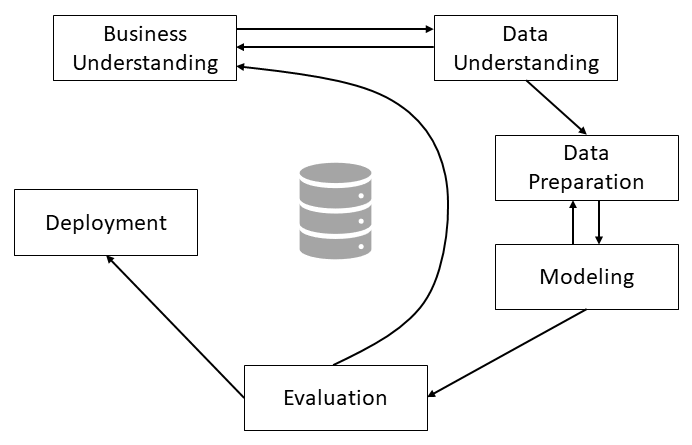
\includegraphics[width=0.6\textwidth]{images/CRISP-DM1}
    \caption{CRISP-DM Prozessmodell nach \cite{Chapman2000}}\label{fig:crisp1}
\end{figure}

Das CRISP-DM-Prozessmodell wurde, wie der ausgeschriebene Name bereits andeutet, ursprünglich für die Erarbeitung von Data-Mining-Projekten entwickelt, eignet sich jedoch auch zur Verwendung im Rahmen eines Machine Learning Projektes, da sich die in beiden Bereichen verwendeten Methoden und Prozesse zu einem erheblichen Teil überlagern. Ein Überblick über die sechs Phasen des Prozessmodells ist in \autoref{fig:crisp} dargestellt. Zusätzlich umfasst diese Abbildung die Zuordnung der Arbeitsphasen, die im \hyperref[phases_definition]{vorherigen Abschnitt} definiert wurden. Eine Erläuterung der Phasen des Prozessmodells erfolgt im Anschluss. 

\begin{figure}[ht]
    \centering
    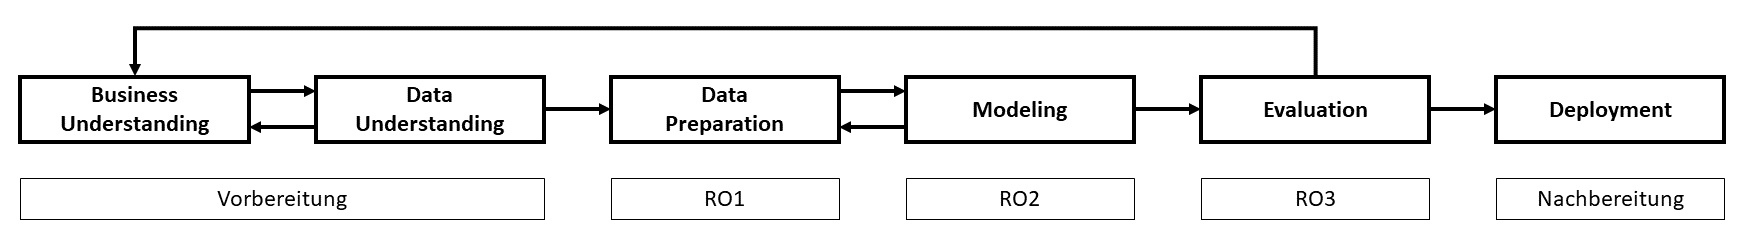
\includegraphics[width=\textwidth]{images/CRISP-DM}
    \caption{Phasen des CRISP-DM Prozessmodells nach \cite{Chapman2000} mit Zuordnung der Arbeitsphasen}\label{fig:crisp}
\end{figure}

Die ersten beiden Phasen \glqq Business Understanding\grqq{} und \glqq Data Understanding\grqq{} widmen sich der Vorbereitung der Arbeit. Die initiale Phase umfasst dabei die allgemeine Einarbeitung in das zugrundeliegende Thema und der Formulierung der Forschungsziele. Die darauffolgende Phase \glqq Data Understanding\grqq{} dient der Suche und Einsicht von für den weiteren Verlauf der Phasen relevanten Daten und, falls vorhanden, vorgefertigten Datensets (\textit{Anmerkung:} Es konnten keine passenden Datensets gefunden werden). Da Commits als Datenbasis zum Training der Klassifikatoren betrachtet werden, wird der überwiegende Teil der Suche nach Daten in Software-Repositories stattfinden, welche dem Versionierungssystem Git zugrunde liegen. Für die weiteren Phasen ist es von besonderer Bedeutung, den Aufbau der Daten sorgfältig zu untersuchen. Die dritte Phase \glqq Data Preparation\grqq{} kümmert sich um die Erstellung des featurebasierten Datensets und den dort hinführenden Prozessen. Diese Phase ist deckungsgleich mit den Anforderungen des ersten Forschungsziels. Zur Anwendung kommt das im vorherigen Schritt erstellte Datenset in der Phase \glqq Modeling\grqq{}. In dieser werden die auf Machine-Learning-Algorithmen basierenden Klassifikatoren mithilfe des Datensets trainiert. Diese Phase spiegelt somit die Erfüllung des zweiten Forschungsziels wider. Die fünfte Phase umfasst die Evaluation der Resultate der Tests der Klassifikatoren und deckt somit die Erfüllung des dritten Forschungsziels ab. Die Nachbereitung der Arbeit wird durch die Phase \glqq Deployment\grqq{} abgedeckt. Diese umfasst die Erstellung beziehungsweise Finalisierung der schriftlichen Ausarbeitung sowie das Erstellen der Abschlusspräsentation und der anschließenden Vorführung dieser im Rahmen des Kolloquiums.
Ferner sind in \autoref{fig:crisp} Rückpfeile zwischen einzelnen Phasen angegeben. So können beispielsweise Erkenntnisse im Rahmen der Phase Data Understanding zu offenen Fragestellungen führen, die die Phase des Business Understanding betreffen. Gleiches gilt für die Phase Modeling mit einem Rückpfeil zur Phase Data Preparation. Weiterhin können Erkenntnisse, die im Rahmen der Evaluationsphase gewonnen werden können, zuvor unbekanntes Wissen aus der ersten Phase erläutern.

\section{Aufbau der Arbeit}

Diese Ausarbeitung ist in sechs Kapitel unterteilt. \hyperref[introduction]{Kapitel 1}, welches mit diesem Abschnitt abgeschlossen wird, diente zur Einführung in das Thema der Masterarbeit. Ebenso stellte es die theoretischen Rahmenbedingungen der Arbeit vor. \hyperref[background]{Kapitel 2} dient zur Vermittlung von Basiswissen zu den grundlegenden Themenkomplexen dieser Ausarbeitung. Dazu wird zunächst die featurebasierte Softwareentwicklung vorgestellt, ehe dann die Machine-Learning-Klassifikation sowie die darauf aufbauende Fehlervorhersage erläutert werden. \hyperref[dataset-creation]{Kapitel 4} und \hyperref[training]{Kapitel 5} widmen sich der Auseinandersetzung des praktischen Teils dieser Masterarbeit in Form der Erstellung des featurebasierten Datensets sowie des Trainings der Machine-Learning-Klassifikatoren. Die Gegenüberstellung und Evaluation dieser Klassifikatoren erfolgt in \hyperref[evaluation]{Kapitel 5} inklusive eines Vergleiches zu einer nicht-featurebasierten klassischen Methode zur Fehlervorhersage. Eine abschließende Zusammenfassung sowie ein Ausblick auf weiterführende Projekte, die auf diese Masterarbeit aufbauen können, erfolgen in \hyperref[conclusion]{Kapitel 6}.

Zusätzlich wird die Ausarbeitung von zahlreichen Abbildungen und Tabellen zur verständlichen Verdeutlichung von Zusammenhängen ergänzt.

\cleardoublepage


% !TEX root = ../thesis.tex

\chapter{Hintergrund}
\label{background}

Zum besseren Verständnis der weiteren Verlaufs dieser Arbeit, dient dieses Kapitel zur Einführung in die zugrundeliegenden Themen. Dazu wird zunächst die featurebasierte Softwareentwicklung erläutert, ehe dann der Themenbereich des Machine Learnings vorgestellt wird. Dazu werden die Klassifikation und die Fehlervorhersage mittels Machine Learning erläutert. Unterstützt werden die Abschnitte von Grafiken zum besseren Verständnis der Zusammenhänge.
\\
\hrule

\section{Featurebasierte Softwareentwicklung}
\label{feat-develop}

Das zentrale Konzept hinter der featurebasierten Softwareentwicklung stellen sogenannte Soft-ware-Produktlinien dar. Wie bereits in der Einleitung erwähnt wurde, beschreiben Software-Produktlinien eine Menge von ähnlichen Softwareprodukten, welche eine gemeinsame Menge von Features sowie eine gemeinsame Codebasis besitzen und sich durch die Auswahl der verwendeten Features unterscheiden, sodass eine breite Variabilität innerhalb einer Produktlinie entstehen kann \cite{Apel2013,Thuem2014}.

Der zentrale Prozess der Generierung einer Software-Produktlinie ist in \autoref{fig:spl} dargestellt. Aufgeteilt wird dieser Prozess in das Domain Engineering und das Application Engineering. Im Rahmen des Domain Engineerings wird ein sogenanntes Variabilitätsmodell (Variability Model) erstellt, welches die wählbaren Features und Constraints für mögliche Selektionen beschreibt \cite{Apel2013}. Gängige Implementationstechniken für Features reichen von einfachen Lösungen durch Annotationen basierend auf Laufzeitparametern oder Präprozessor-Anweisungen bis hin zu verfeinerten Lösungen basierend auf erweiterten Programmiermethoden, wie zum Beispiel Aspektorientierung. In einigen dieser Implementierungstechniken wird jedes Feature wird als wiederverwendbares Domain Artifact modelliert und gekapselt, welches im Prozess des Application Engineerings in Form einer Konfiguration zusammen mit weiteren Features, im Hinblick auf die gewünschte Funktionalität der Software, ausgewählt werden kann. Ein Software Generator erzeugt dann die gewünschten Softwareprodukte basierend auf den bereits zuvor genannten Implementationstechniken für Features.

\begin{figure}[t]
    \centering
    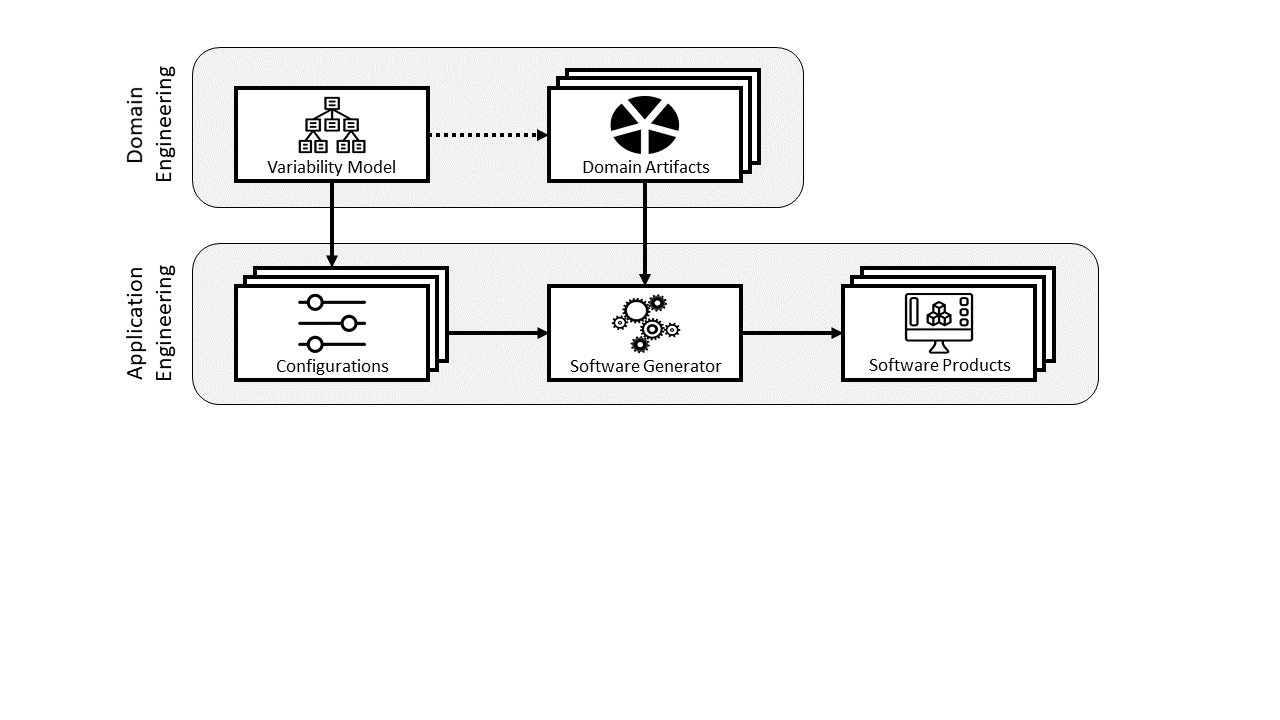
\includegraphics[width=\textwidth]{images/SPL}
    \caption{Generierung von Software-Produktlinien nach \cite{Thuem2014}\label{fig:spl}}
\end{figure}

Die in dieser Arbeit betrachtete Implementierungstechnik von Features basiert auf Anweisungen beziehungsweise Bedingungsdirektiven des C-Präprozessors. Die für diese Arbeit relevanten Direktiven lauten \texttt{\#IFDEF} und \texttt{\#IFNDEF}. Einfache Beispieleinsätze für beide Direktiven sind in \autoref{example1} und \autoref{example2} zu sehen. Sie wurden jeweils aus der wissenschaftlichen Literatur entnommen \cite{Medeiros2018,Preschern2019}. Die Direktive \texttt{\#IFDEF} leitet in \texttt{\#IFDEF} den Code des Features \texttt{\_\_unix\_\_} ein, welcher mit der Anweisung \texttt{\#ENDIF} endet. Der in den Zeilen 2 bis 6 angegebene Codeteil wird genau dann nur ausgeführt, wenn das Feature \texttt{\_\_unix\_\_} im Rahmen der Konfiguration des Softwareproduktes definiert beziehungsweise aktiviert ist \cite{Stallmann2016}. In diesem Fall wird die Bedingung der Direktive erfolgreich erfüllt \cite{Stallmann2016}. Sie schlägt fehl, wenn das Feature nicht definiert beziehungsweise aktiviert ist \cite{Stallmann2016}. Die Direktive \texttt{\#IFNDEF} wird für Code verwendet, der ausgeführt werden soll, wenn ein Feature nicht definiert ist. Im Falle des Beispiels in \autoref{example2} wird der in Zeile 3 angedeutete Code nur ausgeführt, wenn \texttt{NO\_XMALLOC} nicht aktiviert wurde.
Es besteht zudem die Möglichkeit, Features bzw. ihren Code zu verschachteln. Ein Beispiel dafür ist in \autoref{example3} angegeben. Es ist zu erkennen, dass sich der Code von \texttt{FEAT\_MZSCHEME} innerhalb der bedingten Gruppe von \texttt{USE\_XSMP} befindet. Der in Zeile 5 angedeutete Code kann somit nur ausgeführt werden, wenn \texttt{USE\_XSMP} aktiviert ist. Im Fall von Verschachtelung beendet ein \texttt{\#ENDIF} immer das nächstgelegene \texttt{\#IFDEF} oder \texttt{\#IFNDEF} \cite{Stallmann2016}. Es besteht zudem die Möglichkeit, Direktiven mittels \glqq und\grqq{} (\texttt{\&\&}, \texttt{and}) oder \glqq oder\grqq{} (\texttt{||}, \texttt{or}) zu erweiterten Bedingungen zu verknüpfen, die zudem Negation in Form des \texttt{!}-Operators (anstelle von \texttt{\#IFNDEF}) enthalten können \cite{Stallmann2016,Queiroz2015}. Dargestellt ist dies in \autoref{example4}.

\noindent\begin{minipage}{.45\textwidth}
\begin{lstlisting}[caption=Beispieleinsatz von \texttt{\#IFDEF} nach \cite{Preschern2019},frame=tlrb,language=C, label=example1]{example1}
#IFDEF __unix__
	#include "directorySelection.h"
	#include "directoryNames.h"
	void getDirectoryName(char* dirname) {
		getHomeDirectory(dirname);
	}
#ENDIF
\end{lstlisting}
\end{minipage}\hfill
\begin{minipage}{.45\textwidth}
\begin{lstlisting}[caption=Beispieleinsatz von \texttt{\#IFNDEF} nach \cite{Medeiros2018},frame=tlrb,language=C, label=example2]{example2}
int test = 1;
#IFNDEF NO_XMALLOC
	test = memory != NULL;
#ENDIF
if (test){
 // Lines of code here..
 } 
\end{lstlisting}
\end{minipage}

\noindent\begin{minipage}{.45\textwidth}
\begin{lstlisting}[caption=Beispiel eines verschachtelten Einsatzes von \texttt{\#IFDEF} nach \cite{Medeiros2018} ,frame=tlrb,language=C, label=example3, firstnumber=1]{example3}
bool time = msec > 0;
#IFDEF USE_XSMP
	time = time && xsmp_icefd != -1;
	#IFDEF FEAT_MZSCHEME
 		time = time || p_mzq > 0;
	#ENDIF
#ENDIF
if (time)
 gettime(&start_tv);
\end{lstlisting}
\end{minipage}\hfill
\begin{minipage}{.45\textwidth}
\begin{lstlisting}[caption=Beispiele von erweiterten Bedingungen nach \cite{Queiroz2015},frame=tlrb,language=C, label=example4, firstnumber=1]{example4}
#IFDEF FEATURE_A && FEATURE_B
	(...)
#ENDIF
(...)
#IFDEF !FEATURE_A && FEATURE_C
	(...)
#ENDIF
\end{lstlisting}
\end{minipage}

Die in den Listings gezeigten Beispiele zeigen jeweils nur den Featurecode in einer Methode beziehungsweise in einer Datei. Fragmente des Featurecodes erstrecken sich jedoch nicht nur möglicherweise mehrfach über eine Datei sondern über mehrere Dateien - der Featurecode ist somit verstreut (englisch: code scattering), um eine Funktionalität des Features in der Gesamtheit der Software zu ermöglichen. Ein Defekt innerhalb eines Fragmentes des Featurecodes kann allerdings dazu führen, dass die gesamte Funktionalität des Features beeinträchtigt oder unterbunden wird, da der Fehler übergreifend wirkt (englisch: cross-cutting). Ebenfalls kann ein solcher Fehler dazu führen, dass die Funktionalität des gesamten Sourcecodes beeinträchtigt wird.

\section{Machine-Learning-Klassifikation}
\label{classification}

Das Themengebiet des Machine Learnings (ML) ist in zwei Teilgebiete unterteilt - das unüberwachte ML (englisch: unsupervised ML) und das überwachte ML (englisch: supervised ML). Die Methoden in diesen Teilgebieten verfolgen unterschiedliche Ziele. Im Rahmen des unüberwachten ML werden Prozesse durchgeführt, welche dazu dienen, die Struktur einer unbekannten Eingabemenge an Daten zu erlernen und anschließend zu repräsentieren \cite{Sammut2017}. Eine gängige Anwendung des unüberwachten ML ist das Clustering. Das überwachte ML beschreibt wiederum einen Prozess, welcher beabsichtigt, Vorhersagen über unbekannte Eingabedaten auf Basis der Erlernung einer Abbildungsfunktion zu treffen \cite{Sammut2017}. Die Attribute \glqq unüberwacht\grqq{} und \glqq überwacht\grqq{} erhalten die Methoden aufgrund ihrer Art des Lernens. In der Anwendung des unüberwachten ML werden die Eingabedaten erfasst, gegebenenfalls vorverarbeitet, um dann auf deren Basis ein Modell zu erlernen, welches die Darstellung beziehungsweise Repräsentation der Eingabedaten bestimmt \cite{Alpaydin2010}. Auf der anderen Seite, wird unter Anwendung des überwachten ML, ein Modell auf Basis eines sogenannten \glqq gelabelten\grqq{} (beschrifteten) Datensatzes durch Merkmalsextraktion in Form von Attributen und Lernen auf der Grundlage der extrahierten Merkmale erstellt \cite{Alpaydin2010}. Der Datensatz, welcher zur Erlernung verwendet wird, wird im gängigen Sprachgebrauch des Machine Learning Datenset (englisch: dataset) genannt. Das aus der Erlernung resultierende Modell wird Klassifikator (englisch: classifier) genannt. Gängige Anwendungen des überwachten ML sind Regression und Klassifikation. In dieser Arbeit kommt die Klassifikation als Anwendung des überwachten ML zum Einsatz. Der grundlegende Prozess der Machine-Learning-Klassifikation ist in \autoref{fig:ml} anhand eines Beispiels dargestellt.

\begin{figure}[t]
    \centering
    \captionsetup{justification=centering,margin=2cm}
    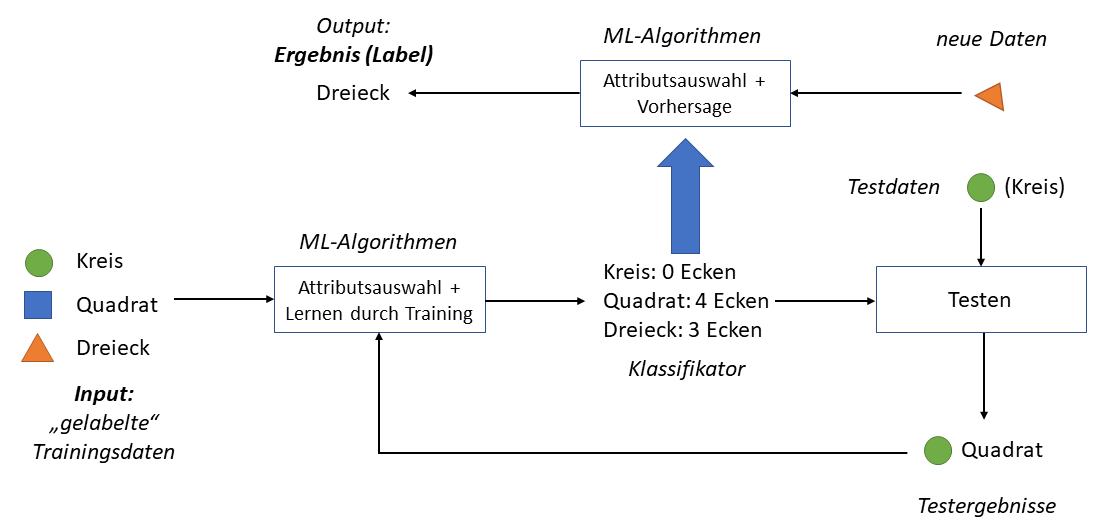
\includegraphics[width=\textwidth]{images/ML}
    \caption{Allgemeiner Prozess des überwachten Machine Learnings dargestellt anhand eines Beispiels (vereinfacht)}\label{fig:ml}
\end{figure}

Die Abbildung zeigt den Prozess des überwachten Machine Learnings anhand des Beispiels der Erlernung eines Klassifikators zur Erkennung beziehungsweise Vorhersage von geometrischen Formen. Der Prozess beginnt mit den \glqq gelabelten\grqq{} Eingabedaten (A). Die Werte der Label (kategorial oder numerisch) stellen dabei die zu vorhersagende Zielklasse dar. In diesem Falle bilden die Namen der geometrischen Formen die Label als kategorischen Wert. Die Rohdaten der Eingabemenge bestehen aus den geometrischen Formen selbst. Beide Datenmengen bilden das Datenset. Um nun einen Klassifikator anlernen zu können, müssen Merkmale der Eingangsdaten ausgewählt werden, anhand derer diese identifiziert werden können (B). Diese zu identifizierenden Charakteristika der Daten werden Attribute genannt. Diese Attribute können bereits vor dem Erlernen festgelegt werden oder automatisiert extrahiert werden. Im vorliegenden Fall wurde die Metrik \glqq Anzahl der Ecken der geometrischen Formen\grqq{} als Attribut zur Erlernung ausgewählt. Das Ergebnis ist der fertig trainierte Klassifikator, welcher das erlernte Wissen auf neue Daten abbilden kann (C). Ein Teil des Datensets wird in der Regel verwendet, um den Klassifikator nach dessen Erstellung zu testen (D). Die in der Regel verwendeten Verhältnisse (englisch: Split-Ratio) zwischen Trainings- und Testdaten betragen 80:20 (basierend auf dem Paretoprinzip) oder 75:25 (zum Beispiel \cite{Queiroz2016}). Diese Testdaten werden dem Klassifikator als Eingabemenge zur Klassifikation ohne Label zur Verfügung gestellt. Die Label sollten jedoch nicht verworfen werden, da sie als Vergleichsgrundlage für die Verhersageperformanz des Klassifikators dienen. Sie bilden die sogenannte \glqq Ground Truth\grqq{} (deutsch: Grundwahrheit). Dazu werden die vom Klassifikator vorhergesagten Label mit denen der Ground Truth verglichen. Sollte dieser Vergleich ergeben, dass die Label große Abweichungen zeigen, so kann der Klassifikator erneut erlernt werden mit anderen Attributen oder einer veränderten Split-Ratio. Erfüllt der Klassifikator die Anforderungen an die Performanz der Vorhersagen, so ist dieser bereit Vorhersagen auf Basis neuer Eingabedaten zu treffen (E). Dazu müssen von den neuen Daten die Attribute ermittelt werden. Auf Basis dieser trifft der Klassifikator die Vorhersage und liefert als Ausgabe das Label des Wertes der Zielklasse. Im Voraus des Testens mit den Testdaten (D) werden in manchen Fällen zudem sogenannte Validierungsdaten verwendet. Dabei handelt es sich um eine eigenständige Teilmenge der Trainingsdaten, welche verwendet wird, um die Klassifikatoren nach jeder Erlernung zu evaluieren, um die Auswahl der Attribute hinsichtlich der Performanz auf Eignung zu prüfen \cite{Sammut2017}. Die Anwendung der Testdaten erfolgt dann im Anschluss.

Der in \autoref{fig:ml} dargestellte Klassifikator stellt einen multinomiellen oder multi-class Klassifikator dar, da er zu drei oder mehr Werten der Zielklasse zuordnen kann \cite{Sammut2017}. Für viele praktische Anwendungen genügt jedoch ein binärer Klassifikator, welcher Vorhersagen zu zwei Werten der Zielklasse trifft. Dies trifft auch auf die Klassifikatoren dieser Arbeit zu.

\section{Fehlervorhersage mittels Machine Learning}

Der Hintergrund der Fehlervorhersage mittels Machine Learning basiert auf dem zuvor vorgestellten Konzept des überwachten Machine Learnings. Als Grundlage dienen dabei meist Daten, die aus Software-Repositories entnommen beziehungsweise extrahiert werden. Viele Studien und wissenschaftliche Arbeit setzen jedoch auch auf vorgefertigte Datensets, wie zum Beispiel von der NASA oder von Eclipse \cite{Son2019}. Die zugehörigen Label der Datensets lauten in der Regel \glqq fehlerfrei\grqq{} und \glqq defekt\grqq{} und können auf verschiedene Weisen ermittelt werden. Eine gängige Methode ist die Identifizierung von korrektiven und fehlereinführenden Commits als Entscheidungsgrundlage für das Label. Die üblichen Vorgehensweisen setzen auf die Einbindung von Bugtracking-Systemen oder die Analyse von Commit-Nachrichten zur Identifizierung der korrektiven Commits \cite{Queiroz2016,Zimmermann2007}. Fehlereinführende Commits können anschließend unter Verwendung von Git-Kommandos oder durch die Anwendung des sogenannten SZZ-Algorithmus ermittelt werden. Dieser Algorithmus wird in dieser Arbeit verwendet und in \hyperref[szz-def]{Abschnitt 3.2} erläutert. Auf Basis dieser Daten werden die Attribute bestimmt. Dabei handelt sich sich in der Regel um Metriken, die entweder die Charakteristika des Sourcecodes (Codemetriken) oder Aktivitäten und Prozesse im Bezug auf Software-Repositories (Prozessmetriken) beschreiben \cite{Son2019,Rahman2013}. Mithilfe dieser Attribute werden die Klassifikatoren erlernt. Eine Studie, welche 156 wissenschaftliche Arbeiten zum Thema der Fehlervorhersage mittels Machine Learning analysierte, ergab, dass besonders Entscheidungsbaum-basierte, Bayessche Verfahren, Regression und künstliche neuronale Netze als Klassifikationsalgorithmen zur Anwendung kommen \cite{Son2019}. Diese Algorithmen wurden unter anderem auch in dieser Arbeit verwendet. Erläuterungen können in \hyperref[algorithms]{Abschnitt 4.1} gefunden werden. Die fertig erlernten Klassifikatoren können dann auf Basis neuer Daten Vorhersagen zum Zustand einer Software treffen. Die Vorhersagen beruhen in der Regel auf defekte Dateien im Umfeld von Commits oder Releases.

Als Beispiel für zwei konkrete Anwendungen von Machine Learning gestützter Fehlervorhersage werden im Folgenden zwei wissenschaftliche Arbeiten vorgestellt. Die erste Arbeit \glqq Comparative Analysis of the Efficiency of Change Metrics and Static Code Attributes for Defect Prediction\grqq{} von Moser et al. \cite{Moser2008} stellt eine Methodik zur dateibasierten Fehlervorhersage vor. Die zweite Arbeit \glqq Towards Predicting Feature Defects in Software Product Lines\grqq{} von Queiroz et al. \cite{Queiroz2016} knüpft an den zuvor vorgestellten Ansatz der Software-Features an. Beide Literaturquellen werden im weiteren Verlauf dieser Arbeit eine Rolle spielen, die im jeweiligen Abschnitt erläutert wird.

\subsection*{Dateibasierte Fehlervorhersage}
Das Beipsiel zur dateibasierten Fehlervorhersage stammt aus einer wissenschaftlichen Arbeit von Moser et al. \cite{Moser2008}. Sie widmet sich einer vergleichenden Analyse von zwei verschiedenen Mengen von Metriken zur dateibasierten Fehlervorhersage mittels Methoden des Machine Learnings. Die Zuordnung erfolgt in \glqq defekt\grqq{} und \glqq defekt-frei\grqq. Als Datenbasis dient ein vorgefertigtes Datenset von Eclipse. Auf Basis dieses Datensets wurden \glqq produktbasierte\grqq{} Metriken (Codemetriken) und Prozessmetriken berechnet. Zur Anwendung kamen die Klassifikationsalgorithmen logistische Regression, Na\"{\i}ve Bayes und Entscheidungsbäume. Die Prozessmetriken stellen eine Besonderheit dieser Arbeit dar, da sie in dieser Arbeit zum ersten Mal näher betrachtet und auf ihre Eignung als Attribute zur Erlernung der Klassifikatoren erörtert wurden. Die Metriken berechneten unter anderem die Anzahl der Änderungen an einer Datei, die Anzahl der Autoren einer Datei, die Anzahl der hinzugefügten oder entfernten Zeilen einer Datei oder das Alter einer Datei. Das Resultat der Arbeit lautet, dass Prozessmetriken effektiver zur Fehlervorhersage genutzt werden können als Codemetriken.

Im Rahmen der Evaluation der für diese Arbeit erlernten featurebasierten Klassifikatoren wird ein zusätzliches dateibasiertes Datenset erstellt, welches auf diesen Prozessmtriken basiert und zum Performanzvergleich hinsichtlich der neuen featurebasierten Betrachtung hinzugezogen wird. Die vollständige Liste der Metriken ist in \hyperref[classic-eval]{Abschnitt 5.3} aufgeführt.

\subsection*{Featurebasierte Fehlervorhersage}

Das Beispiel zur featurebasierten Fehlervorhersage stammt aus einer wissenschaftlichen Arbeit von Queiroz et al. \cite{Queiroz2016}. Bei dieser Fallstudie handelt es sich um die erste und bisher einzige Arbeit über Fehlervorhersage mit Bezug zu Software-Features. Sie stellt somit für diese Masterarbeit eine bedeutende literarische Grundlage dar. Der Ablauf des von Queiroz et al. angewandten Prozesses zur Erstellung eines featurebasierten Datensets und dessen Anwendung zur Erlernung von Klassifikatoren orientiert sich am zuvor vorgestellten allgemeinen Prozess des überwachten Machine Learnings.

Die Erläuterung des Beispiels erfolgt anhand von zwei Abbildungen, welche den in der Arbeit von Queiroz et al. vorgestellten Prozess in zwei Teilen visualisieren. Der erste Teil ist in \autoref{fig:ml1} dargestellt.

\begin{figure}[t]
    \centering
    \captionsetup{justification=centering}
    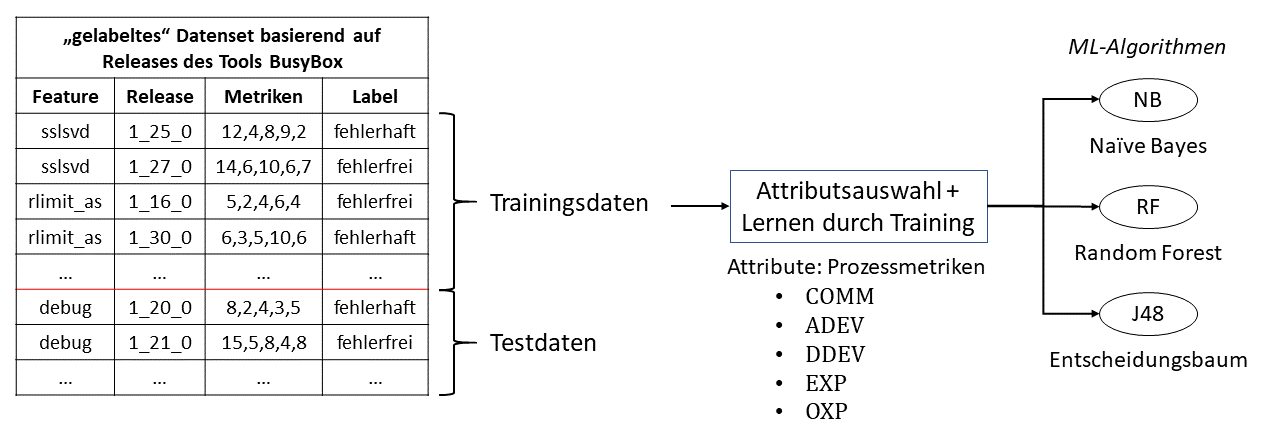
\includegraphics[width=\textwidth]{images/ML1}
    \caption{Teil 1: Featurebasierter Prozess des überwachten Machine Learnings nach \cite{Queiroz2016}}\label{fig:ml1}
\end{figure}

\subsubsection*{Datenset}

Die Datenbasis des Datensets bilden historische Commits des UNIX-Toolkits BusyBox\footnote{\url{https://busybox.net/}}, dessen Quellcode frei verfügbar in einem Git-Repository\footnote{\url{https://git.busybox.net/busybox/}} eingesehen und von dort geklont werden kann. Diese Commits wurden wiederum ihren entsprechenden Releases zugeordnet, welche auf der vergebenen Tag-Struktur des Repositories beruhen. Ferner wurden aus den Diffs der Commits die dort bearbeiteten Features extrahiert und anschließend zusammen mit den Release-Informationen in einer MySQL-Datenbank gespeichert. Zusätzlich enthält jeder Datenbankeintrag aggregierte Werte von fünf auf das Feature und den Release bezogenen Prozessmetriken (Erläuterung folgt) sowie das binäre Label, ob ein Feature in einem Release fehlerhaft oder fehlerfrei war. Ein Feature gilt in einem Release als fehlerhaft, sofern in einem Commit des darauffolgenden Releases ein fehlerbehebender Commit bezüglich des Features festgestellt werden konnte. Dies geschieht über die Analyse der Commit-Nachrichten. Sofern eine Commit-Nachricht die Begriffe \glqq bug\grqq{} (Fehler), \glqq error\grqq{} (schwerwiegender Fehler), \glqq fail\grqq{} (fehlschlagen) oder \glqq fix\grqq{} (beheben) enthält, werten die Autoren des Papers den Commit als fehlerbehebend. Alternative Methoden zur Durchführung dieser Analyse bestehen aus der Eindbindung von Daten aus Bug-Tracking-Systemen, die häufig an Software-Repositories angebunden sind, sowie aus der Anwendung des sogenannten SZZ-Algorithmus, welcher in dieser Arbeit verwendet wurde und in \hyperref[szz-def]{Abschnitt 3.2} erläutert wird \cite{Sliwerski2005,Zimmermann2007}. Wie im Rahmen des überwachten Machine Learning üblich, wird das Datenset in Trainings- und Testdaten in einem Verhältnis von 75:25 geteilt. 

\subsubsection*{Metriken und Klassifikation}

Die Trainingsdaten werden dann den Klassifikatoren zur Erlernung zur Verfügung gestellt. Als Attribute dienen fünf Prozessmetriken mit spezifischer Betrachtung von Software-Features. Einen Überblick über die Beschreibungen dieser gibt \autoref{tab:metrics-rodrigo}. Als Klassifikationsalgorithmen wurden Na\"{\i}ve Bayes, Random Forest und J48-Entscheidungsbäume gewählt.

\begin{table}[t]
\centering
\caption{Übersicht der von \cite{Queiroz2016} verwendeten Prozessmetriken}
\label{tab:metrics-rodrigo}
\begin{tabular}{|c|l|} 
\hline
\textbf{Metrik}  & \textbf{Beschreibung}  \\ 
\hline
COMM & \begin{tabular}[c]{@{}l@{}}Anzahl der Commits, die in einem Release dem betreffenden \\ Feature gewidmet sind. \end{tabular} \\ 
\hline
ADEV & \begin{tabular}[c]{@{}l@{}}Anzahl der Entwickler, die das betreffende Feature\\in einem Release bearbeitet haben. \end{tabular} \\ 
\hline
DDEV & \begin{tabular}[c]{@{}l@{}}kummulierte Anzahl der Entwickler, die das betreffende Feature\\in einem Release bearbeitet haben. \end{tabular} \\ 
\hline
EXP & \begin{tabular}[c]{@{}l@{}}Geometrisches Mittel der \glqq Erfahrung\grqq{} aller Entwickler, die am \\ betreffenden Feature in einem Release gearbeitet haben. \end{tabular} \\ 
\hline
OEXP & \begin{tabular}[c]{@{}l@{}}\glqq Erfahrung\grqq{} des Entwicklers, der am meisten zum betreffenden \\ Feature in einem Release beigetragen hat. \end{tabular} \\ 
\hline
\multicolumn{2}{|c|}{\begin{tabular}[c]{@{}c@{}}Erfahrung ist definiert als Summe der geänderten, gelöschten\\oder hinzugefügten Zeilen im zugehörigen Release. \end{tabular}} \\
\hline
\end{tabular}
\end{table}

\begin{figure}[t]
    \centering
    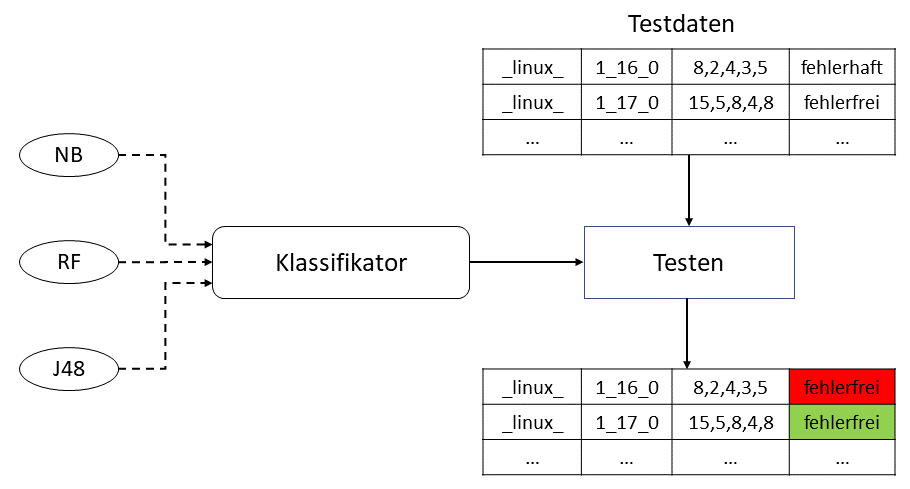
\includegraphics[width=0.8\textwidth]{images/ML2}
    \caption{Teil 2: Featurebasierter Prozess des überwachten Machine Learnings nach \cite{Queiroz2016}}\label{fig:ml2}
\end{figure}

\subsubsection*{Test der Klassifikatoren}

Wie in \autoref{fig:ml2} dargestellt ist, wird für jeden Klassifikationsalgorithmus ein Klassifikator erstellt, welcher anschließend getestet und evaluiert wird. Dazu werden die jeweiligen Klassifikatoren auf das Testdatenset angewendet, ohne jedoch die Werte der Zielklassen mit anzugeben. Diese werden im Anschluss an den Klassifikationsvorgang mit den vorhergesagten Werten auf Übereinstimmung verglichen. Anhand dieses Vergleiches können die Genauigkeit sowie weitere Metriken zur Bewertung der Leistung der Klassifikatoren gemessen werden. Eine Übersicht von Evaluationsmetriken kann in \hyperref[eval-metrics]{Abschnitt 5.2.1} gefunden werden.

Die so erstellten Klassifikatoren können dann zur Vorhersage von neuen Daten genutzt werden. Dazu müssen die fünf zuvor genannten Prozessmetriken der neuen Daten berechnet werden. 

\cleardoublepage


% !TEX root = /doc.tex

\section{Methodology}

\subsection{Creation of Dataset}

The data set forms the basis for the training of the machine learning classifiers and is created specifically for this work based on commits from 12 feature-based software projects. The software projects are selected on the basis of previous use in scientific literature \cite{Hunsen2015,Liebig2010,Queiroz2015,Queiroz2016}. The software projects used for this thesis are listed in \autoref{tab:tools} together with their purpose and data sources.

\begin{table}[ht]
\centering
\caption{Used software projects}
\label{tab:tools}
\resizebox{\linewidth}{!}{%
\begin{tabular}{|l|l|l|} 
\hline
 \textbf{Project}  & \textbf{Purpose}  & \textbf{Data source}    \\ 
\hline
\textbf{Blender}   & 3D modelling tool & GitHub mirror           \\ 
\hline
\textbf{Busybox}   & UNIX toolkit      & Git repository          \\ 
\hline
\textbf{Emacs}     & text editor       & GitHub mirror           \\ 
\hline
\textbf{GIMP}      & graphics editor   & GitLab repository       \\ 
\hline
\textbf{Gnumeric}  & spreadsheet       & GitLab repository       \\ 
\hline
\textbf{gnuplot}   & plotting tool     & GitHub mirror           \\ 
\hline
\textbf{Irssi}     & IRC client        & GitHub repository       \\ 
\hline
\textbf{libxml2}   & XML parser        & GitLab repository       \\ 
\hline
\textbf{lighttpd}  & web server        & Git repository          \\ 
\hline
\textbf{MPSolve}   & polynom solver    & GitHub repository       \\ 
\hline
\textbf{Parrot}    & virtual machine   & GitHub repository       \\ 
\hline
\textbf{Vim}       & text editor       & GitHub repository       \\ 
\hline
\end{tabular}
}
\end{table}

To get the commit data of the software projects the Python library PyDriller\footnote{\href{https://github.com/ishepard/pydriller}{https://github.com/ishepard/pydriller}} was used \cite{Spadini2018}. This allows easy data extraction from Git repositories to obtain commits, commit messages, developers, diffs, and more (called "metadata" in the following). The URLs to the Git repositories of the software projects were used as input for the specially created Python scripts for receiving the commit metadata. Furthermore, the metadata was divided into commits per release. This was made possible by specifying release tags in the PyDriller code, based on the tag structure of Git repositories. For each modified file within a commit and a release, the following metadata was retrieved using PyDriller:

\begin{itemize}
\item commit hash (unique identifier of a commit)
\item commit author
\item commit message
\item filename
\item lines of code
\item cyclomatic complexity
\item number of added lines
\item number of removed lines
\item diff (changeset)
\end{itemize}

The data obtained in this way was stored in a MySQL database after retrieval. For each software project, a separate table was created in which, in addition to the metadata above, the name of the software project and the release numbers associated with the commits were stored. Each modified file of a commit receives one row of the database tables. The further construction of the data set is divided into several phases of data processing and optimization.

The first phase consists of extracting the features involved in a modified file. This was done by using a Python script to identify the preprocessor statements \texttt{\#IFDEF} and \texttt{\#IFNDEF} in the diffs of the modified files, and then saving the string following the directives as a feature until the end of the line of code. The identification was done using regular expressions. The features identified per file are stored in an additional column in the respective MySQL tables. In case a feature is identified after the \texttt{\#IFNDEF} directive, the feature is stored with a preceding "not". It will be saved as a separate feature, along with its non-negated form. Combinations of features are stored in their identified form. If no feature could be identified, "\texttt{none}" is saved accordingly.

This way of identification has some obstacles. In some C programming paradigms, it is common to include header files in the source code using preprocessor directives, so that they appear to be features. However, these "header features", as they will be referred to later, should be ignored as they do not create variability throughout the source code. In general, these header features are identifiable by their naming in the form of an appended \texttt{\_h\_} to the feature name, such as \texttt{featurename\_h\_}. This appended part allows the header features to be identified and filtered out using regular expressions. It is also possible that "wrong" features can be identified. Examples of this can come from \texttt{\#IFDEFs} used in comments. Such false features were removed in a manual review of the identified features and replaced with "\texttt{none}".

The next phase of processing consists of identifying corrective commits. A common method used for this, and one used in this paper, is to analyze commit messages for the presence of certain keywords \cite{Zimmermann2007}. The keywords are "bug," "bugs," "bugfix," "error," "fail," "fix," "fixed," and "fixes. The analysis was carried out by means of a Python script using simple methods of Natural Language Processing (NLP). Identification was limited to the first line of each commit message. The results were stored in another column of the MySQL tables (true = corrective, false = not corrective).

The search for corrective commits is followed by an analysis for commits that introduced bugs. A PyDriller implementation of the SZZ algorithm according to Sliwerski, Zimmermann and Zeller was used \cite{Sliwerski2005,Spadini2018}. This algorithm allows to find commits that introduce bugs in locally stored software repositories \cite{Borg2019}. It requires that the corrective commits have already been identified, as they serve as the algorithm's input \cite{Borg2019}.

An overview of the number of corrective and bug-introducing commits and the number of features identified per software project is given in \autoref{tab:tools-values2}.

\begin{table}[ht]
\centering
\caption{Number of corrective and bug-introducing commits and number of identified features}
\label{tab:tools-values2}
\resizebox{\linewidth}{!}{%
\begin{tabular}{|l|r|r|r|} 
\hline
 \textbf{Project} & \textbf{\#corrective} & \textbf{\#bug-introducing} & \textbf{\#features}   \\ 
\hline
Blender           & 7.760                 & 3.776                      & 1.400                 \\ 
\hline
Busybox           & 1.236                 & 802                        & 628                   \\ 
\hline
Emacs             & 4.269                 & 2.532                      & 718                   \\ 
\hline
GIMP              & 1.380                 & 854                        & 204                   \\ 
\hline
Gnumeric          & 1.498                 & 1.191                      & 637                   \\ 
\hline
gnuplot           & 854                   & 1.215                      & 558                   \\ 
\hline
Irssi             & 52                    & 22                         & 9                     \\ 
\hline
libxml2           & 324                   & 88                         & 200                   \\ 
\hline
lighttpd          & 1.078                 & 929                        & 230                   \\ 
\hline
MPSolve           & 151                   & 211                        & 54                    \\ 
\hline
Parrot            & 3.109                 & 3.072                      & 397                   \\ 
\hline
Vim               & 371                   & 696                        & 1.158                 \\ 
\hline
\end{tabular}
}
\end{table}

A real example from the data of the Vim software project, showing the diffs of a corrective (A) and a bug-introducing (B) commit to a feature \texttt{FEAT\_TEXT\_PROP}, is shown in \autoref{fig:bug-example}. The section of the diff shows that the method call \texttt{vim\_memset} has been replaced with different arguments. According to the associated commit message, the original method call caused a "memory access error". This commit was identified as corrective because the commit message contains the keyword "error". The corresponding entry in Vim's main table thus gets the value \texttt{true} in the "corrective" column. Using the SZZ algorithm, specifying the commit hash of the corrective commit, the error-initiating commit (B) of the file concerned. In its portion of the diff, you can see that this commit has put the feature \texttt{FEAT\_TEXT\_PROP} in the file with the incorrect method call. As a result, it is assigned the value \texttt{true} in the "bug\_introducing" column in the main table.

\begin{figure*}[ht]
    \centering
    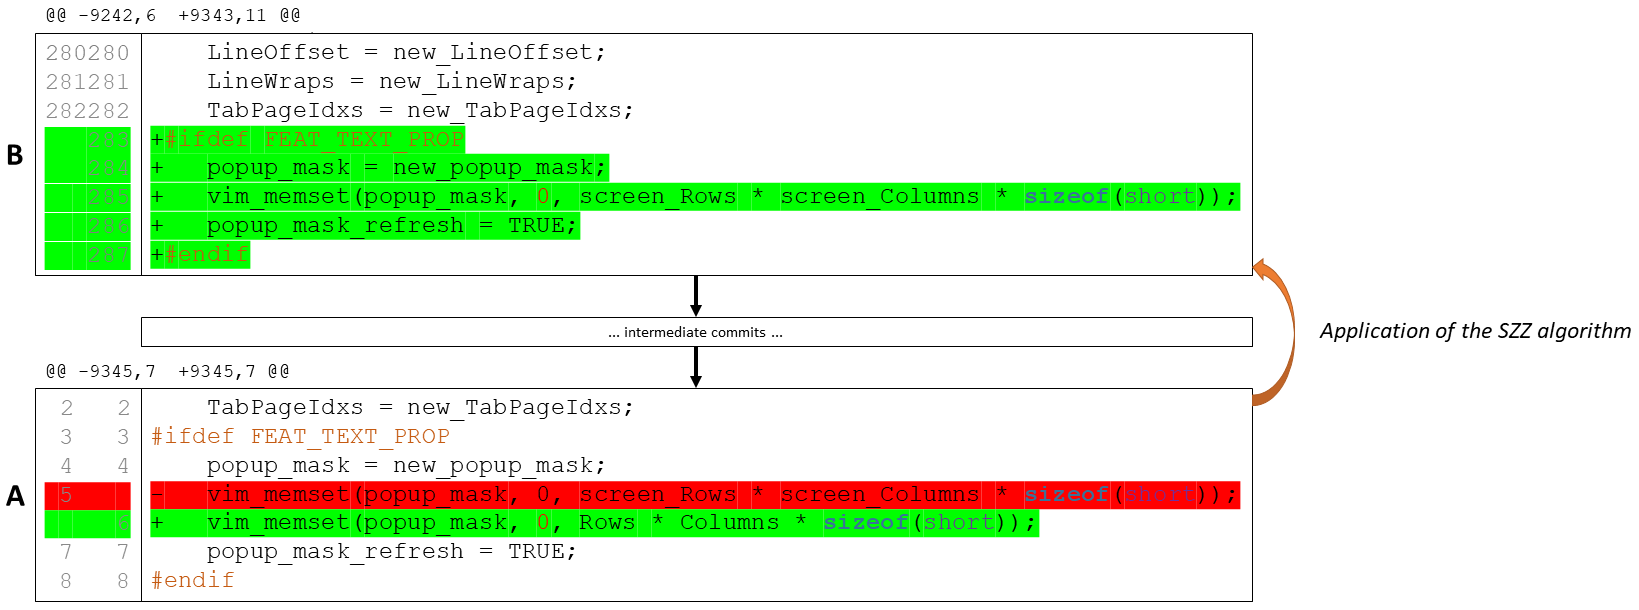
\includegraphics[width=\textwidth]{Bug_example_real}
    \Description{Real example of a defect.}
    \caption{Real example of a defect with corrective (A) and bug-introducing (B) commit\label{fig:bug-example}}
\end{figure*}


\subsection{Selection of Metrics}

As already mentioned, attributes are used to train the machine learning classifiers. In this scenario, so-called metrics are used as attributes. Metrics are numerical values that quantify properties of a software project. In this case, the metrics are divided into the usual categories code metrics and process metrics and each is calculated using the existing raw data of the main tables \cite{Rahman2013}. Code metrics are used to measure properties of source code, such as "size" or complexity \cite{Rahman2013}. Process metrics are used to measure properties that can be discussed using metadata from software repositories \cite{Rahman2013}. Examples include the number of changes made to a particular file or the number of active developers on a project. For this work, eleven feature-based metrics were calculated, divided into seven process and four code metrics. Five of the process metrics were taken from scientific papers \cite{Rahman2013,Queiroz2016}. The other six metrics were calculated based on the commit metadata obtained from PyDriller. A list of the eleven metrics and their descriptions can be found in \autoref{tab:metrics}. The individual metrics were calculated either directly using SQL queries or combined using SQL queries and calculations by a Python script.

In view of the evaluation of the feature-based dataset that follows in the next section, two additional datasets were created to make the impact of the feature-based metrics on the classifiers' predictions comparable. Both further data sets follow a classical file-based approach as it is common in machine learning based error detection and are based on the methodology developed by Moser et al. \cite{Moser2008}. The 17 process metrics of this scientific work were also adopted and are listed in \autoref{tab:metrics-moser}. A visualization to distinguish the three data sets is shown in \autoref{fig:dataset}.

\begin{table*}[ht]
\centering
\caption{Overview of used metrics}
\label{tab:metrics}
\resizebox{\linewidth}{!}{%
\begin{tabular}{|>{\hspace{0pt}}p{0.027\linewidth}|>{\hspace{0pt}}p{0.312\linewidth}|>{\hspace{0pt}}p{0.592\linewidth}|>{\hspace{0pt}}p{0.062\linewidth}|} 
\cline{2-4}
\multicolumn{1}{>{\hspace{0pt}}p{0.027\linewidth}|}{}  & \textbf{Metric}                                         & \textbf{Description}                                                                                                                                                                                                                                                                              & \textbf{Source}   \\ 
\hline
\multirow{7}{0.027\linewidth}{\hspace{0pt}\rotatebox[origin=c]{90}{Process metrics}\textbf{}} & Number of commits                                & Number of commits associated with the feature/file in a release.                                                                                                                                                                                                                                  & \cite{Queiroz2016}              \\ 
\cline{2-4}
                                                       & Number of active developers                       & Number of developers who have edited (changed, deleted or added) \par{}the feature / file within a release                                                                                                                                                                                        & \cite{Queiroz2016}              \\ 
\cline{2-4}
                                                       & Number of distinct developers                    & Cumultative number of developers who have edited (changed, deleted or added) \par{}the feature / file within a release                                                                                                                                                                            & \cite{Queiroz2016}              \\ 
\cline{2-4}
                                                       & Experience of all develepoers                     & geometric mean of the experience of all developers who have edited \par{}(changed, deleted or added) the feature / file within a release.\textasciitilde{}\par{}Experience is defined as the sum of the changed, deleted or added \par{}lines in the commits associated with the feature / file.  & \cite{Queiroz2016}              \\ 
\cline{2-4}
                                                       & Experience of the most involved developers & Experience of the developer who has edited (changed, deleted or added) \par{}the feature / file most often within a release. Experience is defined as the \par{}sum of changed, deleted, or added lines in the commits associated with the \par{}feature/file.                                    & \cite{Queiroz2016}              \\ 
\cline{2-4}
                                                       & Degree of modifications & Number of edits (change, removal, extension) of the feature / file within a release.                                                                                                                                                                                                              & *                 \\ 
\cline{2-4}
                                                       & Scope of modifications & Number of edited features / files within a release (feature or file overlapping value). \par{}Idea: The more features / files have been edited in a release, \par{}the more error-prone they seem to be.                                                                                          & *                 \\ 
\hline
\multirow{4}{0.027\linewidth}{\hspace{0pt}\rotatebox[origin=c]{90}{Code metrics}\textbf{}} & Lines of code                                    & Average number of lines of code of the files associated with the feature /\par{}\textasciitilde{}file within a release.                                                                                                                                                                           & *                 \\ 
\cline{2-4}
                                                       & Cyclomatic Complexity & Average cyclomatic complexity of the files associated with the feature / \par{}file within a release.                                                                                                                                                                                             & *                 \\ 
\cline{2-4}
                                                       & Number of added lines & Average number of lines of code added to the files associated with \par{}the feature / file within a release.                                                                                                                                                                                     & *                 \\ 
\cline{2-4}
                                                       & Number of removed lines                         & Average number of lines of code deleted from the files associated \par{}with the feature / from the file within a release                                                                                                                                                                         & *                 \\ 
\hline
\multicolumn{4}{|>{\centering\arraybackslash\hspace{0pt}}p{0.993\linewidth}|}{\textit{* These values were calculated based on the metadata obtained with PyDriller.}\par{}\textit{Feature-level metrics were calculated based on the metadata of the underlying files.}}                                                                                                                                                                 \\
\hline
\end{tabular}
}
\end{table*}

\begin{table}
\centering
\caption{Process metrics according to \cite{Moser2008}}
\label{tab:metrics-moser}
\resizebox{\linewidth}{!}{%
\begin{tabular}{|l|l|} 
\hline
\textbf{Metric}   & \textbf{Description}                                                      \\ 
\hline
REVISIONS         & Number of revisions of a file.                                            \\ 
\hline
REFACTORINGS      & Number of times a file has been refactored.                               \\ 
\hline
BUGFIXES          & Number of times a file was involved in bug-fixing.                        \\ 
\hline
AUTHORS           & Number of distinct authors that checked a file into the repository.       \\ 
\hline
LOC\_ADDED        & Sum over all revisions of the lines of code added to a file.              \\ 
\hline
MAX\_LOC\_ADDED   & Maximum number of lines of code added for all revisions.                  \\ 
\hline
AVE\_LOC\_ADDED   & Average lines of code added per revision.                                 \\ 
\hline
LOC\_DELETED      & Sum over all revisions of the lines of code deleted from a file.          \\ 
\hline
MAX\_LOC\_DELETED & Maximum number of lines of code deleted for all revisions.                \\ 
\hline
AVE\_LOC\_DELETED & Average lines of code deleted per revision.                               \\ 
\hline
CODECHURN         & Sum of (added lines of code – deleted lines of code) over all revisions.  \\ 
\hline
MAX\_CODECHURN    & Maximum CODECHURN for all revisions.                                      \\ 
\hline
AVE\_CODECHURN    & Average CODECHURN per revision.                                           \\ 
\hline
MAX\_CHANGESET    & Maximum number of files committed together to the repository.             \\ 
\hline
AVE\_CHANGESET    & Average number of files committed together to the repository.             \\ 
\hline
AGE               & Age of a file in weeks (counting backwards from a specific release).      \\ 
\hline
WEIGHTED\_AGE     & $Weighted Age = \frac{\sum_{i=1}^N Age(i)*LOC\_ADDED(i)}{\sum_{i=1}^N LOC\_ADDED(i)}$                                                                    \\
\hline
\end{tabular}
}
\end{table}

\begin{figure*}[ht]
    \centering
    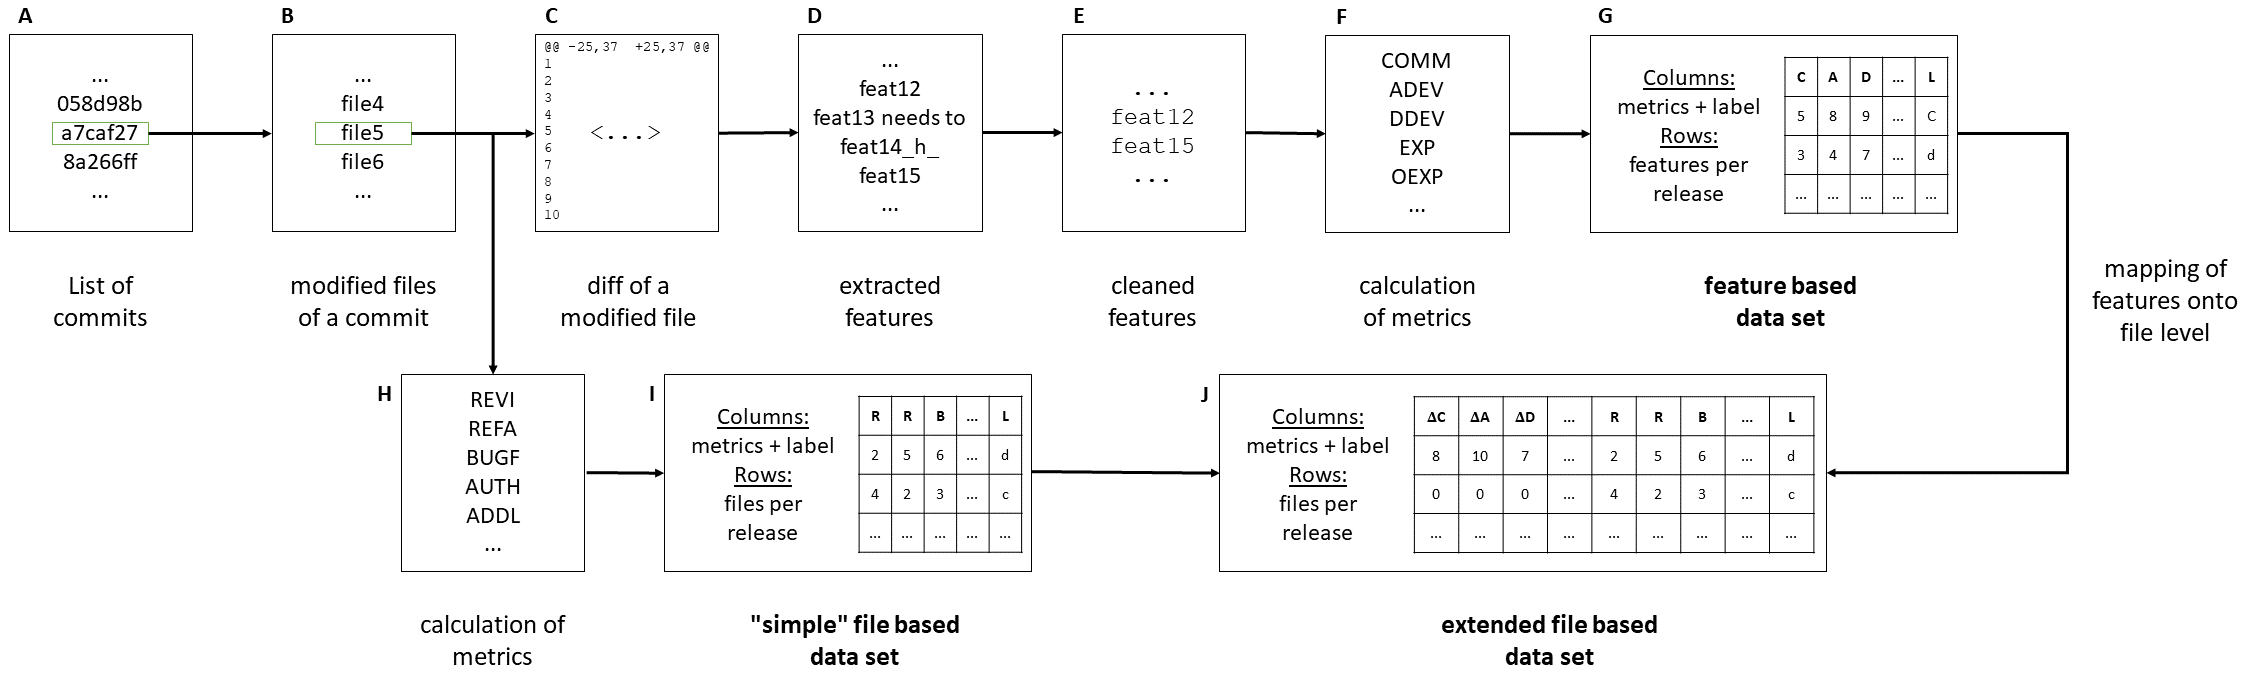
\includegraphics[width=\textwidth]{Dataset}
    \Description{Visualization to distinguish the three data sets.}
    \caption{Visualization to distinguish the three data sets\label{fig:dataset}}
\end{figure*}

The figure shows the ways of creating the feature-based dataset (path A - G) and the file-based data sets according  to \cite{Moser2008}.These are divided into the "simple" file-based dataset (paths A, B, H, I) and the extended file-based dataset (combination of both paths).  The creation of the feature-based dataset has already been explained in detail up to this section. More information about finalizing the datasets will follow as this section progresses.

The creation of the file-based datasets is also based on the raw data of the software project commits obtained with PyDriller and the modified files (A + B) extracted from them. Thus no further processing of the raw data is necessary. They then serve as a basis for the calculation of the 17 metrics (H) according to \cite{Moser2008}. To calculate the time-based metrics \texttt{AAGE} and \texttt{WAGE}, the raw data or the commits listed in the raw data had to be supplemented with their publication date. This was also done with PyDriller. The date of the first commit of a release was chosen as the starting point for calculating the past weeks.

The feature-based and the "simple" file-based dataset (G + I) consist of the calculated feature- (F) and file-related (H) metrics and the labels of the target class. The values of the metrics are calculated for the data of each software project. The resulting tables contain as columns the values of the eleven or 17 metrics and the label (target class) "defective" or "clean" and as rows the features or files aggregated by release.  This means that if a feature or file has been edited multiple times in a release (i.e. it is edited in multiple commits), the average value of the respective metrics within the release is calculated and stored. The procedure for determining the label is performed for each change to a feature or file using the following pattern:

\begin{table}[H]
\centering
\resizebox{\linewidth}{!}{%
\begin{tabular}{>{\hspace{0pt}}p{0.428\linewidth}>{\hspace{0pt}}p{0.046\linewidth}>{\hspace{0pt}}p{0.283\linewidth}>{\hspace{0pt}}p{0.046\linewidth}>{\hspace{0pt}}p{0.187\linewidth}}
bug-introducing       & + & corrective       & = & defective      \\
bug-introducing       & + & not corrective & = & defective      \\
not bug-introducing & + & corrective       & = & clean  \\
not bug-introducing & + & not corrective & = & clean 
\end{tabular}
}
\end{table}

The information on the status of a feature is based on the files on which it is based. If a feature or a file has been edited several times within a release, the label is determined according to the following rules:

\begin{itemize}
\setlength{\itemsep}{-2pt}
\item in the case of features, it is checked whether the feature was marked as "defective" at least once within the release. If this is the case, it is assumed that the feature is broken in the release in question. If this is not the case, the feature is assumed to be clean.
\item in the case of files, the last commit of the files in that release is checked. If the file is marked "clean" there, it is assumed to be error-free. If it is marked as "defective", it is assumed that it is defective in this release.
\end{itemize}

The individual tables created in this way are then concatenated into a common table, resulting in a comprehensive listing of metrics including the associated labels. This list specifies the characteristics a feature or file must have in order to be classified as "defective" or "clean" and serves as a training basis for classifiers for future predictions.

A special feature is the second file-based data set created for the comparison within the evaluation (J). It is based on the "simple" file-based dataset (I) with the metrics from \cite{Moser2008}, but additionally includes the eleven metrics of the feature-based dataset (G) from \autoref{tab:metrics}. For this purpose, the values of the feature-based metrics were mapped or transferred at file level. This means that for each file of a release referenced in the file-based dataset, it was analyzed which features were mentioned in the respective file. From these features, the corresponding metrics of the feature-based dataset were determined and the average value was calculated and entered into the entered dataset. If no features were mentioned in a file, the value 0 is stored for the feature-based metrics. As mentioned at the beginning of this section, this way the feature-based dataset can be compared with a classical file-based dataset, because the conditions for the comparison have been created. A direct comparison between the different datasets is not practical for the reasons mentioned above.

Some supplementary key figures for the datasets are listed in \autoref{tab:dataset-numbers}. The row "unique" indicates how many unique rows are contained in the datasets. The datasets created in the manner described above can now be used to train the classifiers. This process will be explained in the next section.

\begin{table}[ht]
\centering
\caption{Key figures of the data sets}
\label{tab:dataset-numbers}
\resizebox{\linewidth}{!}{%
\begin{tabular}{|l|r|r|r|} 
\hline
                     & \begin{tabular}[c]{@{}r@{}}\textbf{feature-based}\\\textbf{data set}\end{tabular} & \begin{tabular}[c]{@{}r@{}}\textbf{"simple" file-}\\\textbf{based data set}\end{tabular} & \begin{tabular}[c]{@{}r@{}}\textbf{"extended" file-}\\\textbf{based data set}\end{tabular}  \\ 
\hline
\#attributes         & 11 + label                                                                        & 17 + label                                                                               & 28 + label                                                                                  \\ 
\hline
\#data records       & 14.059                                                                            & 76.986                                                                                   & 76.986                                                                                      \\ 
\hline
~ ~thereof defective & 2.735                                                                             & 1.899                                                                                    & 1.899                                                                                       \\ 
\hline
~ ~thereof clean     & 11.324                                                                            & 75.087                                                                                   & 75.087                                                                                      \\ 
\hline
~ ~thereof unique    & 8.447                                                                             & 52.564                                                                                   & 52.783                                                                                      \\
\hline
\end{tabular}
}
\end{table}

\subsection{Selection of Classifiers}

Although programming with the Python programming language was often used to create the data sets, the choice of a machine learning tool was not the library scikit-learn \cite{scikit}, but an independent solution. The WEKA-Workbench\footnote{\href{https://www.cs.waikato.ac.nz/ml/weka/}{https://www.cs.waikato.ac.nz/ml/weka/}} is used as a machine learning tool. This tool proved to be suitable for the underlying task by numerous citations in scientific papers (among others in \cite{Hammouri2018,Queiroz2016,Ratzinger2008}). The WEKA-Workbench (WEKA as acronym for \textbf{W}aikato \textbf{E}nvironment for \textbf{K}nowledge \textbf{A}nalysis) was developed at the University of Waikato in New Zealand and offers a large collection of machine learning algorithms and preprocessing tools for use within a graphical user interface \cite{Weka2016}. There are also interfaces for the Java programming language \cite{Weka2016}. An overview of the selected classification algorithms can be found in \autoref{tab:classifiers}. This also includes the abbreviations of the classifiers that will be used in the following.

\begin{table*}[ht]
\centering
\caption{Selection of classification algorithms}
\label{tab:classifiers}
\begin{tabular}{|l|l|} 
\hline
 \textbf{Algorithm}         & \textbf{Abbreviation}   \\ 
\hline
J48 Decision Trees          & J48                     \\ 
\hline
k-Nearest-Neighbors         & KNN                     \\ 
\hline
Logistic Regression         & LR                      \\ 
\hline
Na\"{\i}ve Bayes                  & NB                      \\ 
\hline
Artificial Neural Networks  & NN                      \\ 
\hline
Random Forest               & RF                      \\ 
\hline
Stochastic Gradient Descent & SGD                     \\ 
\hline
Support Vector Machines     & SVM                     \\
\hline
\end{tabular}
\end{table*}

All classification algorithms presented above are already integrated in the WEKA tool. It receives as input the final data sets in a proprietary file format. The 13 calculated metrics form the attributes, whereas the target class is represented by the labels "defective" and "clean".

The training process of the classifiers took place within the graphical user interface of WEKA. Before the training, the split ratios for the division of the data sets into training data and test data were determined. It was determined individually for each of the software projects used and is based on the number of releases available in each case. However, care was always taken to approximate the commonly used split ratios of 80:20 and 75:25 as well as 70:30. The training data ranges from 67\% to 80\% of the data records of the data sets. The earlier releases were assigned to the training data. The training data contains the data records of the later releases. An overview of the division into training and test data per software project is shown in \autoref{fig:splits}. The resulting split ratios for the entire data sets are: 69:31 (feature-based data set) and 71:29 ("simple" and extended file-based data set).

\begin{figure*}[ht]
  \centering
  \subfloat[][Blender\\split ratio: 73:27]{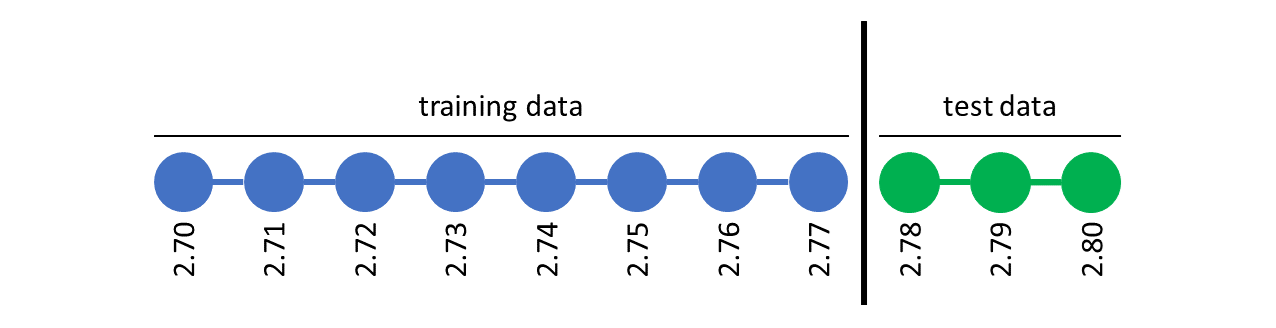
\includegraphics[width=0.5\linewidth]{release_blender}}
  \subfloat[][Busybox\\split ratio: 71:29]{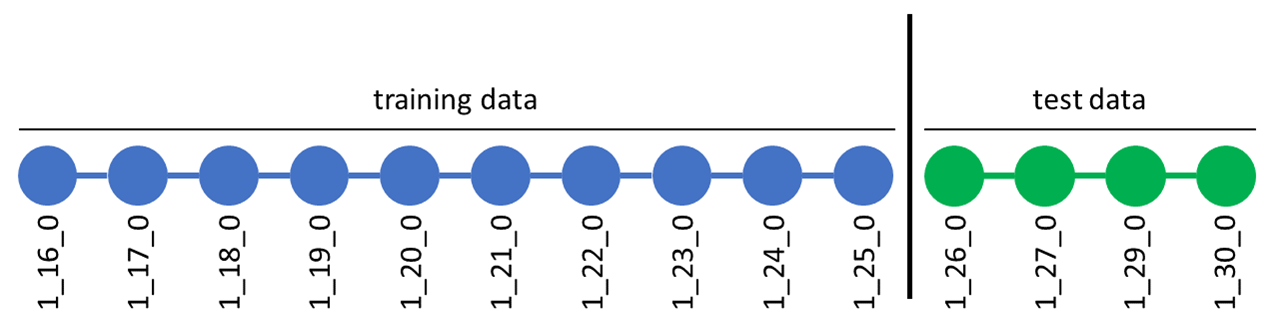
\includegraphics[width=0.5\linewidth]{release_busybox}}
  \qquad
  \subfloat[][Emacs\\split ratio: 71:29]{
\includegraphics[width=0.5\linewidth]{release_emacs}}
  \subfloat[][GIMP\\split ratio: 71:29]{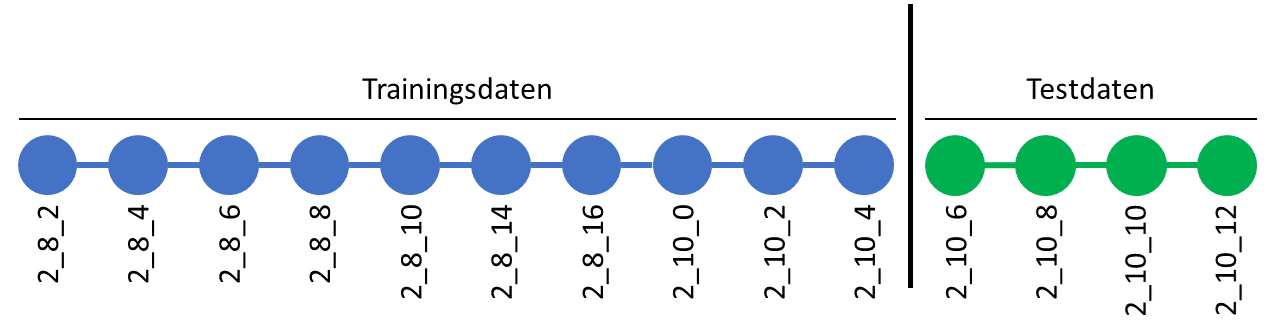
\includegraphics[width=0.5\linewidth]{release_gimp}}
  \qquad
  \subfloat[][Gnumeric\\split ratio: 75:25]{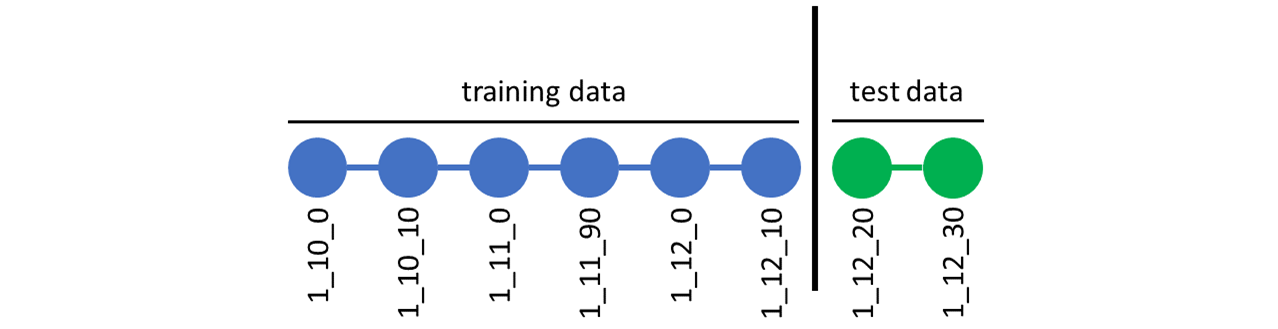
\includegraphics[width=0.5\linewidth]{release_gnumeric}}  
  \subfloat[][gnuplot\\split ratio: 80:20]{
\includegraphics[width=0.5\linewidth]{release_gnuplot}}
  \qquad
  \subfloat[][Irssi\\split ratio: 71:29]{
\includegraphics[width=0.5\linewidth]{release_irssi}}
  \subfloat[][libxml2\\split ratio: 80:20]{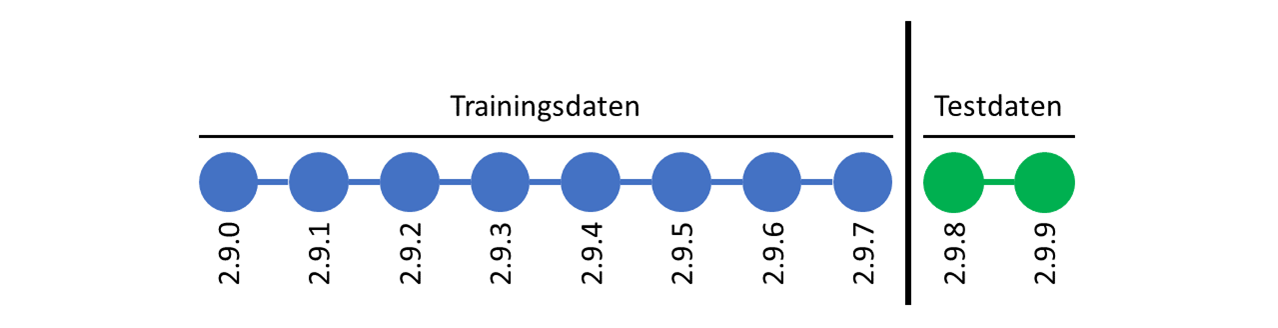
\includegraphics[width=0.5\linewidth]{release_libxml2}}
  \qquad
  \subfloat[][lighttpd\\split ratio: 67:33]{
\includegraphics[width=0.5\linewidth]{release_lighttpd}}
  \subfloat[][MPSolve\\split ratio: 75:25]{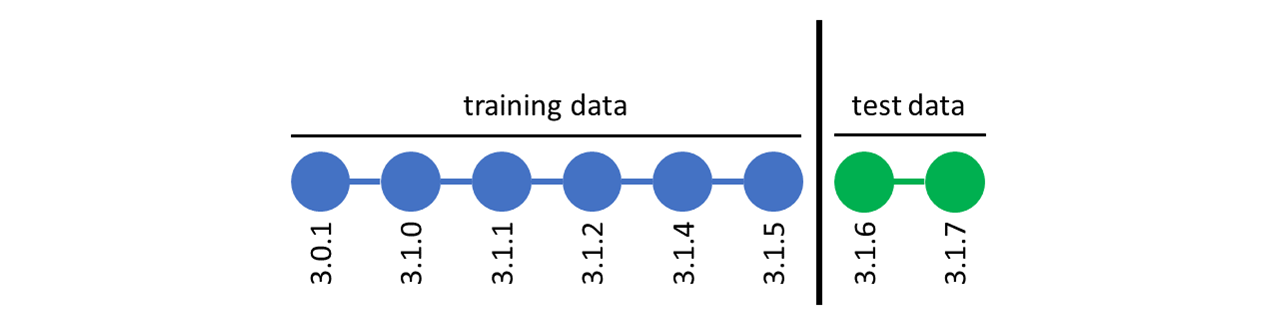
\includegraphics[width=0.5\linewidth]{release_mpsolve}}
  \qquad
  \subfloat[][Parrot\\split ratio: 71:29]{
\includegraphics[width=0.5\linewidth]{release_parrot}}
  \subfloat[][Vim\\split ratio: 71:29]{
\includegraphics[width=0.5\linewidth]{release_vim}}
  \Description{Overview of the division into training and test data.}
  \caption{Overview of the division into training and test data\label{fig:splits}}
\end{figure*}

The training of the classifiers in WEKA was carried out for each classification algorithm with the respective standard settings. Only for the algorithms NN and RF further configurations were made. For the RF-algorithm a number of instances of 200 was defined. This means that 200 decision trees are processed simultaneously in parallel. For the NN algorithm a hidden layer structure of \texttt{(13,13,13} was chosen. This means that the artificial neural network has three hidden layer layers of 13 hidden layer neurons each. This allows them to process the large number of attributes more efficiently. Furthermore, no validation data was generated, since it is not intended to perform attribute selection or to adjust further classifier settings.

An analysis of the training process also showed that the file-based data sets are highly unbalanced with regard to the target class. With a value of about 97\% there are far more entries that are assigned to the label "clean". Balancedness, i.e. a balanced ratio (50:50 is not mandatory in the binary case) within the target classes, is however a prerequisite for the correct training of most classifiers. Ignoring this problem can lead to a misleading accuracy (hit accuracy of the classifier), because most data sets are correctly assigned to the overrepresented class. To solve this problem, the SMOTE algorithm was applied to the file-based datasets \cite{Chawla2002}. The algorithm, whose acronym stands for \textbf{S}ynthetic \textbf{M}inority \textbf{O}ver-sampling \textbf{Te}chnique, performs an oversampling of the underrepresented class \cite{Chawla2002}. Using next-neighbor calculations based on the Euclidean distance between the attribute values of each dataset's datasets, new synthetic datasets are added (oversampling) so that the number of datasets of the relevant class increases \cite{Chawla2002}. In this case, the percentage of synthetic records generated is 2000, so for each existing record of the underrepresented class, 20 additional synthetic records are generated. Thus, the percentage of records labeled "defective" was increased to about 41\%. At the same time the number of records grew by about 60\%. The algorithm was only applied to the training data \cite{Chawla2002} . An application to the test data is not foreseen, so that the "ground truth" is not distorted or falsified. As a result, the metrics of the file-based datasets also changed. These are shown in \autoref{tab:dataset-numbers-new}.

\begin{table*}[ht]
\centering
\caption{Key figures of the data sets}
\label{tab:dataset-numbers-new}
\begin{tabular}{|l|r|r|r|r|} 
\hline
\multirow{2}{*}{}    & \multicolumn{2}{c|}{\textbf{"simple" data set}} & \multicolumn{2}{c|}{\textbf{extended data set}}  \\ 
\cline{2-5}
                     & \textbf{before} & \textbf{after}                & \textbf{before} & \textbf{after}                 \\ 
\hline
\#attributes         & 17 + label      & 17 + label                    & 28 + label      & 28 + label                     \\ 
\hline
\#data records       & 76.986          & 111.706                       & 76.986          & 112.706                        \\ 
\hline
~ ~thereof defective & 1.899           & 37.619                        & 1.899           & 37.619                         \\ 
\hline
~ ~thereof clean     & 75.087          & 75.087                        & 75.087          & 75.087                         \\ 
\hline
~ ~thereof unique    & 52.564          & 86.155                        & 52.783          & 86.381                         \\ 
\hline
overall split ratio  & 71:29           & 81:19                         & 71:29           & 81:19                          \\
\hline
\end{tabular}
\end{table*}

The results obtained using the test data, which reflect the performance of the individual classifiers, are presented in the following chapter as part of the evaluation.

% !TEX root = ../thesis.tex

\chapter{Evaluation}
\label{evaluation}

Dieses Kapitel dient der Evaluation der im vorangegangenen Kapitel erläuterten Klassifikatoren, die auf den drei in \hyperref[dataset-creation]{Kapitel 3} vorgestellten Datensets basieren und auf der Grundlage der Daten von 12 featurebasierten Softwareprojekten aufgebaut wurden. Bei diesen handelt es sich wiederum um das feautrebasierte Datenset sowie das \glqq einfache\grqq{} und das erweiterte dateibasierte Datenset, welches zusätzlich die Metriken des featurebasierten Datensets, auf Dateiebene gemapped, enthält. Die Datensets bestehen jeweils aus den Attributen sowie dem Label als Spalten und in den Zeilen die zugehörigen Werte für jedes Feature beziehungsweise jede Datei aggregiert nach Release. Die Evaluation geschieht durch verschiedene Evaluationsmetriken, welche in diesem Kapitel vorgestellt werden und auf Werten von sogenannten Konfusionsmatrizen und ROC-Kurven basieren. Erweitert wird dieser Teil der Evaluation mit dem Vergleich zwischen dem \glqq einfachen\grqq{} und erweiterten dateibasierten Datenset zur Messung der Einflüsse der featurebasierten Metriken auf die Performanz der Vorhersagen. Zudem umfasst dieses Kapitel eine Erläuterung von Herausforderungen und Limitationen, die im Laufe der Bearbeitung der Arbeit festgestellt wurden. Es werden somit die Arbeitsschritte erläutert, welche durchgeführt wurden, um das dritte Forschungsziel \glqq Evaluation und Gegenüberstellung der Klassifikatoren sowie Vergleich zu einer klassischen Vorhersagetechnik, die keine Features nutzt\grqq{} abzuschließen. Darüber hinaus werden die folgenden zugehörigen Forschungsfragen beantwortet:
\vspace{-\topsep}
\begin{itemize}
\setlength{\itemsep}{-2pt}
 \item RQ3a: Welches Vorgehen bietet sich zum internen Vergleich der Klassifikatoren an? (\hyperref[eval-metrics]{Abschnitt 5.1})
 \item RQ3b: Welche Ergebnisse können bei der Vorhersage von fehlerhaften oder fehlerfreien Features erzielt werden? (\hyperref[feat-results]{Abschnitt 5.2.1})
 \item RQ3d: Wie beeinflusst die Verwendung von featurebasierten Metriken die dateibasierte Fehlervorhersage? (\hyperref[classic-eval]{Abschnitt 5.2.2})
\end{itemize} 
\smallskip
\hrule

\section{Evaluationsmetriken}
\label{eval-metrics}

Die zum Vergleich der Klassifikatoren erhobenen Evaluationsmetriken entstammen dem Themengebiet des Information Retrieval und gelten als Standardmesswerte für ihren Einsatzzweck \cite{Sammut2017}. Die meisten dieser Metriken lassen sich anhand von Werten einer sogenannten Konfusionsmatrix berechnen und messen allesamt die Performanz der Vorhersagen von Klassifikatoren unter verschiedenen Betrachtungsweisen. Im Falle einer binären Klassifikation,  wie sie auch dieser Arbeit zugrunde lag, besteht diese Matrix aus vier Gruppen, deren Werte angeben, ob der jeweilige Klassifikator ein Objekt korrekt oder falsch einer der beiden Zielklassen zuordnen konnte \cite{Sammut2017}. Im Zusammenhang mit solchen Matrizen werden die beiden Zielklassen \glqq positiv\grqq{} und \glqq negativ\grqq{} genannt. Für diese Arbeit werden die positive Klasse dem Label \glqq defekt\grqq und die negative Klasse dem Label \glqq fehlerfrei\grqq{} zugeordnet. Die Form einer allgemeinen Konfusionsmatrix ist in \autoref{fig:confu} dargestellt.

\begin{figure}[H]
    \centering
    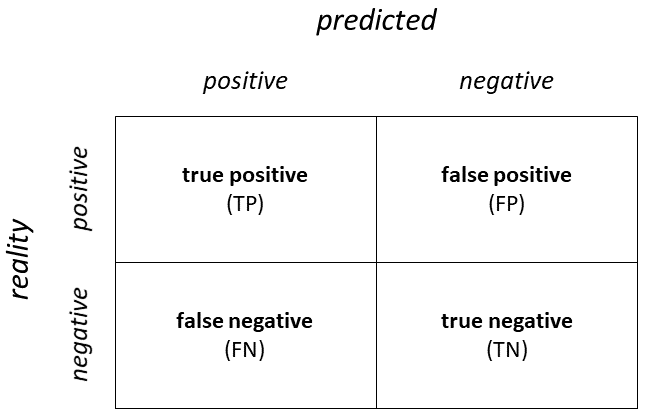
\includegraphics[width=0.7\textwidth]{images/Confusion}
    \caption{allgemeine Konfusionsmatrix\label{fig:confu}}
\end{figure}

Das zum Training der Klassifikatoren verwendete Werkzeug WEKA besitzt die Option, Konfusionsmatrizen zu den durchgeführten Tests der Klassifikatoren auszugeben. Anhand der Werte der Zuordnungen zu den zuvor genannten Gruppen wurden die folgenden Evaluationsmetriken berechnet: 

\begin{itemize}
\item Treffergenauigkeit (Accuracy)
\\Dieser Wert misst die Treffergenauigkeit der Vorhersagen des Klassifikators und gibt an, inwieweit dessen Vorhersagen mit der modellierten Realität übereinstimmen \cite{Sammut2017}. Die Formel zur Berechnung der Accuracy lautet:
\\\[\text{Accuracy} = \frac{TP+TN}{TP+TN+FP+FN}\]
Das Ergebnis der Berechnung ist ein prozentualer Wert. $100\%$ stellen damit die bestmögliche Accuracy dar. In diesem Fall werden alle Vorhersagen korrekt, mit der Realität übereinstimmend, getroffen.
\item Echt-Positiv-Rate / Trefferquote (TP-Rate / Recall)
\\Dieser Wert gibt den Anteil der korrekt als positiv gewerteten Vorhersagen sämtlicher als positiv gewerteter Vorhersagen an \cite{Alpaydin2010}. Die Formel zur Berechnung der TP-Rate bzw. des Recalls lautet:
\\\[\text{TP-Rate} = \frac{TP}{TP+FN}\]
Das Ergebnis der Berechnung ist ein prozentualer Wert. $100\%$ stellen damit die bestmögliche TP-Rate bzw. den bestmöglichen Recall dar. In diesem Fall werden alle positiven Vorhersagen korrekt getroffen. Beide Begriffe werden parallel für die Berechnung der gezeigten Formel verwendet.
\item Positiver Vorhersagewert (Precision)
\\ Dieser Wert gibt die Anzahl der positiven Vorhersagen an, die auch tatsächlich zur positiven Klasse gehören \cite{Sammut2017}. Die Formel zur Bestimmung der Precision lautet:
\\\[\text{Precision} = \frac{TP}{TP+FP}\]
Das Ergebnis der Berechnung ist ein prozentualer Wert. $100\%$ stellen damit die bestmögliche Precision dar. In diesem Fall werden nur korrekte positive Vorhersagen getroffen.
\item F-Maß (F-Score)
\\ Dieser Wert berechnet das harmonische Mittel der Werte Precision und Recall und liegt somit zwischen diesen beiden Werten, jedoch näher am kleineren Wert \cite{Sammut2017}. Die Formel zur Berechnung des F-Scores lautet:
\\\[\text{F-Score} = \frac{2TP}{2TP+FP+FN}\]
Das Ergebnis der Berechnung ist ein prozentualer Wert. $100\%$ stellen damit den bestmöglichen F-Score dar. In diesem Fall wurden alle positiven Vorhersagen korrekt getroffen.
\end{itemize}

\label{roc-def}
Um eine weiteren Messwert für die Vorhersageperformanz und die Qualität der Vorhersagen zu erhalten, wurden die sogenannten ROC-Kurven (englisch: ROC curves, ROC = Receiver Operating characteristic, deutsch: Betriebsverhalten des Empfängers) der einzelnen Klassifikatoren ermittelt. Diese besitzen den Vorteil, dass sie einfach und verständlich die Performanz der Klassifikatoren abbilden und die Qualität der Vorhersagen \glqq sichtbar\grqq{} machen. Dazu genügt es lediglich, Standardverläufe der Kurven zu kennen, die im weiteren Verlauf exemplarisch anhand eines Beispiels dargestellt werden.
Bei den ROC-Kurven handelt es sich um Wahrscheinlichkeitsverteilungen, die das Verhältnis zwischen der TP-Rate (y-Achse) und der Falsch-Positiv-Rate (x-Achse) beschreiben \cite{Sammut2017,Narkhede2018}. Die Falsch-Positiv-Rate (FP-Rate) gibt dabei den Anteil der fälschlicherweise als positiv gewerteten Vorhersagen an \cite{Alpaydin2010}. Sie wird mittels folgender Formel berechnet:
\\\[\text{FP-Rate} = \frac{FP}{FP+TN}\]

Wie bei allen Metriken ist das Ergebnis der FP-Rate ein prozentualer Wert. Im Gegensatz zu den vorherigen Metriken, sollte dieses Ergebnis bestenfalls möglichst gering ausfallen. Sowohl die TP-Rate als auch die FP-Rate geben nur singuläre Werte an, aus welchen sich keine Graphen herleiten lassen. Jeder Klassifikator errechnet jedoch im Rahmen der Vorhersage eines Datenpunktes Wahrscheinlichkeiten, die die Zugehörigkeit zu den Werten der Zielklasse darstellen \cite{KNIMETV2019}. In der Regel wird ein Datenpunkt der positiven Klasse zugeordnet, wenn die Wahrscheinlichkeit einen Schwellenwert von $0,5$ übersteigt - Datenpunkte, die diesen Schwellenwert unterschreiten werden hingegen der negativen Klasse zugeordnet \cite{KNIMETV2019}. Wird der Schwellenwert erhöht, so werden weniger Datenpunkte der positiven Klasse zugeordnet, wohingegen im Falle einer Absenkung des Schwellenwertes mehr Datenpunkte der positiven Klasse zugeordnet werden \cite{KNIMETV2019}. Für die Erstellung der ROC-Kurven werden somit die Werte der TP-Rate und der FP-Rate unter der Berücksichtigung der Schwellenwerte im Bereich von $0,0$ bis $1,0$ gegenübergestellt.

Eine weitere Metrik, die in Verbindung mit der ROC-Kurve auftritt, ist der ROC-Bereich (ROC area). Dieser Wert, der anhand der ROC-Kurve berechnet wird und auch AUC-Bereich (AUC = Area Under Curve, Bereich unter der Kurve) genannt wird, gibt an, inwieweit ein Klassifikator in der Lage ist, zwischen den Werten der Zielklassen zu unterscheiden \cite{Narkhede2018}. Je höher dieser Wert ist ($1,0$ ist das Maximum), desto besser trifft der Klassifikator korrekte Vorhersagen \cite{Narkhede2018}. Er spiegelt somit die Qualität der Vorhersagen wider.

Am Beispiel des Schwellenwertes $0,5$ wird nun die Interpretation der ROC-Kurve und des ROC-Bereiches vorgenommen. Unterstützt wird dies durch grafische Beispiele, die in \autoref{fig:curves} gezeigt werden. Der Idealfall ist in (a) und (b) dargestellt. Die Wahrscheinlichkeitskurven der Zielklasse (a) weisen keine Überlappung auf. Die Werte der Zielklasse sind somit allesamt korrekt zugeordnet worden, sodass der Klassifikator korrekt zwischen diesen unterscheiden kann. Die diesem Fall entsprechende ROC-Kurve ist in (b) dargestellt. Der ROC-Bereich beträgt in diesem Fall $1,0$. Ein \glqq Normalfall\grqq{} ist in (c) und (d) dargestellt. Es ist in (c) zu erkennen, dass die Wahrscheinlichkeitskurven überlappen, sodass falsche Zuordnungen getroffen werden. Die entsprechende ROC-Kurve ist in (d) dargestellt. Der entsprechende ROC-Bereich beträgt im hier gezeigten Fall $0,7$. Dies bedeutet, dass $70\%$ der Zuordnungen richtig getroffen werden. Die Werte können verbessert werden, wenn der Schwellenwert verändert wird. Der \glqq Worst Case\grqq{} der bei der Performanzmessung mittels ROC-Kurven auftreten kann, ist in (e) und (f) dargestellt. In (e) ist zu erkennen, dass die Wahrscheinlichkeitskurven identisch sind. Es findet somit eine willkürliche Zuordnung statt. Die zugehörige ROC-Kruve (f) entspricht einer Winkelhalbierenden und der ROC-Bereich beträgt $0,5$. Ein weiterer Fehlerfall ist in (g) und (h) dargestellt. Die Wahrscheinlichkeitskurven in (g) zeigen, dass die Zuordnungen gegenteilig erfolgen und somit jeweils fälschlicherweise dem anderen Wert der Zielklasse zugeordnet werden. Der entsprechende ROC-Bereich beträgt $0$, da, wie in (h) zu sehen ist, keine Fläche unter der Kurve vorhanden ist.

\begin{figure}[p]
  \centering
  \subfloat[][Idealfall]{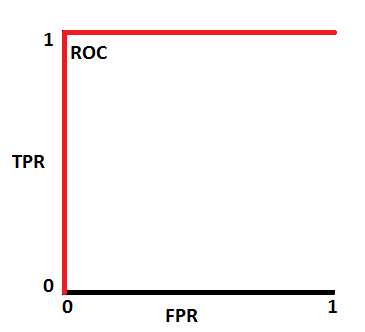
\includegraphics[width=0.5\linewidth]{images/roc_ideal_curve}}
  \subfloat[][Idealfall]{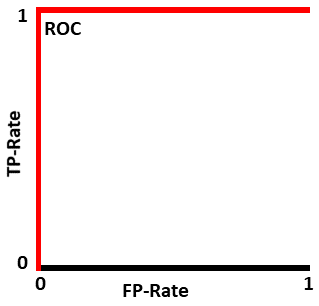
\includegraphics[width=0.25\linewidth]{images/roc_ideal}}
  \qquad
  \subfloat[][\glqq Normalfall\grqq]{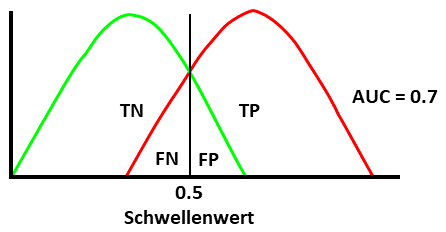
\includegraphics[width=0.5\linewidth]{images/roc_normal_curve}}
  \subfloat[][\glqq Normalfall\grqq]{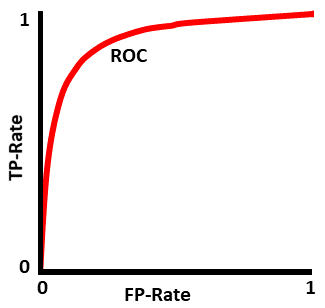
\includegraphics[width=0.25\linewidth]{images/roc_normal}}
  \qquad
  \subfloat[][\glqq Worst Case\grqq]{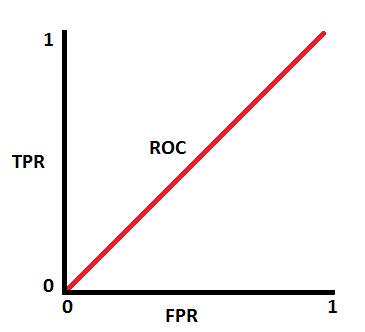
\includegraphics[width=0.3\linewidth]{images/roc_worst_curve}}
  \subfloat[][\glqq Worst Case\grqq]{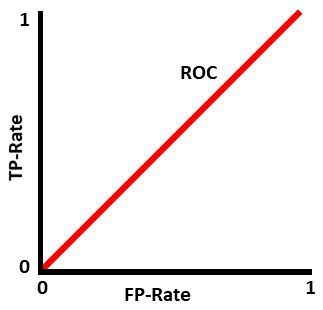
\includegraphics[width=0.25\linewidth]{images/roc_worst}}
  \qquad
  \subfloat[][Fehlerfall]{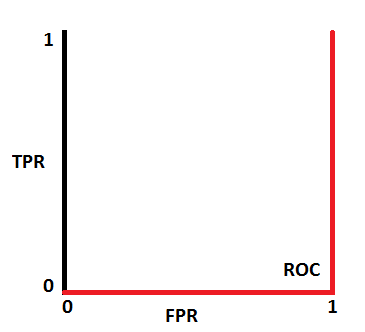
\includegraphics[width=0.5\linewidth]{images/roc_neg_curve}}
  \subfloat[][Fehlerfall]{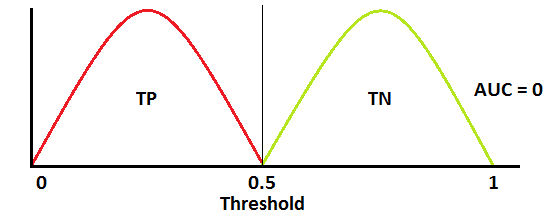
\includegraphics[width=0.25\linewidth]{images/roc_neg}}
  \caption{Beispiel zur Interpretation der ROC-Kurve und des ROC-Bereiches (TPR = TP-Rate, FPR = FP-Rate, Threshold = Schwellenwert) \cite{Narkhede2018}
\label{fig:curves}}
\end{figure}

Alle vorgestellten Metriken werden automatisiert von WEKA berechnet. Ferner besitzt das Werkzeug die Fähigkeit, ROC-Kurven mit den entsprechenden ROC-Werten auszugeben. Die im Rahmen der Evaluation der Klassifikatoren ermittelten Werte der Metriken sowie die ROC-Kurven und Werte der ROC-Bereiche werden im folgenden Abschnitt aufgeführt sowie verglichen und interpretiert.

\fbox{\parbox{\linewidth}{RQ3a: WELCHES VORGEHEN BIETET SICH ZUM INTERNEN VERGLEICH DER KLASSIFIKATOREN AN?\medskip\\
Das Vorgehen zum internen Vergleich der Klassifikatoren umfasst die Betrachtung von Evaluationsmetriken, welche auf Basis der Ergebnisse des Tests der Klassifikatoren errechnet werden und die Performanz der Vorhersagen auf verschiedene Weisen messen. Für den Vergleich werden klassische Evaluationsmetriken verwendet, welche auf Basis von Konfusionsmatrizen berechnet werden. Die betrachteten Metriken lauten: Accuracy, TP-Rate / Recall, Precision und F-Score. Ebenfalls hinzugezogen werden die jeweiligen ROC-Kurven der Klassifikatoren inklusive der ROC-Bereiche. Diese Metriken stellen einen Standard für die Messung der Performanz der Vorhersagen von Klassifikatoren dar.}}

\section{Ergebnisse und Diskussion}
\label{results}

Dieser Abschnitt umfasst die Ergebnisse und vergleichenden Diskussionen zu den Tests der Klassifikatoren der drei Datensets, aufgeteilt in einen Unterabschnitt für das featurebasierte Datenset und einen Unterabschnitt für die dateibasierten Datensets. Darüber hinaus sind die jeweiligen Unterabschnitte wie folgt aufgeteilt: Konfusionsmatrizen, Accuracies, weitere Evaluationsmetriken, ROC-Kurven und ROC-Bereiche sowie Zusammenfassung.

\subsection{Ergebnisse und Vergleich der featureabsierten Klassifikatoren}
\label{feat-results}

Die Präsentation der Ergebnisse beginnt mit denen der Klassifikatoren des featurebasierten Datensets. Darüber hinaus wird die folgende Forschungsfrage im Fließtext sowie zusammengefasst am Ende des Abschnitts beantwortet:
\vspace{-\topsep}
\begin{itemize}
\setlength{\itemsep}{-2pt}
 \item RQ3b: Welche Ergebnisse können bei der Vorhersage von fehlerhaften oder fehlerfreien Features erzielt werden?
\end{itemize}

Auf Basis der Betrachtung der Ergebnisse der Evaluationsmetriken kann die Performanz hinsichtlich der Vorhersagen von fehlerhaften oder fehlerfreien Features gemessen und interpretiert werden.  

\paragraph{Konfusionsmatrizen}
Die Konfusionsmatrizen dienen als Basis der Ergebnisse der Evaluation der Klassifikatoren anhand der zuvor vorgestellten Metriken. Die Matrizen des featurebasierten Datensets sind in \autoref{tab:mat-feat} aufgeführt. Dabei bilden die Spalten die von den Klassifikatoren vorhergesagten Label ab. Die Zeilen bilden wiederum die \glqq ground truth\grqq{}, also die im Rahmen der Erstellung der Datensets ermittelte Realität, ab. Außerdem werden die ermittelten Werte der jeweiligen Klassen in den Spalten \glqq total\grqq zusammengezählt. Da für jeden Klassifikator dasselbe Testset gewählt wurde, sind die Werte der \glqq total\grqq-Spalte identisch. Die für die Klassifikatoren verwendeten Abkürzungen können \autoref{tab:classifiers} entnommen werden.

\begin{table}[h!t]
\centering
\caption{Konfusionsmatrizen des featurebasierten Datensets}
\label{tab:mat-feat}
\resizebox{\linewidth}{!}{%
\begin{tabular}{|>{\hspace{0pt}}p{0.119\linewidth}>{\hspace{0pt}}p{0.362\linewidth}|>{\RaggedLeft\hspace{0pt}}p{0.156\linewidth}>{\RaggedLeft\hspace{0pt}}p{0.214\linewidth}>{\RaggedLeft\hspace{0pt}}p{0.139\linewidth}|} 
\cline{2-5}
\multicolumn{1}{>{\Centering\hspace{0pt}}p{0.119\linewidth}|}{} & \textbf{Ermittelt -\textgreater{}} & \textbf{defekt}  & \textbf{fehlerfrei}  & \textbf{total}  \\ 
\hline
\multirow{3}{0.119\linewidth}{\hspace{0pt}J48}                  & Realität defekt                    & $446$              & $320$                  & $766$             \\
                                                                & Realität fehlerfrei                & $483$              & $3.142$                & $3.625$           \\
                                                                & total                              & $929$              & $3.462$                & $4.391$           \\ 
\hline
\multirow{3}{0.119\linewidth}{\hspace{0pt}KNN}                  & Realität defekt                    & $371$              & $395$                  & $766$             \\
                                                                & Realität fehlerfrei                & $569$              & $3.056$                & $3.625$           \\
                                                                & total                              & $940$              & $3.451$                & $4.391$           \\ 
\hline
\multirow{3}{0.119\linewidth}{\hspace{0pt}LR}                   & Realität defekt                    & $309$              & $457$                  & $766$             \\
                                                                & Realität fehlerfrei                & $1.020$            & $2.605$                & $3.625$           \\
                                                                & total                              & $1.329$            & $3.061$                & $4.391$           \\ 
\hline
\multirow{3}{0.119\linewidth}{\hspace{0pt}NB}                   & Realität defekt                    & $322$              & $444$                  & $766$             \\
                                                                & Realität fehlerfrei                & $265$              & $3.360$                & $3.625$           \\
                                                                & total                              & $587$              & $3.804$                & $4.391$           \\ 
\hline
\multirow{3}{0.119\linewidth}{\hspace{0pt}NN}                   & Realität defekt                    & $327$              & $439$                  & $766$             \\
                                                                & Realität fehlerfrei                & $1.019$            & $2.60$6                & $3.625$           \\
                                                                & total                              & $1.346$            & $3.045$                & $4.391$           \\ 
\hline
\multirow{3}{0.119\linewidth}{\hspace{0pt}RF}                   & Realität defekt                    & $504$              & $262$                  & $766$             \\
                                                                & Realität fehlerfrei                & $450$              & $3.175$                & $3.625$           \\
                                                                & total                              & $954$              & $3.437$                & $4.391$           \\ 
\hline
\multirow{3}{0.119\linewidth}{\hspace{0pt}SGD}                  & Realität defekt                    & $251$              & $515$                  & $766$             \\
                                                                & Realität fehlerfrei                & $938$              & $2.687$                & $3.625$           \\
                                                                & total                              & $1.189$            & $3.202$                & $4.391$           \\ 
\hline
\multirow{3}{0.119\linewidth}{\hspace{0pt}SVM}                  & Realität defekt                    & $176$              & $590$                  & $766$             \\
                                                                & Realität fehlerfrei                & $899$              & $2.726$                & $3.625$           \\
                                                                & total                              & $1.075$            & $3.316$                & $4.391$           \\
\hline
\end{tabular}
}
\end{table}

\paragraph{Accuracies}
Die erste Metrik die verglichen wird ist die Accuracy. Dargestellt werden die Ergebnisse zum besseren Vergleich als Balkendiagramme. Das Diagramm des feturebasierten Datensets ist in \autoref{fig:final-feat} dargestellt. Die konkreten Zahlenwerte können im \hyperref[appendix2]{Anhang} eingesehen werden.

\begin{figure}[h!t]
    \centering
    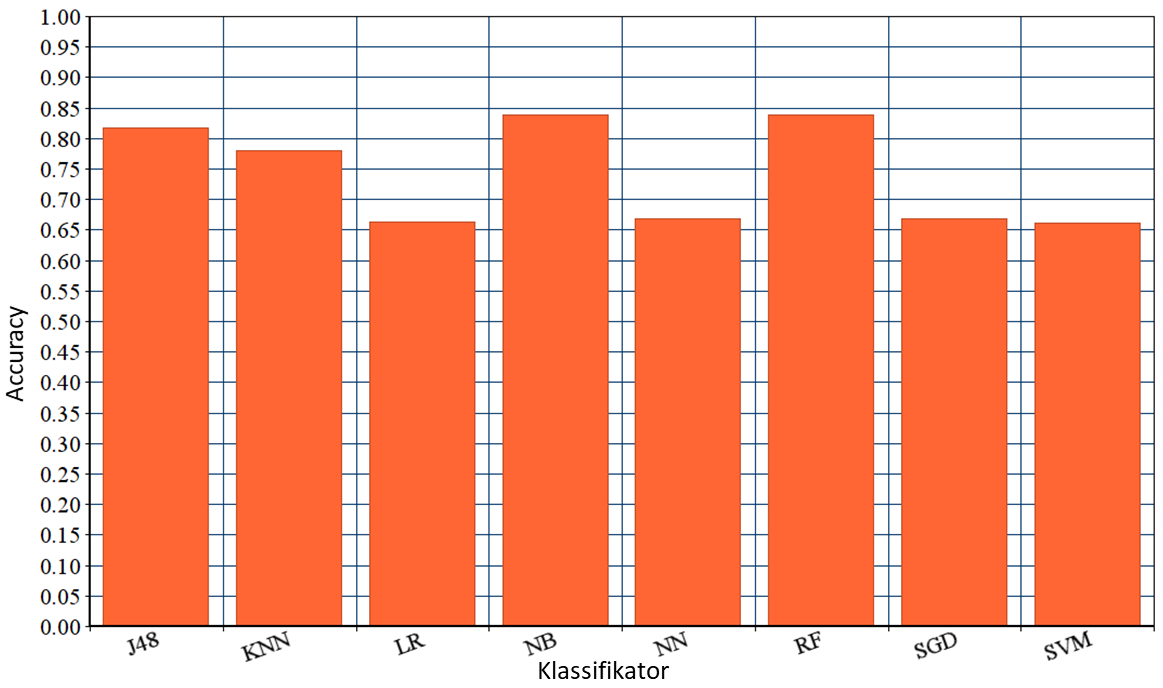
\includegraphics[width=\textwidth]{images/final_feat}
    \caption{Vergleich der Accuracies des featurebasierten Datensets\label{fig:final-feat}}
\end{figure}

Die Ergebnisse zeigen, dass die Accuracies der Klassifikatoren zwischen $66\%$ und $84\%$ liegen. Die höchsten Werte erreichten die Klassifikatoren NB und RF mit einer Treffergenauigkeit von jeweils $84\%$. Mit einem Wert von $82\%$ erreichte auch der J48-Klassifikator eine überdurchschnittlich hohe Performanz. Darauf folgt der KNN-Klassifikator mit $78\%$. Mit Werten von $66\%$ beziehungsweise $67\%$ schnitten die Klassifikatoren LR, NN, SGD und SVM am schlechtesten ab. Sie ermittelten somit in über $30\%$ der Vorhersagen ein falsches Ergebnis. Auffällig an diesen Ergebnissen ist die hohe Performanz beider Entscheidungsbaum-basierter Klassifikatoren J48 und RF. Sie scheinen somit die Eingabemenge am besten verarbeiten zu können, um Rückschlüsse auf die neuen Daten in Form der Testdaten ziehen zu können.

\paragraph{TP-Rate / Recall, FP-Rate, Precision, F-Score}
Dieser Abschnitt stellt die Ergebnisse der weiteren Evaluationsmetriken TP-Rate / Recall, FP-Rate, Precision und F-Score vor. Diese können in \autoref{tab:met-results-feat} für das featurebasierte Datenset eingesehen werden. Aufgeteilt werden die Ergebnisse nach den Werten der Zielklasse, \glqq defekt\grqq{} und \glqq fehlerfrei\grqq. Zudem wird der Mittelwert der Ergebnisse beider Werte der Zielklasse angegeben. Er zeigt die Performanz aggregiert für beide Werte an und liegt im Idealfall bei 1,00. Die vollständigen Tabellen der Ergebnisse der Evaluation, inklusive einer weiteren Metrik, können im \hyperref[appendix3]{Anhang} gefunden werden.

\begin{table}[h!t]
\centering
\caption{Ergebnisse der Evaluationsmetriken des featurebasierten Datensets}
\label{tab:met-results-feat}
\resizebox{\linewidth}{!}{%
\begin{tabular}{|>{\hspace{0pt}}p{0.12\linewidth}>{\hspace{0pt}}p{0.349\linewidth}|>{\RaggedLeft\hspace{0pt}}p{0.156\linewidth}>{\RaggedLeft\hspace{0pt}}p{0.214\linewidth}>{\RaggedLeft\hspace{0pt}}p{0.141\linewidth}|} 
\cline{3-5}
\multicolumn{1}{>{\hspace{0pt}}p{0.12\linewidth}}{} &                  & \textbf{defekt}  & \textbf{fehlerfrei}  & \textbf{Mittel}   \\ 
\hline
\multirow{4}{0.12\linewidth}{\hspace{0pt}J48}       & TP-Rate / Recall & $0,58$             & $0,87$                 & $0,73$              \\
                                                    & FP-Rate          & $0,13$             & $0,42$                 & $0,28$              \\
                                                    & Precision        & $0,48$             & $0,91$                 & $0,70$              \\
                                                    & F-Score          & $0,53$             & $0,89$                 & $0,71$              \\ 
\hline
\multirow{4}{0.12\linewidth}{\hspace{0pt}KNN}       & TP-Rate / Recall & $0,48$             & $0,86$                 & $0,67$              \\
                                                    & FP-Rate          & $0,16$             & $0,52$                 & $0,68$              \\
                                                    & Precision        & $0,40$             & $0,89$                 & $0,65$              \\
                                                    & F-Score          & $0,44$             & $0,86$                 & $0,66$              \\ 
\hline
\multirow{4}{0.12\linewidth}{\hspace{0pt}LR}        & TP-Rate / Recall & $0,40$             & $0,72$                 & $0,56$              \\
                                                    & FP-Rate          & $0,28$             & $0,60$                 & $0,44$              \\
                                                    & Precision        & $0,23$             & $0,85$                 & $0,54$              \\
                                                    & F-Score          & $0,30$             & $0,78$                 & $0,54$              \\ 
\hline
\multirow{4}{0.12\linewidth}{\hspace{0pt}NB}        & TP-Rate / Recall & $0,42$             & $0,93$                 & $0,68$              \\
                                                    & FP-Rate          & $0,07$             & $0,58$                 & $0,33$              \\
                                                    & Precision        & $0,55$             & $0,88$                 & $0,72$              \\
                                                    & F-Score          & 0,48             & $0,91$                 & $0,70$              \\ 
\hline
\multirow{4}{0.12\linewidth}{\hspace{0pt}NN}        & TP-Rate / Recall & $0,43$             & $0,72$                 & $0,58$              \\
                                                    & FP-Rate          & $0,28$             & $0,57$                 & $0,43$              \\
                                                    & Precision        & $0,24$             & $0,86$                 & $0,55$              \\
                                                    & F-Score          & $0,31$             & $0,78$                 & $0,55$              \\ 
\hline
\multirow{4}{0.12\linewidth}{\hspace{0pt}RF}        & TP-Rate / Recall & $0,66$             & $0,8$8                 & $0,77$              \\
                                                    & FP-Rate          & $0,12$             & $0,34$                 & $0,23$              \\
                                                    & Precision        & $0,53$             & $0,92$                 & $0,73$              \\
                                                    & F-Score          & $0,59$             & $0,90$                 & $0,75$              \\ 
\hline
\multirow{4}{0.12\linewidth}{\hspace{0pt}SGD}       & TP-Rate / Recall & $0,34$             & $0,74$                 & $0,54$              \\
                                                    & FP-Rate          & $0,56$             & $0,67$                 & $0,62$              \\
                                                    & Precision        & $0,21$             & $0,84$                 & $0,53$              \\
                                                    & F-Score          & $0,26$             & $0,79$                 & $0,53$              \\ 
\hline
\multirow{4}{0.12\linewidth}{\hspace{0pt}SVM}       & TP-Rate / Recall & $0,23$             & $0,75$                 & $0,48$              \\
                                                    & FP-Rate          & $0,25$             & $0,77$                 & $0,51$              \\
                                                    & Precision        & $0,16$             & $0,82$                 & $0,49$              \\
                                                    & F-Score          & $0,19$             & $0,7$9                 & $0,49$              \\
\hline
\end{tabular}
}
\end{table}

Eine erste Betrachtung der Ergebnisse der Evaluationsmetriken zeigt, dass die Resultate (mit Ausnahme der FP-Rate) bezogen auf das Label \glqq defekt\grqq{} schlechter ausfallen, als die des Labels \glqq fehlerfrei\grqq. Die im Vergleich besten Ergebnisse wurden vom RF-Klassifikator für das Label \glqq defekt\grqq{} erreicht. $66\%$ der tatsächlich defekten Datenpunkte wurden auch als solche vorhergesagt und lediglich $12\%$ der Datenpunkte wurden hingegen fälschlicherweise als defekt vorhergesagt. Die Werte der Precision und des F-Scores liegen bei $53\%$, respektive $59\%$, auf einem durchschnittlichen Niveau. Vergleichbare Ergebnisse erzielte der J48-Klassifikator. Die insgesamt schlechtesten Werte weisen SGD und SVM auf. Sie erkannten tatsächlich defekte Datenpunkte mit einer Genauigkeit von $34\%$ beziehungsweise $23\%$. Die weiteren Klassifikatoren operierten auf einem durchschnittlichen Level.

Die jeweiligen Mittelwerte können betrachtet werden, um die Gesamtperformanz der Klassifikatoren für beide Label zu vergleichen. Hier schneidet erneut der RF-Klassifikator am besten ab. Die Werte für die TP-Rate, die Precision und den F-Score liegen im Umfeld von über $73\%$ und sind damit vergleichsweise überdurchschnittlich hoch. Die FP-Rate in Höhe von $23\%$, die hauptsächlich durch die Ergebnisse hinsichtlich des Labels \glqq fehlerfrei\grqq{} begründet ist, liegt auf dem niedrigsten Niveau aller Klassifikatoren. Erneut sind die Ergebnisse des ebenfalls Entscheidungsbaum-basierten Klassifikators J48 auf einem ähnlichen Niveau. Die Klassifikatoren KNN und NB weisen durch ihre hohen Werte der FP-Rate insgesamt durchschnittliche Performanz auf. In der Gesamtheit betrachtet zeigen die Werte der Klassifikatoren LR, NN, SGD und SVM, dass diese im Vergleich die schlechteste Performanz besitzen. Insbesondere die FP-Raten von über $43\%$ sind auf einem hohen, nicht wünschenswerten Niveau. 

\paragraph{ROC-Kurven und -Bereiche}
Die Interpretation der ROC-Kurven und ROC-Bereiche erfolgt anhand des in \hyperref[roc-def]{Abschnitt 5.2.1} vorgestellten Schemas. Die ROC-Kurven samt der Werte der ROC-Bereiche (repräsentiert durch \glqq AUC\grqq{}) sind in \autoref{fig:roc-feat}  dargestellt. Zu sehen sind jeweils die von WEKA ausgegebenen und unveränderten Plots. Die dargestellten Farbverläufe der Kurven verdeutlichen keine für diesen Zweck relevanten Informationen und können somit ignoriert werden.

\begin{figure}[h!t]
  \centering
  \subfloat[][J48\\AUC = $0,77$]{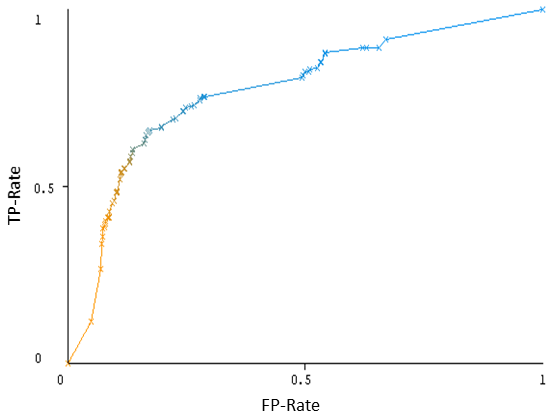
\includegraphics[width=0.25\linewidth]{images/j48_feat}} 
  \subfloat[][LR\\AUC = $0,62$]{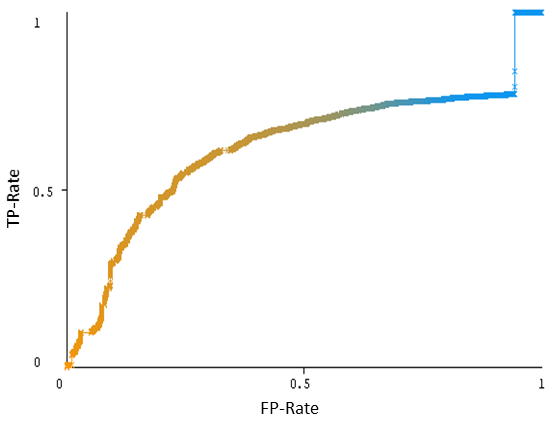
\includegraphics[width=0.25\linewidth]{images/lr_feat}}
  \subfloat[][NN\\AUC = $0,61$]{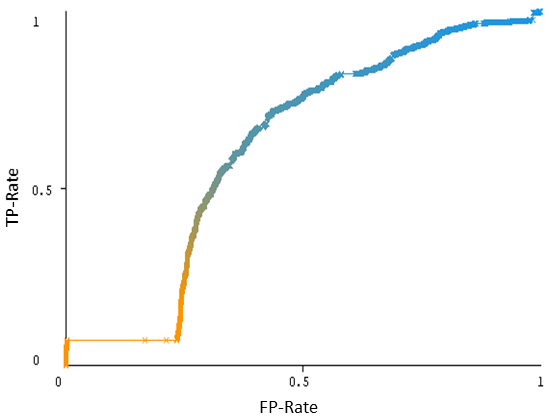
\includegraphics[width=0.25\linewidth]{images/nn_feat}}
  \subfloat[][SGD\\AUC = $0,53$]{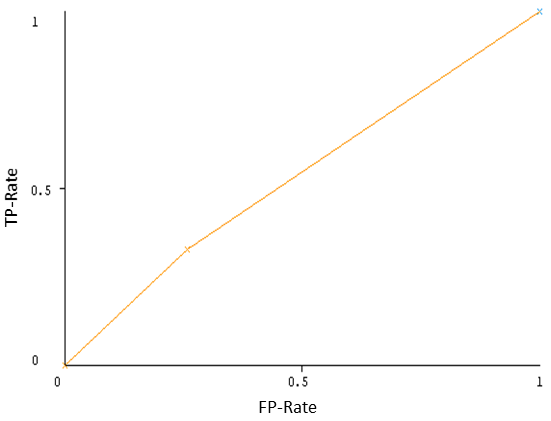
\includegraphics[width=0.25\linewidth]{images/sgd_feat}}
  \qquad
  \subfloat[][KNN\\AUC = $0,73$]{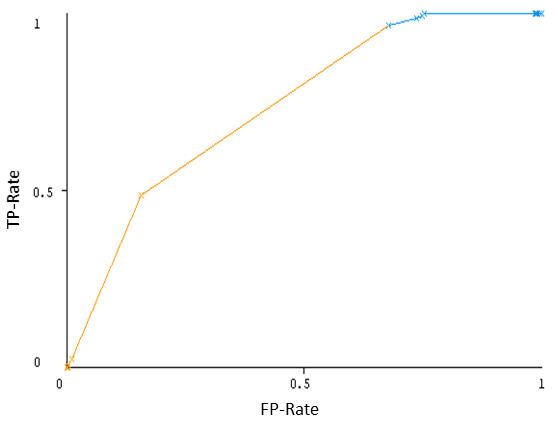
\includegraphics[width=0.25\linewidth]{images/knn_feat}}
  \subfloat[][NB\\AUC = $0,80$]{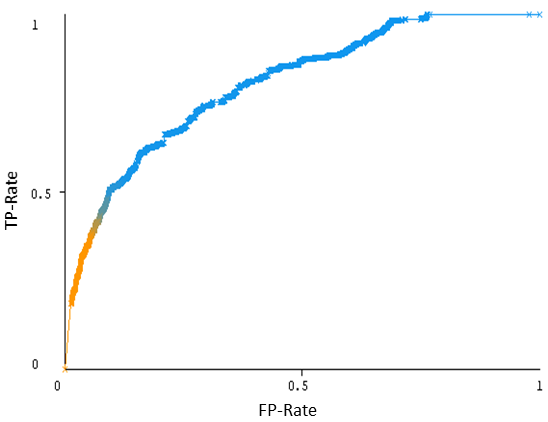
\includegraphics[width=0.25\linewidth]{images/nb_feat}}
  \subfloat[][RF\\AUC = $0,84$]{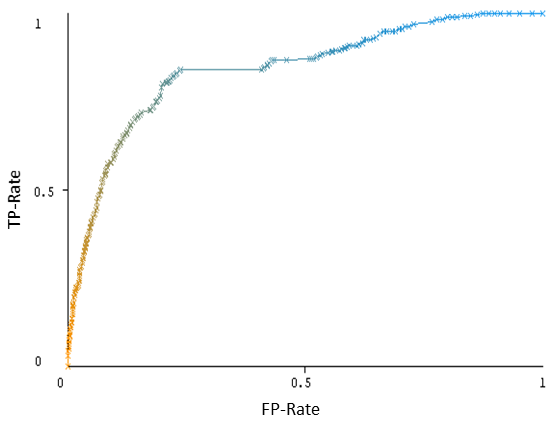
\includegraphics[width=0.25\linewidth]{images/rf_feat}} 
  \subfloat[][SVM\\AUC = $0,49$]{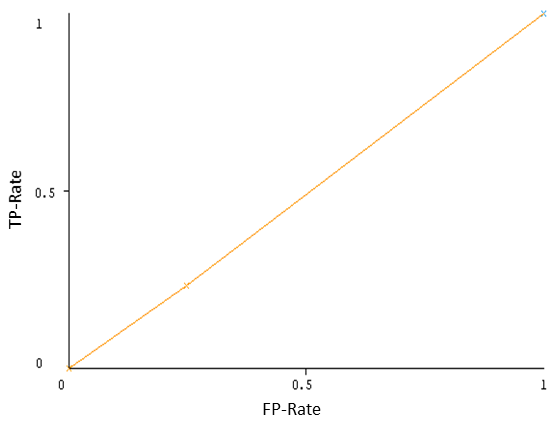
\includegraphics[width=0.25\linewidth]{images/svm_feat}}
  \caption{ROC-Kurven des featurebasierten Datensets \label{fig:roc-feat}}
\end{figure}

Es ist zu erkennen, dass keine ROC-Kurve den in \hyperref[roc-def]{Abschnitt 5.2.1} vorgestellten Idealfall annähert. Die beste Vorhersageperformanz zeigt erneut der RF-Klassifikator mit einem ROC-Bereich von $0,84$. Der NB-Klassifikator zeigt eine minimal geringere Performanz mit einem ROC-Bereich von $0,80$. Eine durchschnittliche Performanz von $0,77$ beziehungsweise $0,72$, bezogen auf den ROC-Bereich, weisen die Klassifikatoren J48 und KNN auf. Die Performanz der LR- und NN-Klassifikatoren liegen im unteren Durchschnitt. Den unerwünschten Fall einer winkelhalbierenden ROC-Kurve zeigen die SGD- und SVM-Klassifikatoren. Dies spiegeln auch die ROC-Bereiche wider. Sie \glqq raten\grqq{} also, statt präzise Vorhersagen zu treffen.

\paragraph{Zusammenfassung}
In jeder der betrachteten Kategorien von Metriken erwiesen sich die Ent-scheidungsbaum-basierten Klassifikatoren J48 und RF als am performantesten im Vergleich zu den weiteren Klassifikatoren. Der RF-Klassifikator erreichte dabei meist zudem eine etwas höhere Performanz. Die den Klassifikatoren zugrundeliegenden Algorithmen scheinen das gegebene featurebasierte Datenset mit seinen elf Attributen, hinsichtlich der Entwicklung der Ableitungsfunktion zur Vorhersage neuer Daten, am besten verarbeiten zu können.
Die Klassifikatoren SGD und SVM zeigten für jede Kategorie von Evaluationsmetriken stets die im Vergleich schlechtesten Performanzen. Es wurde zudem festgestellt, dass die Klassifikatoren raten, statt Vorhersagen zu treffen. Das featurebasierte Datenset scheint somit für diese Klassifikationsalgorithmen nicht geeignet zu sein. Gründe dafür können eine zu geringe Anzahl an Instanzen oder eine zu hohe Anzahl an Attributen sein.

\fbox{\parbox{\linewidth}{RQ3b: WELCHE ERGEBNISSE KÖNNEN BEI DER VORHERSAGE VON FEHLERHAFTEN ODER FEHLERFREIEN FEATURES ERZIELT WERDEN?\medskip\\
Es konnte gezeigt werden, dass die Entscheidungsbaum-basierten Klassifikatoren J48 und RF mit Accuracies von $84\%$ die höchste Performanz der acht Klassifikatoren aufweisen. Die weiteren Evaluationsmetriken bestätigten diese Ergebnisse. Die Klassifikatoren SGD und SVM zeigten die im Vergleich schlechtesten Performanzergebnisse.}}

\subsection{Ergebnisse und Vergleich der dateibasierten Klassifikatoren}
\label{classic-eval}

Dieser Abschnitt dient zur Evaluation und zum Vergleich der Klassifikatoren der dateibasierten Datensets, deren Erstellung in \hyperref[new-datasets]{Abschnitt 3.3} erläutert wurde. Der Grund dieses Vergleiches ist die Messung der Einflüsse der featurebasierten Metriken auf die Vorhersagen einer klassischen dateibasierten Methode, die der wissenschaftlichen Literatur entnommen wurde \cite{Moser2008}. Die Aufteilung dieses Abschnitts ist analog zum vorherigen Abschnitt. Darüber hinaus wird die folgende Forschungsfrage im Fließtext sowie zusammengefasst am Ende des Abschnitts beantwortet:
\vspace{-\topsep}
\begin{itemize}
\setlength{\itemsep}{-2pt}
 \item RQ3d: Wie beeinflusst die Verwendung von featurebasierten Metriken die dateibasierte Fehlervorhersage?
\end{itemize} 

Durch die Betrachtung der Ergebnisse der Evaluationsmetriken beider Datensets, kann der Einfluss der featurebasierten Metriken im erweiterten dateibasierten Datensets auf die Performanz der Vorhersagen analysiert werden. 

\paragraph{Konfusionsmatrizen}
Die Konfusionsmatrizen der dateibasierten Datensets sind in \autoref{tab:mat-eval} aufgeführt. Die übergeordneten Spalten sind dabei in das \glqq einfache\grqq{} und das erweiterte Datenset angeordnet. Beide Datensets umfassen die selbe Anzahl an Datensätzen, somit sind die \glqq total\grqq -Spalten identisch.
Eine kurze Analyse der \glqq defekt\grqq - \glqq Realität defekt\grqq - Felder zeigt, dass nur sehr wenige tatsächlich defekten Datenpunkte auch wirklich als defekt vorhergesagt wurden. Dies spiegelt sich auch in den weiteren Ergebnissen der Evaluationsmetriken wider.

\begin{table}[h!t]
\centering
\caption{Konfusionsmatrizen der dateibasierten Datensets}
\label{tab:mat-eval}
\resizebox{\linewidth}{!}{%
\begin{tabular}{|>{\hspace{0pt}}p{0.075\linewidth}>{\hspace{0pt}}p{0.231\linewidth}|>{\RaggedLeft\hspace{0pt}}p{0.1\linewidth}>{\RaggedLeft\hspace{0pt}}p{0.135\linewidth}>{\RaggedLeft\hspace{0pt}}p{0.1\linewidth}|>{\RaggedLeft\hspace{0pt}}p{0.102\linewidth}>{\RaggedLeft\hspace{0pt}}p{0.137\linewidth}>{\RaggedLeft\hspace{0pt}}p{0.104\linewidth}|} 
\cline{3-8}
\multicolumn{1}{>{\hspace{0pt}}p{0.075\linewidth}}{}            &                                    & \multicolumn{3}{>{\Centering\hspace{0pt}}p{0.335\linewidth}|}{\textbf{\glqq einfaches\grqq{} dateibasiertes Datenset}} & \multicolumn{3}{>{\Centering\hspace{0pt}}p{0.343\linewidth}|}{\textbf{erweitertes dateibasiertes Datenset}}  \\ 
\cline{2-8}
\multicolumn{1}{>{\Centering\hspace{0pt}}p{0.075\linewidth}|}{} & \textbf{Ermittelt -\textgreater{}} & \textbf{defekt} & \textbf{fehlerfrei} & \textbf{total}                                & \textbf{defekt} & \textbf{fehlerfrei} & \textbf{total}                                        \\ 
\hline
\multirow{3}{0.075\linewidth}{\hspace{0pt}J48}                   & Realität defekt                    & $11$              & $102$                 & $113$                                           & $15$              & $98$                  & $113$                                                   \\
                                                                & Realität fehlerfrei                & $911$             & $20.923$              & $21.834$                                        & $1.120$           & $20.714$              & $21.834$                                                \\
                                                                & total                              & $922$             & $21.025$              & $21.947$                                        & $1.135$           & $2.0812$              & $21.947$                                                \\ 
\hline
\multirow{3}{0.075\linewidth}{\hspace{0pt}KNN}                  & Realität defekt                    & $29$              & $84$                  & $113$                                           & $20$              & $93$                  & $113$                                                   \\
                                                                & Realität fehlerfrei                & $5.209$           & $16.625$              & $21.834$                                        & $4.861$           & $16.973$              & $21.834$                                                \\
                                                                & total                              & $5.238$           & $16.709$              & $21.947$                                        & $4.881$           & $17.066$              & $21.947$                                                \\ 
\hline
\multirow{3}{0.075\linewidth}{\hspace{0pt}LR}                   & Realität defekt                    & $36$              & $77$                  & $113$                                           & $32$              & $81$                  & $113$                                                   \\
                                                                & Realität fehlerfrei                & $2.520$           & $19.314$              & $21.834$                                        & $2.578$           & $19.256$              & $21.834$                                                \\
                                                                & total                              & $2.556$           & $19.391$              & $21.947$                                       & $2.610$           & $19.337$              & $21.947$                                                \\ 
\hline
\multirow{3}{0.075\linewidth}{\hspace{0pt}NB}                   & Realität defekt                    & $77$              & $36$                  & $113$                                           & $83$              & $30$                  & $113$                                                   \\
                                                                & Realität fehlerfrei                & $18.700$          & $3.134$               & $21.834$                                        & $18.750$          & $3.084$               & $21.834$                                                \\
                                                                & total                              & $18.777$          & $3.170$               & $21.947$                                        & $18.833$          & $3.114$               & $21.947$                                                \\ 
\hline
\multirow{3}{0.075\linewidth}{\hspace{0pt}NN}                   & Realität defekt                    & $6$               & $107$                 & $113$                                           & $1$               & $112$                 & $113$                                                   \\
                                                                & Realität fehlerfrei                & $4.341$           & $17.493$              & $21.834$                                        & $141$             & $21.693$              & $21.834$                                                \\
                                                                & total                              & $4.347$           & $17.600$              & $21.947$                                        & $142$             & $21.805$              & $21.947$                                                \\ 
\hline
\multirow{3}{0.075\linewidth}{\hspace{0pt}RF}                   & Realität defekt                    & $7$               & $106$                 & $113$                                           & $4$               & $109$                 & $113$                                                   \\
                                                                & Realität fehlerfrei                & $382$             & $21.452$              & $21.834$                                        & $366$             & $21.468$              & $21.834$                                                \\
                                                                & total                              & $389$             & $21.558$              & $21.947$                                        & $370$             & $21.577$              & $21.947$                                                \\ 
\hline
\multirow{3}{0.075\linewidth}{\hspace{0pt}SGD}                  & Realität defekt                    & $22$              & $91$                  & $113$                                           & $20$              & $93$                  & $113$                                                   \\
                                                                & Realität fehlerfrei                & $1.260$           & $20.574$              & $21.834$                                        & $1.226$           & $20.608$              & $21.834$                                                \\
                                                                & total                              & $1.282$           & $20.665$              & $21.947$                                        & $1.246$           & $20.701$              & $21.947$                                                \\ 
\hline
\multirow{3}{0.075\linewidth}{\hspace{0pt}SVM}                  & Realität defekt                    & $22$              & $91$                  & $113$                                           & $21$              & $92$                  & $113$                                                   \\
                                                                & Realität fehlerfrei                & $1.041$           & $20.793$              & $21.834$                                        & $991$             & $20.843$              & $21.834$                                                \\
                                                                & total                              & $1.063$           & $20.884$              & $21.947$                                        & $1.012$           & $20.935$              & $21.947$                                                \\
\hline
\end{tabular}
}
\end{table}

\paragraph{Accuracies}

Die Accuracies der Klassifikatoren der dateibasierten Datensets sind in \autoref{fig:final-eval} dargestellt. Die konkreten Zahlenwerte können dem \hyperref[appendix2]{Anhang} entnommen werden.

\begin{figure}[h!t]
    \centering
    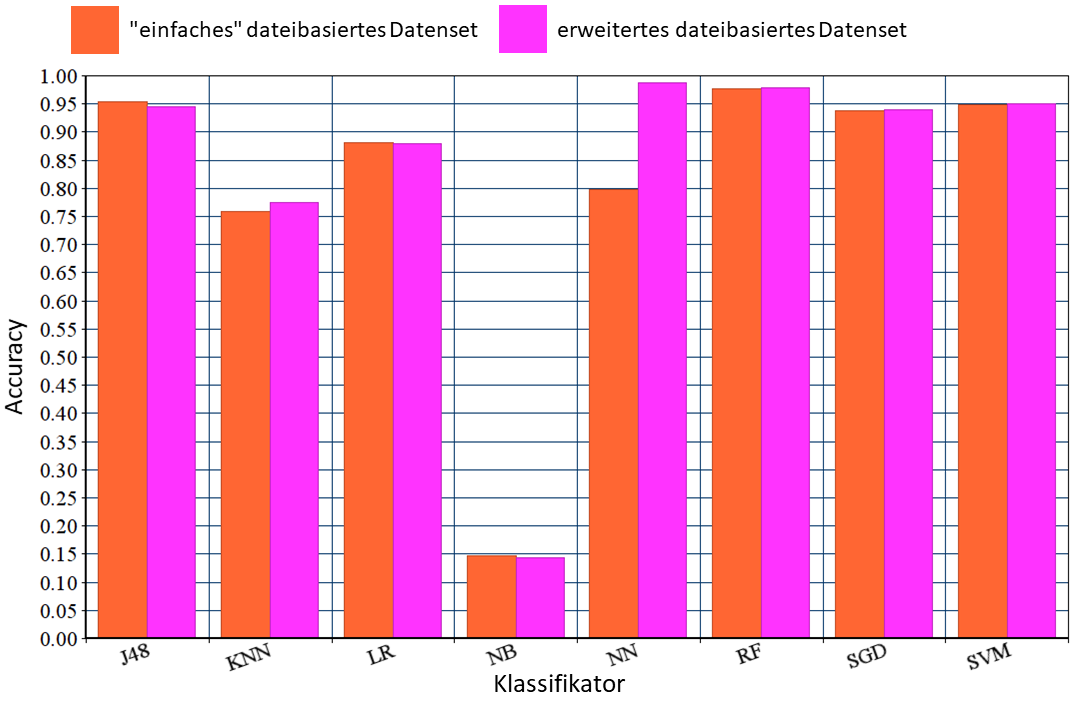
\includegraphics[width=\textwidth]{images/final_eval}
    \caption{Vergleich der Accuracies der dateibasierten Datensets\label{fig:final-eval}}
\end{figure}

Der Vergleich zwischen den Datensets zeigt, dass die Einbindung der featurebasierten Metriken für sechs von acht Klassifikatoren keinen signifikanten Einfluss auf die Performanz der Vorhersagen hat. Die erzielten Werte der Accuracies sind dort jeweils auf dem selben Niveau. Mit etwa $15\%$ Treffergenauigkeit erzielt der NB-Klassifikator die im Vergleich schlechteste Accuracy. Dieser scheint die hohe Anzahl an Datensätzen nicht korrekt verarbeiten zu können. Die Klassifikatoren KNN und LR erreichten mit etwa $76\%$ beziehungsweise $87\%$ überdurchschnittlich hohe Ergebnisse. Mit Werten von über $90\%$ besitzen die Klassifikatoren J48, RF, SGD und SVM äußerst hohe Werte, deren Aussagekraft zunächst infrage gestellt werden sollten. Eine Betrachtung der weiteren Evaluationsmetriken sollte vorgenommen werden.
Eine Auffälligkeit zeigt der NN-Klassifikator. Es ist ein deutlicher Sprung der Werte von etwa $18\%$ zwischen dem \glqq einfachen\grqq{} und dem erweiterten Datenset zu erkennen. Diese Auffälligkeit sollte ebenfalls anhand der weiteren Evaluationsmetriken analysiert und interpretiert werden. Sie kann einerseits verdeutlichen, dass der Klassifikator des erweiterten Datensets durch die Hinzunahme der zusätzlichen Attribute genauere Vorhersagen treffen kann oder durch diesen Umstand die Vorhersagen negativ beeinflusst werden, sodass die Ergebnisse verzerrt werden.

\paragraph{TP-Rate / Recall, FP-Rate, Precision, F-Score}
Dieser Abschnitt stellt die Ergebnisse der weiteren Evaluationsmetriken der dateibasierten Datensets in \autoref{tab:met-results} vor. Die übergeordneten Spalten werden erneut durch die beiden Datensets repräsentiert. Die vollständigen Tabellen der Ergebnisse der Evaluation, inklusive einer weiteren Metrik, können im \hyperref[appendix3]{Anhang} gefunden werden.

\begin{table}[h!t]
\centering
\caption{Ergebnisse der Evaluationsmetriken der dateibasierten Datensets (TPR = TP-Rate)}
\label{tab:met-results}
\resizebox{\linewidth}{!}{%
\begin{tabular}{|ll|rrr|rrr|} 
\cline{3-8}
\multicolumn{1}{l}{} &              & \multicolumn{3}{c|}{\textbf{\glqq einfaches\grqq{} dateibasiertes Datenset} } & \multicolumn{3}{c|}{\textbf{erweitertes dateibasiertes Datenset} }  \\ 
\cline{3-8}
\multicolumn{1}{l}{} &              & \textbf{defekt}  & \textbf{fehlerfrei}  & \textbf{Mittel}          & \textbf{defekt}  & \textbf{fehlerfrei}  & \textbf{Mittel}           \\ 
\hline
\multirow{4}{*}{J48} & TPR / Recall & $0,10$             & $0,96$                 & $0,53$                     & $0,13$             & $0,95$                 & $0,54$                      \\
                     & FP-Rate      & $0,04$             & $0,90$                 & $0,47$                     & $0,05$             & $0,87$                 & $0,46$                      \\
                     & Precision    & $0,01$             & $1,00$                 & $0,51$                     & $0,01$             & $1,00$                 & $0,51$                      \\
                     & F-Score      & $0,02$             & $0,98$                 & $0,50$                     & $0,02$             & $0,97$                 & $0,50$                      \\ 
\hline
\multirow{4}{*}{KNN} & TPR / Recall & $0,26$             & $0,76$                 & $0,51$                     & $0,18$             & $0,78$                 & $0,48$                      \\
                     & FP-Rate      & $0,24$             & $0,74$                 & $0,49$                     & $0,22$             & $0,82$                 & $0,47$                      \\
                     & Precision    & $0,01$             & $1,00$                 & $0,51$                     & $0,00$             & $1,00$                 & $0,50$                      \\
                     & F-Score      & $0,01$             & $0,86$                 & $0,44$                     & $0,01$             & $0,87$                 & $0,44$                      \\ 
\hline
\multirow{4}{*}{LR}  & TPR / Recall & $0,32$             & $0,89$                 & $0,61$                     & $0,28$             & $0,88$                 & $0,58$                      \\
                     & FP-Rate      & $0,12$             & $0,68$                 & $0,40$                     & $0,12$             & $0,72$                 & $0,42$                      \\
                     & Precision    & $0,01$             & $1,00$                 & $0,51$                     & $0,01$             & $1,00$                 & $0,51$                      \\
                     & F-Score      & $0,03$             & $0,94$                 & $0,49$                     & $0,02$             & $0,94$                 & $0,48$                      \\ 
\hline
\multirow{4}{*}{NB}  & TPR / Recall & $0,68$             & $0,14$                 & $0,41$                     & $0,74$             & $0,14$                 & $0,44$                      \\
                     & FP-Rate      & $0,86$             & $0,32$                 & $0,59$                     & $0,86$             & $0,27$                 & $0,57$                      \\
                     & Precision    & $0,00$             & $0,99$                 & $0,50$                     & $0,00$             & $0,99$                 & $0,50$                      \\
                     & F-Score      & $0,01$             & $0,25$                 & $0,13$                     & $0,01$             & $0,25$                 & $0,13$                      \\ 
\hline
\multirow{4}{*}{NN}  & TPR / Recall & $0,05$             & $0,80$                 & $0,43$                     & $0,01$             & $0,99$                 & $0,50$                      \\
                     & FP-Rate      & $0,20$             & $0,95$                 & $0,58$                     & $0,01$             & $0,99$                 & $0,50$                      \\
                     & Precision    & $0,00$             & $0,99$                 & $0,50$                     & $0,01$             & $1,00$                 & $0,51$                      \\
                     & F-Score      & $0,00$             & $0,89$                 & $0,45$                     & $0,01$             & $0,99$                 & $0,50$                      \\ 
\hline
\multirow{4}{*}{RF}  & TPR / Recall & $0,06$             & $0,98$                 & $0,52$                     & $0,04$             & $0,98$                 & $0,51$                      \\
                     & FP-Rate      & $0,02$             & $0,94$                 & $0,48$                     & $0,02$             & $0,97$                 & $0,50$                      \\
                     & Precision    & $0,02$             & $1,00$                 & $0,51$                     & $0,01$             & $1,00$                 & $0,51$                      \\
                     & F-Score      & $0,03$             & $0,90$                 & $0,47$                     & $0,02$             & $0,99$                 & $0,51$                      \\ 
\hline
\multirow{4}{*}{SGD} & TPR / Recall & $0,20$             & $0,94$                 & $0,57$                     & $0,18$             & $0,94$                 & $0,56$                      \\
                     & FP-Rate      & $0,06$             & $0,81$                 & $0,44$                     & $0,06$             & $0,82$                 & $0,44$                      \\
                     & Precision    & $0,02$             & $1,00$                 & $0,51$                     & $0,02$             & $1,00$                 & $0,51$                      \\
                     & F-Score      & $0,03$             & $0,97$                 & $0,50$                     & $0,03$             & $0,97$                 & $0,50$                      \\ 
\hline
\multirow{4}{*}{SVM} & TPR / Recall & $0,20$             & $0,95$                 & $0,58$                     & $0,19$             & $1,00$                 & $0,60$                      \\
                     & FP-Rate      & $0,05$             & $0,81$                 & $0,43$                     & $0,05$             & $0,81$                 & $0,43$                      \\
                     & Precision    & $0,02$             & $1,00$                 & $0,51$                     & $0,02$             & $1,00$                 & $0,51$                      \\
                     & F-Score      & $0,04$             & $0,97$                 & $0,51$                     & $0,04$             & $0,98$                 & $0,51$                      \\
\hline
\end{tabular}
}
\end{table}

Die Ergebnisse der weiteren Evaluationsmetriken beider Datensets zeigen erneut den Trend, dass nur wenige defekte Datenpunkte auch tatsächlich als defekt vorhergesagt wurden. Mit TP-Raten von $68\%$ beziehungsweise $74\%$ erreichten die NB-Klassifikatoren die höchsten Trefferquoten. Die weiteren Klassifikatoren liegen mit Werten von höchstens $32\%$ deutlich darunter. Die weiteren Metriken der \glqq defekt\grqq -Spalten repräsentieren ebenfalls äußerst schwache Ergebnisse. Auffällig sind die sehr hohen FP-Raten der NB-Klassifikatoren, die die guten Ergebnisse der TP-Raten deutlich abschwächen.

Die Werte der \glqq fehlerfrei\grqq -Spalten zeigen sehr gute Werte. Lediglich die jeweiligen FP-Raten mit über $68\%$ sind deutlich zu hoch und zeigen, dass die Klassifikatoren viele Datenpunkte inkorrekterweise als \glqq fehlerfrei\grqq{} vorhersagen. Eine Ausnahme davon bilden erneut die NB-Klassifikatoren, die zwar gute Werte bezüglich der FP-Raten und der Precision erzielten, allerdings Mängel bei den TP-Raten und folglich auch dem F-Score aufweisen. Zudem lassen sich die verschiedenen Accuracies der NN-Klassifikatoren mit den Ergebnissen der weiteren Evaluationsmetriken begründen. Es ist zu erkennen, dass sich zwischen den Datensets die Werte der TP-Raten und FP-Raten für beide Label unterscheiden. Infolgedessen weichen auch die F-Scores ab. Diese Abweichungen der Werte führen zu den unterschiedlichen Werten der Accuracies.

Die Mittelwerte zeigen, dass die Gesamtergebnisse durch die Werte der \glqq defekt\grqq{} -Spalten stark nach unten beeinflusst werden. Sie zeigen, dass alle Klassifikatoren auf einem durchschnittlichen bis unterdurchschnittlichen Niveau Vorhersagen treffen.

\paragraph{ROC-Kurven und -Bereiche}

Die ROC-Kurven samt ihrer zugehörigen ROC-Bereiche (als \glqq AUC\grqq{} vermerkt) der dateibasierten Datensets sind in \autoref{roc-file} zu sehen. Die dargestellten Farbverläufe der Kurven verdeutlichen erneut keine für diesen Zweck relevanten Informationen und können somit ignoriert werden.

Ein erster Blick auf die ROC-Kurven der Klassifikatoren zeigt ein relativ einheitliches Bild von Kurven, die sich sehr stark an der Winkelhalbierenden orientieren und zwischen den Datensets einheitlich sind. Mit der Ausnahme der RF Klassifikatoren beider Datensets zeigen die Kurven mit ihren zugehörigen ROC-Bereichen eine unterdurchschnittliche bis unerwünschte Performanz (\glqq Raten\grqq{} der Label) an. Mit einem ROC-Bereich von $0,71$ besitzen die RF-Klassifikatoren eine überdurchschnittliche Performanz im übergeordneten Vergleich.

Der Vergleich zwischen den NN-Klassifikatoren zeigt, dass der Klassifikator des einfachen Datensets das unerwünschte Verhalten zeigt und gleichzeitig inverse Vorhersagen trifft. Dies bedeutet, dass er in manchen Fällen statt dem Label \glqq fehlerfrei\grqq{} das Label \glqq defekt\grqq{} vorhersagt und umgekehrt. Die Kurve sowie der ROC-Bereich des Klassifikators des erweiterten Datensets zeigen hingegen nur das unerwünschte Verhalten in Form des \glqq Ratens\grqq{} der Vorhersagen. Dies zeigt, dass die in \autoref{fig:final-eval} dargestellten hohen Accuracies der NN-Klassifikatoren wahrscheinlich durch Zufall entstanden sind. In einer weiteren Anwendung der Testdaten hätten die Ergebnisse anders ausfallen können.

\begin{figure}[h!t]
  \centering
  \subfloat[][J48 einf.\\AUC = $0,61$]{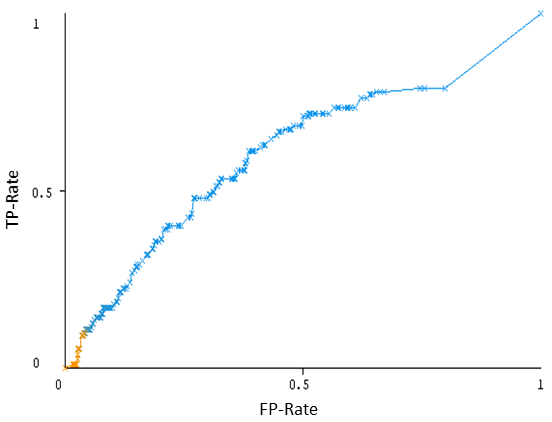
\includegraphics[width=0.25\linewidth]{images/j48_eval}} 
  \subfloat[][J48 erw.\\AUC = $0,61$]{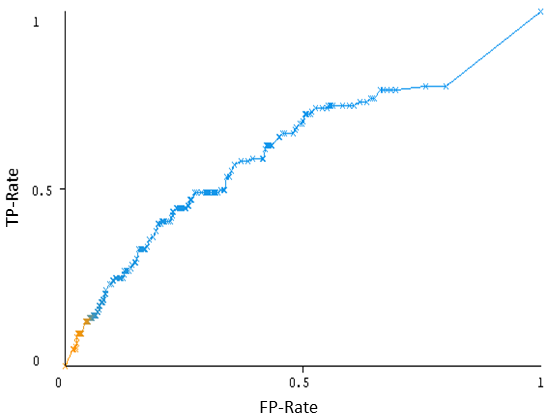
\includegraphics[width=0.25\linewidth]{images/j48_eval_feat}}
  \subfloat[][NN einf.\\AUC = $0,37$]{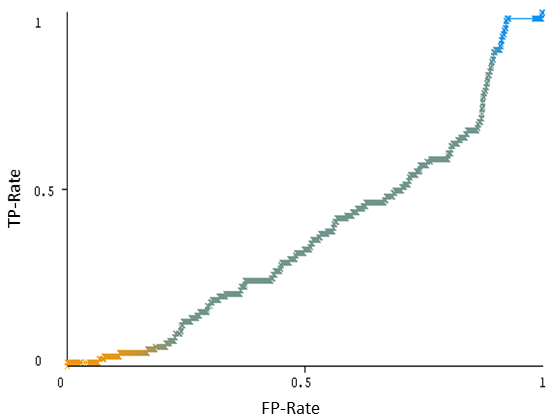
\includegraphics[width=0.25\linewidth]{images/nn_eval}}
  \subfloat[][NN erw.\\AUC = $0,54$]{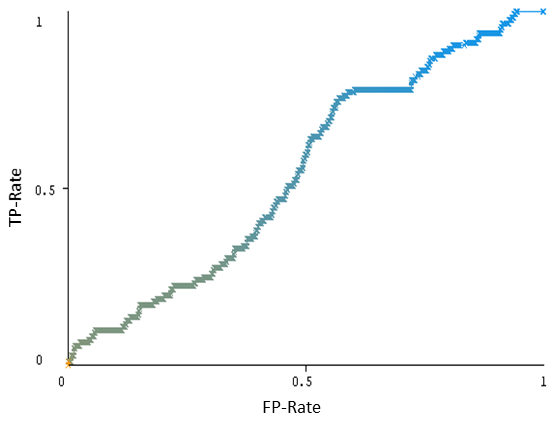
\includegraphics[width=0.25\linewidth]{images/nn_eval_feat}}
  \qquad
  \subfloat[][KNN einf.\\AUC = $0,55$]{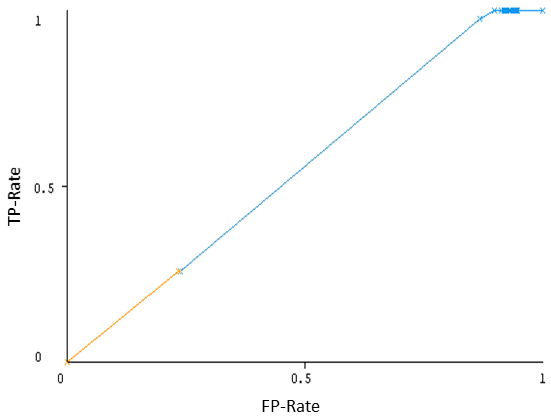
\includegraphics[width=0.25\linewidth]{images/knn_eval}}
  \subfloat[][KNN erw.\\AUC = $0,52$]{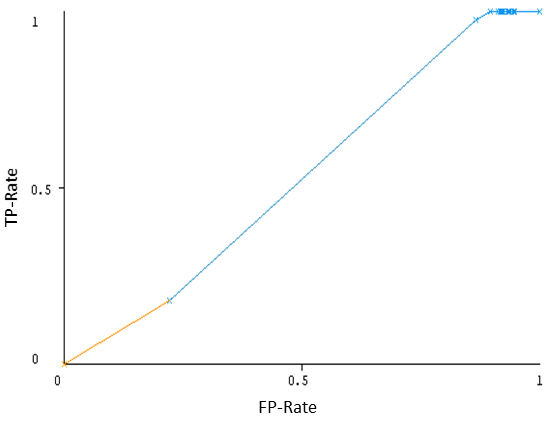
\includegraphics[width=0.25\linewidth]{images/knn_eval_feat}}
  \subfloat[][RF einf.\\AUC = $0,71$]{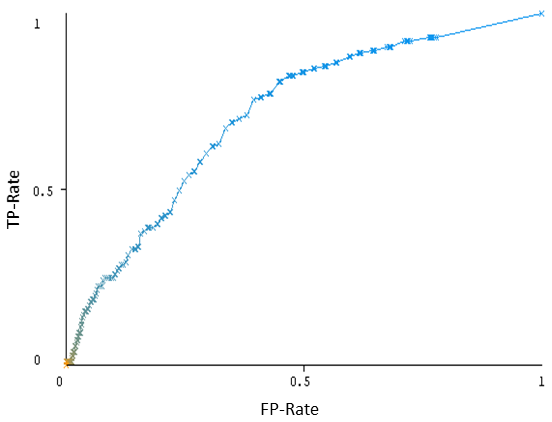
\includegraphics[width=0.25\linewidth]{images/rf_eval}} 
  \subfloat[][RF erw.\\AUC = $0,71$]{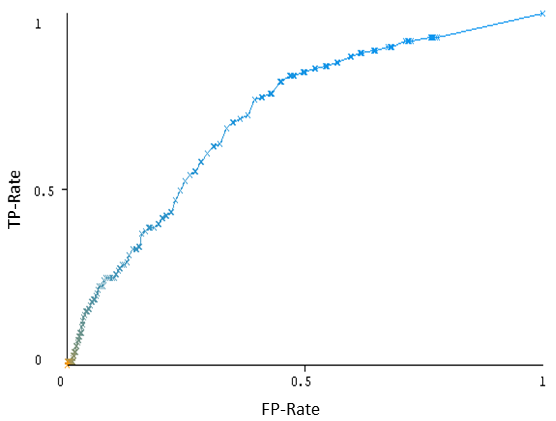
\includegraphics[width=0.25\linewidth]{images/rf_eval_feat}} 
  \qquad
  \subfloat[][LR einf.\\AUC = $0,65$]{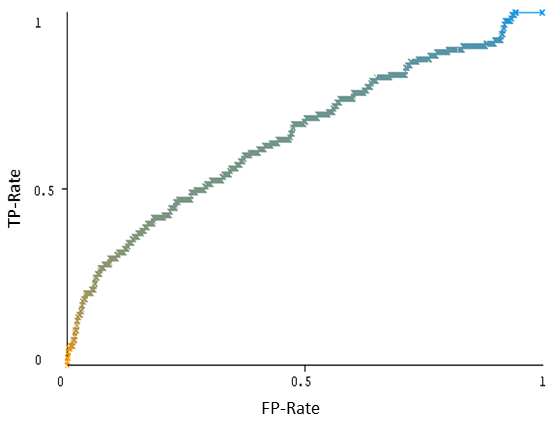
\includegraphics[width=0.25\linewidth]{images/lr_eval}}
  \subfloat[][LR erw.\\AUC = $0,62$]{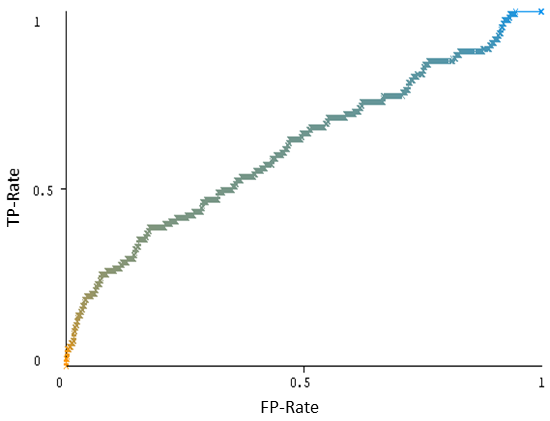
\includegraphics[width=0.25\linewidth]{images/lr_eval_feat}}
  \subfloat[][SGD einf.\\AUC = $0,57$]{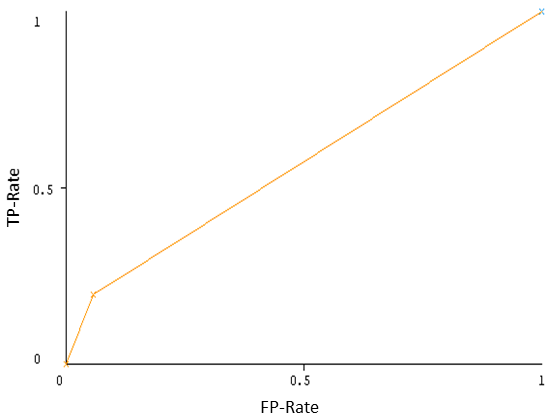
\includegraphics[width=0.25\linewidth]{images/sgd_eval}}
  \subfloat[][SGD erw.\\AUC = $0,56$]{\includegraphics[width=0.25\linewidth]{images/sgd_eval_feat}}
  \qquad
  \subfloat[][NB einf.\\AUC = $0,48$]{\includegraphics[width=0.25\linewidth]{images/nb_eval}}
  \subfloat[][NB erw.\\AUC = $0,47$]{\includegraphics[width=0.25\linewidth]{images/nb_eval_feat}}
  \subfloat[][SVM einf.\\AUC = $0,57$]{\includegraphics[width=0.25\linewidth]{images/svm_eval}}
  \subfloat[][SVM erw.\\AUC = $0,57$]{\includegraphics[width=0.25\linewidth]{images/svm_eval_feat}}
  \caption{ROC-Kurven der datenbasierten Datensets \label{roc-file}}
\end{figure}

\paragraph{Zusammenfassung}
Die Ergebnisse sämtlicher Metriken zeigten ein undifferenziertes und undeutliches Bild der Performanz der Klassifikatoren für beide Datensets. Der Grund für die gezeigten Ergebnisse ist die Unbalanciertheit der jeweiligen Testdatensets mit einem Anteil von \glqq defekt\grqq -Instanzen von nur $1\%$. Damit für dieses Label gute Ergebnisse erzielt werden können, müssen viele korrekte Vorhersagen der Klassifikatoren getroffen werden. Dies war jedoch für das vorhandene Testdatenset nicht der Fall, sodass viele Vorhersagen fälschlicherweise dem dominierenden Label \glqq fehlerfrei\grqq{} zugeordnet wurden, die dann allerdings infolgedessen hohe FP-Raten aufweisen. Diesen Umstand spiegeln auch die Mittelwerte in \autoref{tab:met-results} wider. Aufgrund der deutlich schwächeren Werte der \glqq defekt\grqq -Spalten, werden die Gesamtwerte, die durch den Mittelwert repräsentiert werden, nach unten beeinflusst. Wie jedoch schon in \hyperref[smote]{Abschnitt 4.2} erläutert wurde, ist es nicht vorgesehen, die Unbalanciertheit der Testdatensets mithilfe des SMOTE-Algorithmus auszugleichen.

Zusammenfassend lässt sich jedoch anhand der Ergebnisse der Tests der Klassifikatoren beider Datensets feststellen, dass der Einbezug der featurebasierten Metriken keinen nennenswert positiven Einfluss auf die Ergebnisse der dateibasierten Fehlervorhersage besitzt. Hinzugefügt werden muss jedoch, dass sie die Ergebnisse auch nicht negativ beeinflussen. Ein Grund dafür ist, dass die Auswahl an Attributen für beide dateibasierten Datensets sehr hoch ist. Das \glqq einfache\grqq{} Datenset umfasst 17 Attribute (+ Label) und das erweiterte Datenset umfasst 28 Attribute (+ Label). Eine Reduzierung der Attribute in Form einer Attributsauswahl könnte dazu beitragen, den Einfluss der featurebasierten näher zu analysieren. Die Attributsauswahl beschreibt einen automatisierten Prozess, welcher dazu dient, die optimale Anzahl und Auswahl von Attributen für das Training eines Klassifikators zu bestimmen. Die Durchführung einer solchen Attributsauswahl würde sich für zukünftige weiterführende Arbeiten anbieten.

\fbox{\parbox{\linewidth}{RQ3d: WIE BEEINFLUSST DIE VERWENDUNG VON FEATUREBASIERTEN METRIKEN DIE DATEIBASIERTE FEHLERVORHERSAGE?\medskip\\
Die Auswirkungen des Einbezugs der featurebasierten Metriken sind kaum messbar. Sowohl die Klassifikatoren des \glqq einfachen\grqq{} dateibasierten Datensets als auch die des erweiterten dateibasierten Datensets, erzielen die selben Ergebnisse mit geringen Abweichungen. Sie sind somit jeweils gleich performant bezüglich der Vorhersagen.}}

\section{Herausforderungen und Limitationen}

In diesem Abschnitt werden eine Reihe von Herausforderungen und Limitationen aufgezählt und erläutert, die im Rahmen der Erarbeitung der Forschungsziele auffällig wurden.

\subsection*{Identifikation von Features}

Die grundsätzliche Fragestellung, die im Rahmen der Identifikation der Features aufkam, war, was genau als Feature gezählt wird. Wie bereits in \hyperref[construction]{Abschnitt 3.2} erwähnt wurde, barg die Identifikation der Features einige Herausforderungen. So gestaltete sich die erste Herausforderung in der Ausfilterung von \glqq Header-Features\grqq{}, die in einigen Programmierparadigmen verwendet werden, um Header-Dateien im Sourcecode einzubinden. Diese Header-Features erzeugen jedoch keine Variabilität im Code, sodass sie unerwünscht sind. Identifizierbar waren die meisten dieser Header-Features an ihren vergebenen Namen, welche ein \texttt{\_h\_} aufwiesen. Auf diese Weise konnten sie mittels regulärer Ausdrücke schnell ermittelt und ausgefiltert werden. Es besteht jedoch auch die Möglichkeit, dass in einigen Softwareprojekten die Header-Features nicht explizit durch ihre Namensgebung kenntlich gemacht werden. Sie lassen sich somit nur schwer identifizieren, beispielsweise durch eine manuelle Sichtung der Kontexte der Features im Sourcecode. Dies wäre jedoch im vorliegenden Fall aufgrund der großen Menge an Features zeitaufwändig und wurde aus diesem Grund nicht durchgeführt. Die Entfernung der erkennbaren Header-Features zeigte, dass ein erheblicher Teil der zuvor identifizierten Features unerwünscht war. Diese Methode erwies sich somit als effektiv.
Eine Lösung, die zu dem genannten Problem beitragen könnte, wäre ein Tool zum Parsen von Sourcecode zur korrekten Identifikation von Features mittels automatisierter Analyse des Kontextes des Features. So würden auch die erwähnten \glqq falschen\grqq{} Features ermittelt werden. Ein solches Tool existiert momentan jedoch nicht. Verfügbare Tools zur Identifikation von Features verwenden reguläre Ausdrücke, die auch in dieser Arbeit verwendet wurden.

\subsection*{Einbindung des Bezugs zu Features}
Wie in \hyperref[dataset-creation]{Kapitel 3} festgestellt wurde, basiert der Bezug zu den Features auf den ihnen zugrundeliegenden Dateien. Dazu wurden die Diffs der veränderten Dateien analysiert. Ein Feature gilt somit als relevant, wenn es in einem Diff Erwähnung findet. Es kann jedoch auch vorkommen, dass der enthaltene Featurecode nicht an der im Diff beschriebenen Veränderung beteiligt war, sondern nur im als \glqq Hunk\grqq{} bezeichneten Teil des Diffs erwähnt wurde. Dieser bezeichnet einen Überhang des eigentlichen Kontexts der beschriebenen Veränderungen in Form von weiteren Codezeilen, die dieser Veränderung folgen. Es findet somit keine \glqq in-depth\grqq -Analyse des Sourcecodes statt. Dieser Weg wurde jedoch auch von der dieser Arbeit zugrundeliegenden wissenschaftlichen Arbeit gewählt \cite{Queiroz2016}. Ebenfalls werden die Metriken der Features auf Basis der Metadaten der zugrundeliegenden Dateien berechnet. Es findet somit eine Überapproximierung statt.

\subsection*{Heuristik zur Erkennung von korrektiven Commits}
\label{heuristic}

Die Heuristik zur Erkennung von korrektiven Commits wurde im Verlauf der Erarbeitung der Arbeit geändert. Zunächst wurde die gesamte Commit-Nachricht auf das Vorhandensein der Schlagworte analysiert. Dies führte jedoch dazu, dass einige Commits fälschlicherweise als korrektiv identifiziert wurden. Der Grund dafür war, dass die Commit-Nachrichten in einigen der verwendeten Softwareprojekte sehr umfangreich in der Anzahl der Wörter waren. In diesen Nachrichten wurden ausnahmslos alle Veränderungen, die mit den Commits vorgenommen wurden, erwähnt. Dabei handelte es sich jedoch meist um für diesen Zweck irrelevante Veränderungen. Es wurde festgestellt, dass sich die der Hauptgrund des Commits in der ersten Zeile der Commit-Nachricht befindet. Die Heuristik wurde daraufhin entsprechend angepasst, sodass nur noch die erste Zeile der Commit-Nachrichten betrachtet wurde. Eine Stichprobe von korrektiven Commits vor und nach der Anpassung der Heuristik zeigte, dass die Veränderung dazu führte, dass tatsächlich irrelevante korrektive Commits entfernt wurden.

\subsection*{Unpräzisiertheit des SZZ-Algorithmus}

Eine Limitation, die im Laufe der Erstellung des Datensets durch Literaturrecherchen festgestellt wurde, bezieht sich auf den SZZ-Algorithmus. Dieser wurde genutzt, um fehlereinführende Commits auf Basis der Commit-Hashes der korrektiven Commits zu identifizieren. Analysen des Algorithmus ergaben, dass momentan verfügbare Implementationen und somit auch die des verwendeten Python-Tools PyDriller lediglich etwa 69\% der tatsächlich existierenden fehlereinführenden Commits identifizieren können \cite{Wen2019}. Darüber hinaus wurde herausgefunden, dass etwa $64\%$ der identifizierten Commits falsch ermittelt wurden \cite{Wen2019}. Der Algorithmus gilt somit als unpräzise \cite{Wen2019}. Die Begründung dafür lautet wie folgt:

\begin{quotation}
The reason is that the implicit assumptions of the SZZ algorithm
are violated by the insufficient file coverage and statement direct
coverage between bug-inducing and bug-fixing commits. - \cite{Wen2019}
\medskip \\
\textit{Der Grund dafür ist, dass die impliziten Annahmen des SZZ-Algorithmus durch die unzureichende \glqq file coverage\grqq{} und die unzureichende \glqq statement direct
coverage\grqq{} der Aussage zwischen fehlereinführenden und korrektiven Commits verletzt werden.}
\end{quotation}

Ferner stellten die Autoren der Studie in eigenen durchgeführten Tests fest, dass die Ergebnisse von acht aus zehn früheren Studien durch den unpräzisen Algorithmus signifikant beeinflusst wurden \cite{Wen2019}. Dies kann somit auch auf diese Arbeit zutreffen, wurde jedoch nicht weiter analysiert. Es existiert jedoch momentan keine alternative Methode zur Identifizierung von fehlereinführenden Commits. Sollte eine neue Methode oder eine verbesserte Version des SZZ-Algorithmus veröffentlicht werden, so würde es sich anbieten, die Hauptschritte dieser Arbeit unter Berücksichtigung der neuen Methode zu wiederholen, um sie mit den hier vorliegenden Ergebnissen zu vergleichen. So könnten die Einflüsse des neuen SZZ-Algorithmus herausgestellt werden.

\subsection*{Unzureichende Metadaten von xfig}
\label{xfig}
Im Rahmen der Identifizierung der korrektiven Commits wurde festgestellt, dass für das Softwareprojekt \glqq xfig\grqq{} keine Ergebnisse erzielt werden konnten. Folglich konnten keine fehlereinführenden Commits festgestellt werden. Zu sehen ist dies auch in \autoref{tab:tools-values2}. Der Grund für die fehlende Identifizierung der korrektiven Commits ist, dass die Commit-Nachrichten des Softwareprojekts keines der festgelegten Schlagworte enthalten. Sie bestehen lediglich aus der Angabe der Nummer des mit dem Commit freigegebenen Releases. Beispiele dafür sind:

\begin{itemize}
\setlength{\itemsep}{-2pt}
\item Commit: \texttt{af30126616c5c5a8db3ba017dedbcbdf48fbc528}\\Nachricht: \texttt{xfig-3.2.7b}
\item Commit: \texttt{a444a8ae7995dbfd2ebce4696ed2cca7ad33b6e1}\\Nachricht: \texttt{xfig-3.2.6.tar.xz}
\item Commit: \texttt{f3706bcafe9049247eee1a88d64f9f8b4e98c076}\\Nachricht: \texttt{xfig.3.0.tar.gz}
\end{itemize}

Der Umstand, dass weder korrektive noch fehlereinführende Commits identifiziert wurden, führt dazu, dass jedes Feature und jede Datei automatisch als \glqq fehlerfrei\grqq{} eingestuft wird. Dabei finden jedoch einige Zuordnungen inkorrekt statt. In Anbetracht dieser Tatsache wurde entschieden, \glqq xfig\grqq{} bei der Zusammenstellung der finalen Datensets nicht mit einzubinden.

\subsection*{Vorhersageziel}
Die Festlegung des Vorhersageziels war bis zum Ende der sechsmonatigen Bearbeitungszeit dieser Arbeit stets ein Diskussionsthema zwischen den beteiligten Personen. Wie im Kapitel zur Erstellung der Datensets bereits gezeigt wurde, sind die Werte der Metriken der Features und Dateien für jedes Datenset nach Releases in Form des Mittelwertes aggregiert. Somit läge es auch nahe, zukünftige Releases als den Input neuer Daten zur Vorhersage zu verwenden. Es werden dann also defekte Features oder Dateien in einem Release vorhergesagt. Eine weitere Möglichkeit liegt in der Betrachtung von Commits. Dazu müssen jedoch die Metriken vom Release-Level auf ein Commit-Level abstrahiert werden.

Eine Literaturrecherche in früheren wissenschaftlichen Arbeiten zum Thema der Fehlervorhersage zeigte, dass die Vorhersage auf Release-Level die überwiegend genutzte Option ist (siehe \cite{Queiroz2016,Zimmermann2007,Moser2008,Dhiauddin2012,Wang2012,Li2017}). Die Vorhersage auf Release-Level gilt infolgedessen als valide Methode und wird somit auch für diese Arbeit übernommen. Je nach Kontext werden somit defekte oder fehlerfreie Features beziehungsweise Dateien auf \emph{Release-Level} vorhergesagt. Anzumerken ist, dass die Vorhersage auf Post-Release-Level stattfindet, da die Festlegung, ob eine Datei oder ein Feature defekt oder fehlerfrei ist, auf Basis der letzten Commits eines Releases geschieht (siehe Anmerkungen in \hyperref[label-explanation]{Abschnitt 3.3}).

Die Aggregation der Metriken auf Release-Level bietet zudem den Vorteil, dass so wesentlich aussagekräftigere Werte erreicht werden können, ala auf Commit-Level \cite{Zimmermann2007}. Ein Beispiel dafür ist die Metrik \texttt{ADEV} des featurebasierten Datensets, welches die Anzahl der beteiligten Entwickler an einem Feature beziehungsweise an einer Datei angibt. Auf Commit-Level wäre dieser Wert stets 1, da das Versionierungssystem Git nur einen Commit-Autor zulässt. Eine Aggregation über mehrere Commits eines Releases liefert wesentlich differenzierte und aussagekräftigere Werte.

\cleardoublepage

%Um ein differenzierteres Bild der Performanz der Klassifikatoren zu erhalten, wurde eine weitere Testmethode als Alternative zur Aufteilung der Datensets in Training- und Testdaten hinzugezogen. Dabei handelt es sich um die sogenannte \glqq \texttt{n}-fold-cross-validation\grqq. Bei dieser Methode werden die Trainingsdaten in \texttt{n} gleich große Datenmengen (\glqq folds\grqq) aufgeteilt, welche dann jeweils mit einer Split-Ratio von $90:10$ zum Training der einzelnen Klassifikatoren dienen \cite{IanWitten}. Die Ergebnisse der Evaluationsmetriken bilden sich dann aus dem Mittelwert der Einzelergebnisse der \texttt{n} Vorgänge \cite{IanWitten}. Diese Methode findet auch in der wissenschaftlichen Literatur Anwendung (zum Beispiel \cite{Alam2013,Chawla2002,Alsaeedi2019}). Für diesen Fall wird eine 10-fold-cross-validation durchgeführt. Die Ergebnisse der Evaluationsmetriken sind in \autoref{tab:kx} aufgeführt. Ein Überblick über die Ergebnisse zeigt, dass diese wesentlich differenzierter und nachvollziehbarer ausgefallen sind sowie keine signifikanten Unterschiede zwischen den Datensets aufweisen. Es zeigt sich, dass die beiden Entscheidungsbaum-basierten Klassifikatoren J48 und RF die im Vergleich höchste Performanz mit einer Accuracy von $96\%$ beziehungsweise $98\%$ besitzen. Die FP-Rate der Klassifikatoren ist außerdem äußerst gering. Gleiches zeigt sich für den KNN-Klassifikator. Die weiteren Ergebnisse der Metriken bestätigen die hohe Performanz. Die Klassifikatoren SGD und SVM zeigen anhand ihrer ROC-Bereiche (siehe ROC-Area), dass sie unerwünschte Vorhersagen in Form des \glqq Ratens\grqq{} durchführen. Auffällig ist, dass die Werte zwischen den NN-Klassifikatoren beider Datensets nicht mehr abweichen. Beide Klassifikatoren arbeiten wie die weiteren, bisher unerwähnten, Klassifikatoren auf einem durchschnittlichen Niveau.
%
%\begin{table}[ht]
%\centering
%\caption{Ergebnisse der Evaluationsmetriken auf Basis der 10-fold-cross-validation (TPR = TP-Rate, Rec. = Recall)}
%\label{tab:kx}
%\resizebox{\linewidth}{!}{%
%\begin{tabular}{|>{\hspace{0pt}}p{0.06\linewidth}>{\hspace{0pt}}p{0.119\linewidth}|>{\RaggedLeft\hspace{0pt}}p{0.123\linewidth}>{\RaggedLeft\hspace{0pt}}p{0.17\linewidth}>{\RaggedLeft\hspace{0pt}}p{0.112\linewidth}|>{\RaggedLeft\hspace{0pt}}p{0.121\linewidth}>{\RaggedLeft\hspace{0pt}}p{0.168\linewidth}>{\RaggedLeft\hspace{0pt}}p{0.112\linewidth}|} 
%\cline{3-8}
%\multicolumn{1}{>{\hspace{0pt}}p{0.06\linewidth}}{} &           & \multicolumn{3}{>{\Centering\hspace{0pt}}p{0.405\linewidth}|}{\textbf{\glqq einfaches\grqq{} dateibasiertes Datenset} } & \multicolumn{3}{>{\Centering\hspace{0pt}}p{0.401\linewidth}|}{\textbf{erweitertes dateibasiertes Datenset} }  \\ 
%\cline{3-8}
%\multicolumn{1}{>{\hspace{0pt}}p{0.06\linewidth}}{} &           & \textbf{defekt}  & \textbf{fehlerfrei}                                 & \textbf{Mittel}                     & \textbf{defekt}  & \textbf{fehlerfrei}                                 & \textbf{Mittel}                      \\ 
%\hline
%\multirow{6}{0.06\linewidth}{\hspace{0pt}J48}       & Accuracy  & \multicolumn{2}{>{\RaggedLeft\hspace{0pt}}p{0.293\linewidth}}{gesamt:} & $0,96$                                & \multicolumn{2}{>{\RaggedLeft\hspace{0pt}}p{0.289\linewidth}}{gesamt:} & $0,96$                                 \\
%                                                    & TPR/Rec.  & $0,94$             & $0,97$                                                & $0,96$                                & $0,94$             & $0,97$                                                & $0,96$                                 \\
%                                                    & FP-Rate   & $0,03$             & $0,06$                                                & $0,05$                                & $0,03$             & $0,06$                                                & $0,05$                                 \\
%                                                    & Precision & $0,96$             & $0,96$                                                & $0,96$                                & $0,96$             & $0,96$                                                & $0,86$                                 \\
%                                                    & F-Score   & $0,95$             & $0,97$                                                & $0,96$                                & $0,95$             & $0,96$                                                & $0,96$                                 \\
%                                                    & ROC-Area  & $0,97$             & $0,97$                                                & $0,97$                                & $0,97$             & $0,97$                                                & $0,97$                                 \\ 
%\hline
%\multirow{6}{0.06\linewidth}{\hspace{0pt}KNN}       & Accuracy  & \multicolumn{2}{>{\RaggedLeft\hspace{0pt}}p{0.293\linewidth}}{gesamt:} & $0,91$                                & \multicolumn{2}{>{\RaggedLeft\hspace{0pt}}p{0.289\linewidth}}{gesamt:} & $0,91$                                 \\
%                                                    & TPR/Rec.  & $0,87$             & $0,94$                                                & $0,91$                                & $0,87$             & $0,94$                                                & $0,91$                                 \\
%                                                    & FP-Rate   & $0,06$             & $0,13$                                                & $0,10$                                & $0,06$             & $0,13$                                                & $0,10$                                 \\
%                                                    & Precision & $0,92$             & $0,91$                                                & $0,92$                                & $0,91$             & $0,91$                                                & $0,91$                                 \\
%                                                    & F-Score   & $0,89$             & $0,93$                                                & $0,91$                                & $0,89$             & $0,92$                                                & $0,91$                                 \\
%                                                    & ROC-Area  & $0,93$             & $0,93$                                                & $0,93$                                & $0,93$             & $0,93$                                                & $0,93$                                 \\ 
%\hline
%\multirow{6}{0.06\linewidth}{\hspace{0pt}LR}        & Accuracy  & \multicolumn{2}{>{\RaggedLeft\hspace{0pt}}p{0.293\linewidth}}{gesamt:} & $0,65$                                & \multicolumn{2}{>{\RaggedLeft\hspace{0pt}}p{0.289\linewidth}}{gesamt:} & $0,65$                                 \\
%                                                    & TPR/Rec.  & $0,34$             & $0,88$                                                & $0,61$                                & $0,35$             & $0,87$                                                & $0,61$                                 \\
%                                                    & FP-Rate   & $0,12$             & $0,66$                                                & $0,39$                                & $0,13$             & $0,65$                                                & $0,39$                                 \\
%                                                    & Precision & $0,66$             & $0,65$                                                & $0,66$                                & $0,66$             & $0,66$                                                & $0,66$                                 \\
%                                                    & F-Score   & $0,45$             & $0,75$                                                & $0,60$                                & $0,46$             & $0,75$                                                & $0,61$                                 \\
%                                                    & ROC-Area  & $0,74$             & $0,74$                                                & $0,74$                                & $0,74$             & $0,74$                                                & $0,74$                                 \\ 
%\hline
%\multirow{6}{0.06\linewidth}{\hspace{0pt}NB}        & Accuracy  & \multicolumn{2}{>{\RaggedLeft\hspace{0pt}}p{0.293\linewidth}}{gesamt:} & $0,52$                                & \multicolumn{2}{>{\RaggedLeft\hspace{0pt}}p{0.289\linewidth}}{gesamt:} & $0,52$                                 \\
%                                                    & TPR/Rec.  & $0,93$             & $0,23$                                                & $0,58$                                & $0,94$             & $0,22$                                                & $0,58$                                 \\
%                                                    & FP-Rate   & $0,77$             & $0,07$                                                & $0,42$                                & $0,78$             & $0,06$                                                & $0,42$                                 \\
%                                                    & Precision & $0,46$             & $0,83$                                                & $0,65$                                & $0,46$             & $0,84$                                                & $0,65$                                 \\
%                                                    & F-Score   & $0,62$             & $0,36$                                                & $0,49$                                & $0,62$             & $0,35$                                                & $0,49$                                 \\
%                                                    & ROC-Area  & $0,65$             & $0,65$                                                & $0,65$                                & $0,65$             & $0,65$                                                & $0,65$                                 \\ 
%\hline
%\multirow{6}{0.06\linewidth}{\hspace{0pt}NN}        & Accuracy  & \multicolumn{2}{>{\RaggedLeft\hspace{0pt}}p{0.293\linewidth}}{gesamt:} & $0,71$                                & \multicolumn{2}{>{\RaggedLeft\hspace{0pt}}p{0.289\linewidth}}{gesamt:} & $0,70$                                 \\
%                                                    & TPR/Rec.  & $0,55$             & $0,82$                                                & $0,69$                                & $0,54$             & $0,82$                                                & $0,68$                                 \\
%                                                    & FP-Rate   & $0,18$             & $0,45$                                                & $0,32$                                & $0,18$             & $0,46$                                                & $0,32$                                 \\
%                                                    & Precision & $0,69$             & $0,72$                                                & $0,71$                                & $0,68$             & $0,72$                                                & $0,70$                                 \\
%                                                    & F-Score   & $0,71$             & $0,77$                                                & $0,74$                                & $0,60$             & $0,76$                                                & $0,68$                                 \\
%                                                    & ROC-Area  & $0,78$             & $0,78$                                                & $0,78$                                & $0,79$             & $0,79$                                                & $0,79$                                 \\ 
%\hline
%\multirow{6}{0.06\linewidth}{\hspace{0pt}RF}        & Accuracy  & \multicolumn{2}{>{\RaggedLeft\hspace{0pt}}p{0.293\linewidth}}{gesamt:} & $0,98$                                & \multicolumn{2}{>{\RaggedLeft\hspace{0pt}}p{0.289\linewidth}}{gesamt:} & $0,98$                                 \\
%                                                    & TPR/Rec.  & $0,97$             & $0,99$                                                & $0,98$                                & $0,97$             & $0,99$                                                & $0,98$                                 \\
%                                                    & FP-Rate   & $0,01$             & $0,04$                                                & $0,03$                                & $0,01$             & $0,03$                                                & $0,02$                                  \\
%                                                    & Precision & $0,98$             & $0,98$                                                & $0,98$                                & $0,98$             & $0,98$                                                & $0,98$                                 \\
%                                                    & F-Score   & $0,97$             & $0,98$                                                & $0,98$                                & $0,97$             & $0,98$                                                & $0,98$                                 \\
%                                                    & ROC-Area  & $0,99$             & $0,99$                                                & $0,99$                                & $1,00$             & $1,00$                                                & $1,00$                                 \\ 
%\hline
%\multirow{6}{0.06\linewidth}{\hspace{0pt}SGD}       & Accuracy  & \multicolumn{2}{>{\RaggedLeft\hspace{0pt}}p{0.293\linewidth}}{gesamt:} & $0,63$                                & \multicolumn{2}{>{\RaggedLeft\hspace{0pt}}p{0.289\linewidth}}{gesamt:} & $0,63$                                 \\
%                                                    & TPR/Rec.  & $0,19$             & $0,94$                                                & $0,57$                                & $0,18$             & $0,94$                                                & $0,56$                                 \\
%                                                    & FP-Rate   & $0,06$             & $0,81$                                                & $0,44$                                & $0,06$             & $0,82$                                                & $0,44$                                 \\
%                                                    & Precision & $0,69$             & $0,62$                                                & $0,66$                                & $0,69$             & $0,62$                                                & $0,66$                                 \\
%                                                    & F-Score   & $0,30$             & $0,75$                                                & $0,53$                                & $0,29$             & $0,75$                                                & $0,52$                                 \\
%                                                    & ROC-Area  & $0,57$             & $0,57$                                                & $0,57$                                & $0,56$             & $0,56$                                                & $0,56$                                 \\ 
%\hline
%\multirow{6}{0.06\linewidth}{\hspace{0pt}SVM}       & Accuracy  & \multicolumn{2}{>{\RaggedLeft\hspace{0pt}}p{0.293\linewidth}}{gesamt:} & $0,62$                                & \multicolumn{2}{>{\RaggedLeft\hspace{0pt}}p{0.289\linewidth}}{gesamt:} & $0,62$                                 \\
%                                                    & TPR/Rec.  & $0,16$             & $0,95$                                                & $0,56$                                & $0,15$             & $0,95$                                                & $0,55$                                 \\
%                                                    & FP-Rate   & $0,05$             & $0,84$                                                & $0,45$                                & $0,05$             & $0,85$                                                & $0,46$                                 \\
%                                                    & Precision & $0,69$             & $0,62$                                                & $0,66$                                & $0,69$             & $0,61$                                                & $0,66$                                 \\
%                                                    & F-Score   & $0,26$             & $0,75$                                                & $0,51$                                & $0,25$             & $0,75$                                                & $0,50$                                 \\
%                                                    & ROC-Area  & $0,55$             & $0,55$                                                & $0,55$                                & $0,55$             & $0,55$                                                & $0,55$                                 \\
%\hline
%\end{tabular}
%}
%\end{table}

%\begin{table}[ht]
%\centering
%\caption{Ergebnisse der Attributsauswahl der Klassifikatoren LR, NB und SGD }
%\label{tab:attribute-selection}
%\resizebox{\linewidth}{!}{%
%\begin{tabular}{|l|l|l|} 
%\hline
%\textbf{Klassifikator} & \textbf{ausgewählte Attribute}                                                                                                    & \textbf{abgelehnte Attribute}                                                                                                                                                                         \\ 
%\hline
%LR                     & \begin{tabular}[c]{@{}l@{}} \texttt{\textbf{MODS}}, \texttt{\textbf{FADDL}}*, \texttt{\textbf{FREML}}*, \texttt{BUGF},\\\texttt{AUTH}, \texttt{ADDL}, \texttt{REML}, \texttt{CCHL},\\\texttt{CCHM}, \texttt{CCHA}, \texttt{AVGC}, \texttt{WAGE}\\(12 von 28)\end{tabular} & \begin{tabular}[c]{@{}l@{}}\texttt{COMM}, \texttt{ADEV}, \texttt{DDEV}, \texttt{EXP},\\\texttt{OEXP}, \texttt{MODD}, \texttt{NLOC}, \texttt{CYCO},\\\texttt{REVI}, \texttt{REFA}, \texttt{ADDM}, \texttt{ADDA},\\\texttt{REMM}, \texttt{REMA}, \texttt{MAXC}, \texttt{AAGE}\\(16 von 28)\end{tabular}                                                 \\ 
%\hline
%NB                     & \begin{tabular}[c]{@{}l@{}}\texttt{\textbf{MODS}}, \texttt{BUGF}, \texttt{AUTH}, \texttt{CCHM},\\\texttt{WAGE} (5 von 28)\end{tabular}                                                  & \begin{tabular}[c]{@{}l@{}}\texttt{COMM}, \texttt{ADEV}, \texttt{DDEV}, \texttt{EXP},\\\texttt{OEXP}, \texttt{MODD}, \texttt{NLOC}, \texttt{CYCO},\\\texttt{FADDL}*, \texttt{FREML}*, \texttt{REVI}, \texttt{REFA},\\\texttt{ADDL}, \texttt{ADDM}, \texttt{ADDA}, \texttt{REML},\\\texttt{REMM}, \texttt{REMA}, \texttt{CCHL}, \texttt{CCHA},\\\texttt{MAXC}, \texttt{AVGC}, \texttt{AAGE} (23 von 28)\end{tabular}  \\ 
%\hline
%SGD                    & \begin{tabular}[c]{@{}l@{}}\texttt{\textbf{MODS}}, \texttt{\textbf{FREML}}*, \texttt{REVI}, \texttt{REFA}\\\texttt{BUGF}, \texttt{AUTH}, \texttt{CCHM}, \texttt{CCHA},\\\texttt{AVGC}, \texttt{AAGE}, \texttt{WAGE} (11 von 28)\end{tabular}           & \begin{tabular}[c]{@{}l@{}}\texttt{COMM}, \texttt{ADEV}, \texttt{DDEV}, \texttt{EXP},\\\texttt{OEXP}, \texttt{MODD}, \texttt{NLOC}, \texttt{CYCO},\\\texttt{FADDL}*, \texttt{ADDL}, \texttt{ADDM}, \texttt{ADDA},\\\texttt{REML}, \texttt{REMM}, \texttt{REMA}, \texttt{CCHL},\\\texttt{MAXC} (17 von 28)\end{tabular}                                         \\ 
%\hline
%\multicolumn{3}{|c|}{* ADDL- und REML-Metriken des featurebasierten Datensets}                                                                                                                                                                                                                                                                                      \\
%\hline
%\end{tabular}
%}
%\end{table}

% !TEX root = ../doc.tex

\section{Discussion}

Lorem ipsum.

\section{Conclusion}


%% The next two lines define the bibliography style to be used, and
%% the bibliography file.
\bibliographystyle{ACM-Reference-Format}
\bibliography{doc}

%%
%% If your work has an appendix, this is the place to put it.
%\appendix


\end{document}
\endinput
